\documentclass[a4paper,14pt]{extarticle}
% Thay doi chieu cao cua header va top margin
% de fix warning `\headheight is too small`
\setlength{\headheight}{17pt}
\addtolength{\topmargin}{-3pt}

% Package render ngon ngu tieng Viet
\usepackage[utf8]{vietnam}

% Package can le tren, duoi, trai, phai
\usepackage[left=3.5cm,right=2.5cm,top=2cm,bottom=2cm]{geometry}

% Packages de viet cong thuc Toan hoc
\usepackage{amsmath,amssymb, amsthm}
% Package de viet in dam cong thuc Toan hoc (bm = bold math)
\usepackage{bm}

% Package su dung de giu figure/table o dung vi tri
% \begin{figure}[H]
%     ... figure contents...
% \end{figure}
% Note: can check lai (comment ko thay khac biet)
\usepackage{float}

% Package de su dung duoc `subfigure`
\usepackage{subfigure}

% Package custom style cua caption
% (kich thuoc font chu, khoang cach so voi anh, ...)
\usepackage[font=small,skip=0pt]{caption}

% Package custom khoang cach
% giua cac gach dau dong trong danh sach
\usepackage{enumitem}
\setlist{nosep}

% Custom khoang cach giua cac dong (gian dong)
% Note: can check lai dong `usepackage` (comment ko thay khac biet)
\usepackage{setspace}
\renewcommand{\baselinestretch}{1.25}

% Package su dung font Times la font cho text va
% cung cap mot so syntax Toan hoc
\usepackage{mathptmx}

% Package su dung de reference/citation co the click
\usepackage{hyperref}

% Package su dung cho viec danh `chi muc tu khoa`
\usepackage{imakeidx}
\makeindex[columns=3, columnsep=0.5em, title=Chỉ mục từ khoá, intoc]

% Package su dung cho `khungtrangbia`
\usepackage{tikz}

% Package su dung cho `pythoncodestyle`
\usepackage{listings}

\usepackage{tocbasic}
\DeclareTOCStyleEntry[dynnumwidth=true, numsep=1em]{tocline}{section}
\renewcommand*{\thesection}{Chương \arabic{section}}
\renewcommand*{\thesubsection}{\arabic{section}.\arabic{subsection}}

% Package su dung cho `headerfooterstyle`
\usepackage{fancyhdr}

% Custom style cho header and footer
% De su dung duoc custom style nay, can `\usepackage{fancyhdr}`
\def\headerfooterstyle{
    \pagestyle{fancy}
    \fancyhf{}
    \lhead{\thesection}
    \rhead{\thepage}
    \lfoot{}
    \rfoot{Nguyễn Hữu Minh}
    \renewcommand{\headrulewidth}{2pt}
    \renewcommand{\footrulewidth}{1pt}
}

\headerfooterstyle

% Package su dung de ve bang `tab_result` trong file `4_munit_results.tex`
\usepackage[flushleft]{threeparttable}

% Package su dung de dung `tab` \tab
\usepackage{tabto}

% Khai bao ky tu unicode de sua error
% Package inputenc: Unicode character − (U+2212) (inputenc) not set up for use with LaTeX.
\DeclareUnicodeCharacter{2212}{-}

\begin{document}

    % BAT DAU CAC TRANG CHUC NANG
    % Xoa page number
    \pagenumbering{gobble}
    % Xoa header - footer
    \pagestyle{plain}

    
\def\trangbia{
    % % De dung "khung_trang_bia", ta can `\usepackage{tikz}`
    % 
% De su dung "khungtrangbia", ta can `\usepackage{tikz}`
\def\khungtrangbia{
  \begin{tikzpicture}[remember picture,overlay,inner sep=0,outer sep=0]
    \draw[black!70!black,line width=3pt]([xshift=-2cm,yshift=-2.5cm]current page.north east)
    coordinate (A) -- ([xshift=2.5cm,yshift=-2.5cm]current page.north west)
    coordinate (B) -- ([xshift=2.5cm,yshift=2.5cm]current page.south west)
    coordinate (C) -- ([xshift=-2cm,yshift=2.5cm]current page.south east)
    coordinate (D) -- cycle;
    \draw ([yshift=0.5cm,xshift=-0.5cm]A) --
    ([yshift=0.5cm,xshift=0.5cm]B) --
    ([yshift=-0.5cm,xshift=0.5cm]B) --
    ([yshift=-0.5cm,xshift=-0.5cm]B) --
    ([yshift=0.5cm,xshift=-0.5cm]C) --
    ([yshift=0.5cm,xshift=0.5cm]C) --
    ([yshift=-0.5cm,xshift=0.5cm]C) --
    ([yshift=-0.5cm,xshift=-0.5cm]D) --
    ([yshift=0.5cm,xshift=-0.5cm]D) --
    ([yshift=0.5cm,xshift=0.5cm]D) --
    ([yshift=-0.5cm,xshift=0.5cm]A) --
    ([yshift=-0.5cm,xshift=-0.5cm]A) --
    ([yshift=0.5cm,xshift=-0.5cm]A);
    \draw ([yshift=-0.3cm,xshift=0.3cm]A) --
    ([yshift=-0.3cm,xshift=-0.3cm]B) --
    ([yshift=0.3cm,xshift=-0.3cm]B) --
    ([yshift=0.3cm,xshift=0.3cm]B) --
    ([yshift=-0.3cm,xshift=0.3cm]C) --
    ([yshift=-0.3cm,xshift=-0.3cm]C) --
    ([yshift=0.3cm,xshift=-0.3cm]C) --
    ([yshift=0.3cm,xshift=0.3cm]D) --
    ([yshift=-0.3cm,xshift=0.3cm]D) --
    ([yshift=-0.3cm,xshift=-0.3cm]D) --
    ([yshift=0.3cm,xshift=-0.3cm]A) --
    ([yshift=0.3cm,xshift=0.3cm]A) --
    ([yshift=-0.3cm,xshift=0.3cm]A);
  \end{tikzpicture}
}

    % \vekhungtrangbia
    
    \large {\bf \centerline {TRƯỜNG ĐẠI HỌC BÁCH KHOA HÀ NỘI}}
    \vskip 0.6in

    % \begin{center}
    %     
\includegraphics[width=0.25\columnwidth]{images/logo_bk.png}
    % \end{center}
    \vskip 0.5in

    \LARGE {\bf \centerline {LUẬN VĂN THẠC SĨ}}
    \vskip 0.6in

    \LARGE {\bf \centerline {Ứng dụng mô hình học sâu}}
    \LARGE {\bf \centerline {giải quyết một số bài toán}}
    \LARGE {\bf \centerline {phân tích và xử lý hình ảnh}}
    \vskip 0.6in

    \hspace{3cm}
    \normalsize {\bf NGUYỄN HỮU MINH}
    \vskip 0in
    \hspace{3cm}
    \normalsize {}
    \vskip 0in
    \hspace{3cm}
    \normalsize {\textbf{Ngành}: Toán Tin}
    \vskip 0in
    \hspace{3cm}
    \normalsize {\textbf{Chuyên ngành}: Toán Tin}
    \vskip 1.3in

    \hspace{0.5cm}
    \small {\textbf{Giảng viên hướng dẫn}: ......................................}
    \hspace{0.5cm}
    \begin{tikzpicture}
        \draw (15.5,0)--(18.5,0);
    \end{tikzpicture}
    \vskip 0in

    \hspace{0.5cm}
    \small {\textbf{Bộ môn}: Toán Tin \hspace{5.7cm} Chữ ký của GVHD}
    \vskip 0in

    \hspace{0.5cm}
    \small {\textbf{Viện}: Toán ứng dụng và Tin học}
    \vskip 1.2in
  
    \small {\centerline {Hà Nội, 06/2020}}
}

    \trangbia

    \newpage
    
\def\loicamon{
    \section*{Lời cảm ơn}
    \addcontentsline{toc}{section}{Lời cảm ơn}
    Với tấm lòng biết ơn vô cùng sâu sắc, tôi xin gửi lời cảm ơn chân thành nhất đến quý Thầy Cô của Viện Toán ứng dụng và Tin học, Đại học Bách Khoa Hà Nội đã tạo điều kiện và dành cho tôi vốn kiến thức quý báu. \\
    Đặc biệt, tôi xin chân thành cảm ơn ThS. --------- đã tận tâm hướng dẫn tôi trong suốt thời gian vừa qua.
    Nhờ có những lời hướng dẫn của thầy mà luận văn của tôi đã hoàn thành một cách tốt nhất. \\
    Tôi rất mong nhận được ý kiến đóng góp của quý Thầy Cô và các bạn học để luận văn của ôi được hoàn thiện hơn.
    Tôi xin chân thành cảm ơn!
}

    \loicamon
    
\def \tomtatnoidung{
    \section*{Tóm tắt nội dung đồ án}
    \addcontentsline{toc}{section}{Tóm tắt nội dung đồ án}
    Cách mạng công nghiệp 4.0 đã mang đến cho con người một kỷ nguyên khai phá dữ liệu. Điều này đặt ra bài toán không chỉ làm sao để khai phá được dữ liệu một cách hiệu quả mà còn làm sao để sinh ra được thêm nhiều dữ liệu một cách tự động và với số lượng lớn. Do đó, trong khuôn khổ của đồ án tốt nghiệp, em sẽ nghiên cứu về ý tưởng chung, kiến trúc, hàm loss, phương pháp đánh giá, những vấn đề tồn đọng và cách giải quyết các vấn đề đó của mô hình Generative Adversarial Networks (GANs) tổng quát nhằm giải quyết bài toán sinh dữ liệu ảnh nói và mô hình Multimodal Unsupervised Image-to-Image Translation (MUNIT) giúp giải quyết bài toán sinh dữ liệu ảnh mới từ ảnh đã có sẵn (Image-to-Image Translation). Bên cạnh những kết quả đã được công bố trong bài báo, em đã thử nghiệm mô hình với bộ dữ liệu khác để chứng minh tính đúng đắn của mô hình và lấy đó làm tiền đề cho việc phát triển những mô hình phức tạp hơn trong tương lai.
    \vskip 2.5in

    \hspace{7.7cm}
    \normalsize {Hà Nội, ngày \hspace{0.5cm} tháng \hspace{0.5cm} năm}
    \vskip 0in

    \hspace{8.5cm}
    \normalsize {\textit{Sinh viên thực hiện}}
}
    \tomtatnoidung

    % Bat dau danh so trang page number
    \pagenumbering{arabic}

    \newpage
    \tableofcontents

    \newpage
    \listoffigures
    \addcontentsline{toc}{section}{Danh sách hình vẽ}

    % KET THUC CAC TRANG CHUC NANG

    % BAT DAU PHAN NOI DUNG CHINH
    \newpage
    \def\problems{
    \section{Phát biểu các bài toán}
    \subsection{Bài toán nhận diện đối tượng}
    Bài toán nhận diện đối tượng (object detection) là một bài toán rất phổ biến trong lĩnh vực thị giác máy tính và được coi là một trong số các bài toán máy học kinh điển.
    Một số ứng dụng của bài toán như: trong y tế giúp nhận diện vị trí bị bệnh trong cơ thể, trong bảo mật giúp định nhận diện con người trong khu vực cấm, trong nông nghiệp giúp xác định số lượng nông sản ...

    \noindent
    Bài toán nhận diện đối tượng là sự tổng hợp của hai bài toán con: bài toán định vị đối tượng (object localization) và bài toán phân loại ảnh (image classification).
    Cụ thể hơn, bài toán object localization là bài toán định vị vị trí của object trong ảnh bằng các bounding box đại diện cho vị trí của từng đối tượng.
    Trong khi đó, bài toán phân loại ảnh giúp xác định đối tượng vừa được định vị là đối tượng nào.

    \noindent
    Với sự quan tâm của giới nghiên cứu cho bài toán nhận diện đối tượng, đã có rất nhiều các nghiên cứu và giải pháp ra đời đạt được độ chính xác cao và chạy trong thời gian thực.

    \subsection{Bài toán nhận diện khuôn mặt}
    Bài toán nhận diện khuôn mặt (face detection) là một bài toán nền tảng cực kỳ quan trọng cho rất nhiều các bài toán khác về khuôn mặt như xác thực khuôn mặt, sinh ra ảnh khuôn mặt, phân lớp các thuộc tính trên khuôn mặt ...
    Những ứng dụng của nhóm bài toán liên quan đến khuôn mặt có thể kể đến như nhận diện khách hàng, điểm danh chấm công, phân tích cảm xúc ...
    Với những tiềm năng trên, nhận diện khuôn mặt trở thành một nhánh nghiên cứu thu hút rất nhiều sự quan tâm của giới nghiên cứu vì tính ứng dụng cao và động lực đẩy độ chính xác của mô hình giải bài toán này lên đến tuyệt đối.
    
    \noindent
    Nhiều nghiên cứu đã nhấn mạnh vào những đặc thù riêng biệt của khuôn mặt con người so với đối tượng sự vật nói chung để đưa ra những giải pháp nhằm thúc đẩy độ chính xác của mô hình.
    Tuy vậy, trong nghiên cứu \cite{zhu2020tinaface}, nhóm tác giả đã chỉ ra rằng nhận diện khuôn mặt vẫn chỉ là một bài toán con của bài toán nhận diện đối tượng và vẫn có thể được giải một cách hiệu quả bằng các mô hình nhận diện đối tượng nói chung.

    \subsection{Bài toán nhận diện khuôn mặt trong ảnh chất lượng cao}
    Mặc dù đã có nhiều các nghiên cứu quan tâm đến bài toán nhận diện đối tượng và nhận diện khuôn mặt, nhưng vẫn tồn tại vấn đề nan giải là bài toán nhận diện đối với ảnh chất lượng cao được chụp từ những camera hiện đại.
    Việc xử lý những hình ảnh có kích thước lớn như 4K (3840×2160) hay 8K (7680×4320) bằng các mô hình học sâu gây ra nhiều vấn đề về chi phí và thời gian tính toán.
    Do đó, việc sử dụng những hình ảnh chất lượng cao trong quá trình dự đoán đã khó, việc huấn luyện mô hình với những hình ảnh này gần như bất khả thi.

    \noindent
    Một cách đơn giản là thu nhỏ kích thước ảnh trước khi đưa vào mô hình học sâu.
    Tuy nhiên cách làm này gây ra việc mất mát rất nhiều thông tin của các đối tượng ở trên ảnh, đặc biệt đối với các đối tượng có kích thước nhỏ.
    Sau khi thu nhỏ ảnh ban đầu, những đối tượng này gần như biến mất khỏi ảnh và gây ra khó khăn cho mô hình để có thể thu thập được các đặc trưng của các đối tượng này.
    Vì vậy, ta cần giải pháp tốt hơn để xử lý ảnh chất lượng cao, sao cho vừa đảm bảo về độ chính xác vừa đảm bảo về chi phí và thời gian tính toán của mô hình.
}
    \problems
    
    % Bat dau hien header - footer tu trang nay ve sau
    \newpage
    \pagestyle{fancy}
    \def\theory{
    \section{Cơ sở lý thuyết}
    Các nghiên cứu hiện đại nhất về việc giải quyết bài toán nhận diện khuôn mặt và nhận diện khuôn mặt trong ảnh chất lượng cao kế thừa rất nhiều ý tưởng từ các nghiên cứu giải quyết bài toán nhận diện đối tượng.

    \noindent
    Các mô hình giải quyết bài toán nhận diện đối tượng được chia thành hai nhóm: nhóm các mô hình hai pha (two-stage) và nhóm các mô hình một pha (single-stage).
    Các mô hình hai pha phổ biến là R-CNN \cite{girshick2014rich}, Fast R-CNN \cite{girshick2015fast}, Faster R-CNN \cite{ren2015faster} và FPN \cite{lin2017feature}.
    Các mô hình hai pha này đạt độ chính xác rất cao, tuy nhiên, tốc độ chạy không thật sự nhanh và đây là động lực để các mô hình một pha ra đời. 
    Các mô hình một pha nổi tiếng và thu hút nhiều sự quan tâm như SSD \cite{liu2016ssd}, chuỗi các mô hình YOLO \cite{redmon2016look, redmon2016yolo9000, redmon2018yolov3, bochkovskiy2020yolov4}, RetinaNet \cite{lin2017focal}.

    \noindent
    Bên cạnh đó, nhiều nghiên cứu trong những năm gần đây đã tập trung vào việc xử lý ảnh chất lượng cao.
    Các mô hình này hướng tới việc duy trì và tăng cường độ chính xác của mô hình nhận diện đối tượng và tiết kiệm tối đa chi phí tính toán.
    Một số nghiên cứu đáng chú ý như SNIP \cite{singh2018analysis}, SNIPER \cite{singh2018sniper}, Scale Match \cite{yu2020scale} hướng đến quá trình huấn luyện của mô hình với ảnh chất lượng cao, Auto Focus \cite{najibi2019autofocus}, Attention pipeline \cite{ruuvzivcka2018fast}, Dynamic Zoom-in \cite{gao2018dynamic}, PeleeNet \cite{ozge2019power} đưa ra các ý tưởng cải thiện quá trình dự đoán của mô hình với ảnh chất lượng cao.

    \noindent
    Lấy nền tảng từ các mô hình nhận diện đối tượng, các mô hình nhận diện khuôn mặt bổ sung hoặc chỉnh sửa một số điểm nhằm tăng độ chính xác trên các bộ dữ liệu về khuôn mặt.
    Dựa trên SSD \cite{Liu_2016}, mô hình S3FD \cite{zhang2017s3fd} thay đổi chiến lược sinh anchor nhằm đạt độ chính xác cao hơn trên dữ liệu khuôn mặt.
    Mô hình Pyramid Box \cite{tang2018pyramidbox} và Pyramid Box++ \cite{li2019pyramidbox++} thay đổi kiến trúc của mô hình FPN \cite{lin2017feature} phù hợp hơn đối với bài toán nhận diện khuôn mặt.
    Hay mô hình RetinaFace \cite{deng2020retinaface}, kế thừa từ RetinaNet \cite{lin2017focal}, sử dụng thêm dữ liệu và hàm mất mát đặc trưng của khuôn mặt.

    \subsection{Kiến trúc Feature Pyramid Networks}
    \def\fpn{
    Các kiến trúc backbone \index{backbone} như AlexNet \index{AlexNet} \cite{krizhevsky2012imagenet}, VGG \index{VGG} \cite{simonyan2014very}, InceptionNet \index{InceptionNet} \cite{szegedy2015going}, SqueezeNet \index{SqueezeNet} \cite{iandola2016squeezenet} và đặc biệt là ResNet \index{ResNet} \cite{he2016deep} đã đạt những thành công nhất định.
    Tuy nhiên, các kiến trúc backbone \index{backbone} trên vẫn gặp phải một vấn đề về chênh lệch kích thước giữa các đối tượng trong ảnh.
    Feature Pyramid Networks \index{Feature Pyramid Networks} \cite{lin2017feature} (gọi tắt là FPN \index{FPN}) được giới thiệu như một kiến trúc backbone \index{backbone} nhằm giải quyết vấn đề trên.
    Việc sử dụng FPN \index{FPN} như là kiến trúc backbone \index{backbone} kết hợp cùng mô hình Faster R-CNN \index{Faster R-CNN} \index{Faster R-CNN} \cite{ren2015faster} đã vượt qua rất nhiều các mô hình nhận diện đối tượng \index{nhận diện đối tượng} khác để trở thành mô hình tốt nhất ở thời điểm đó.

    \noindent
    \textbf{\textit{So sánh các kiến trúc pyramid \index{kiến trúc pyramid} khác nhau}}

    \begin{figure}[H]
        \centering
        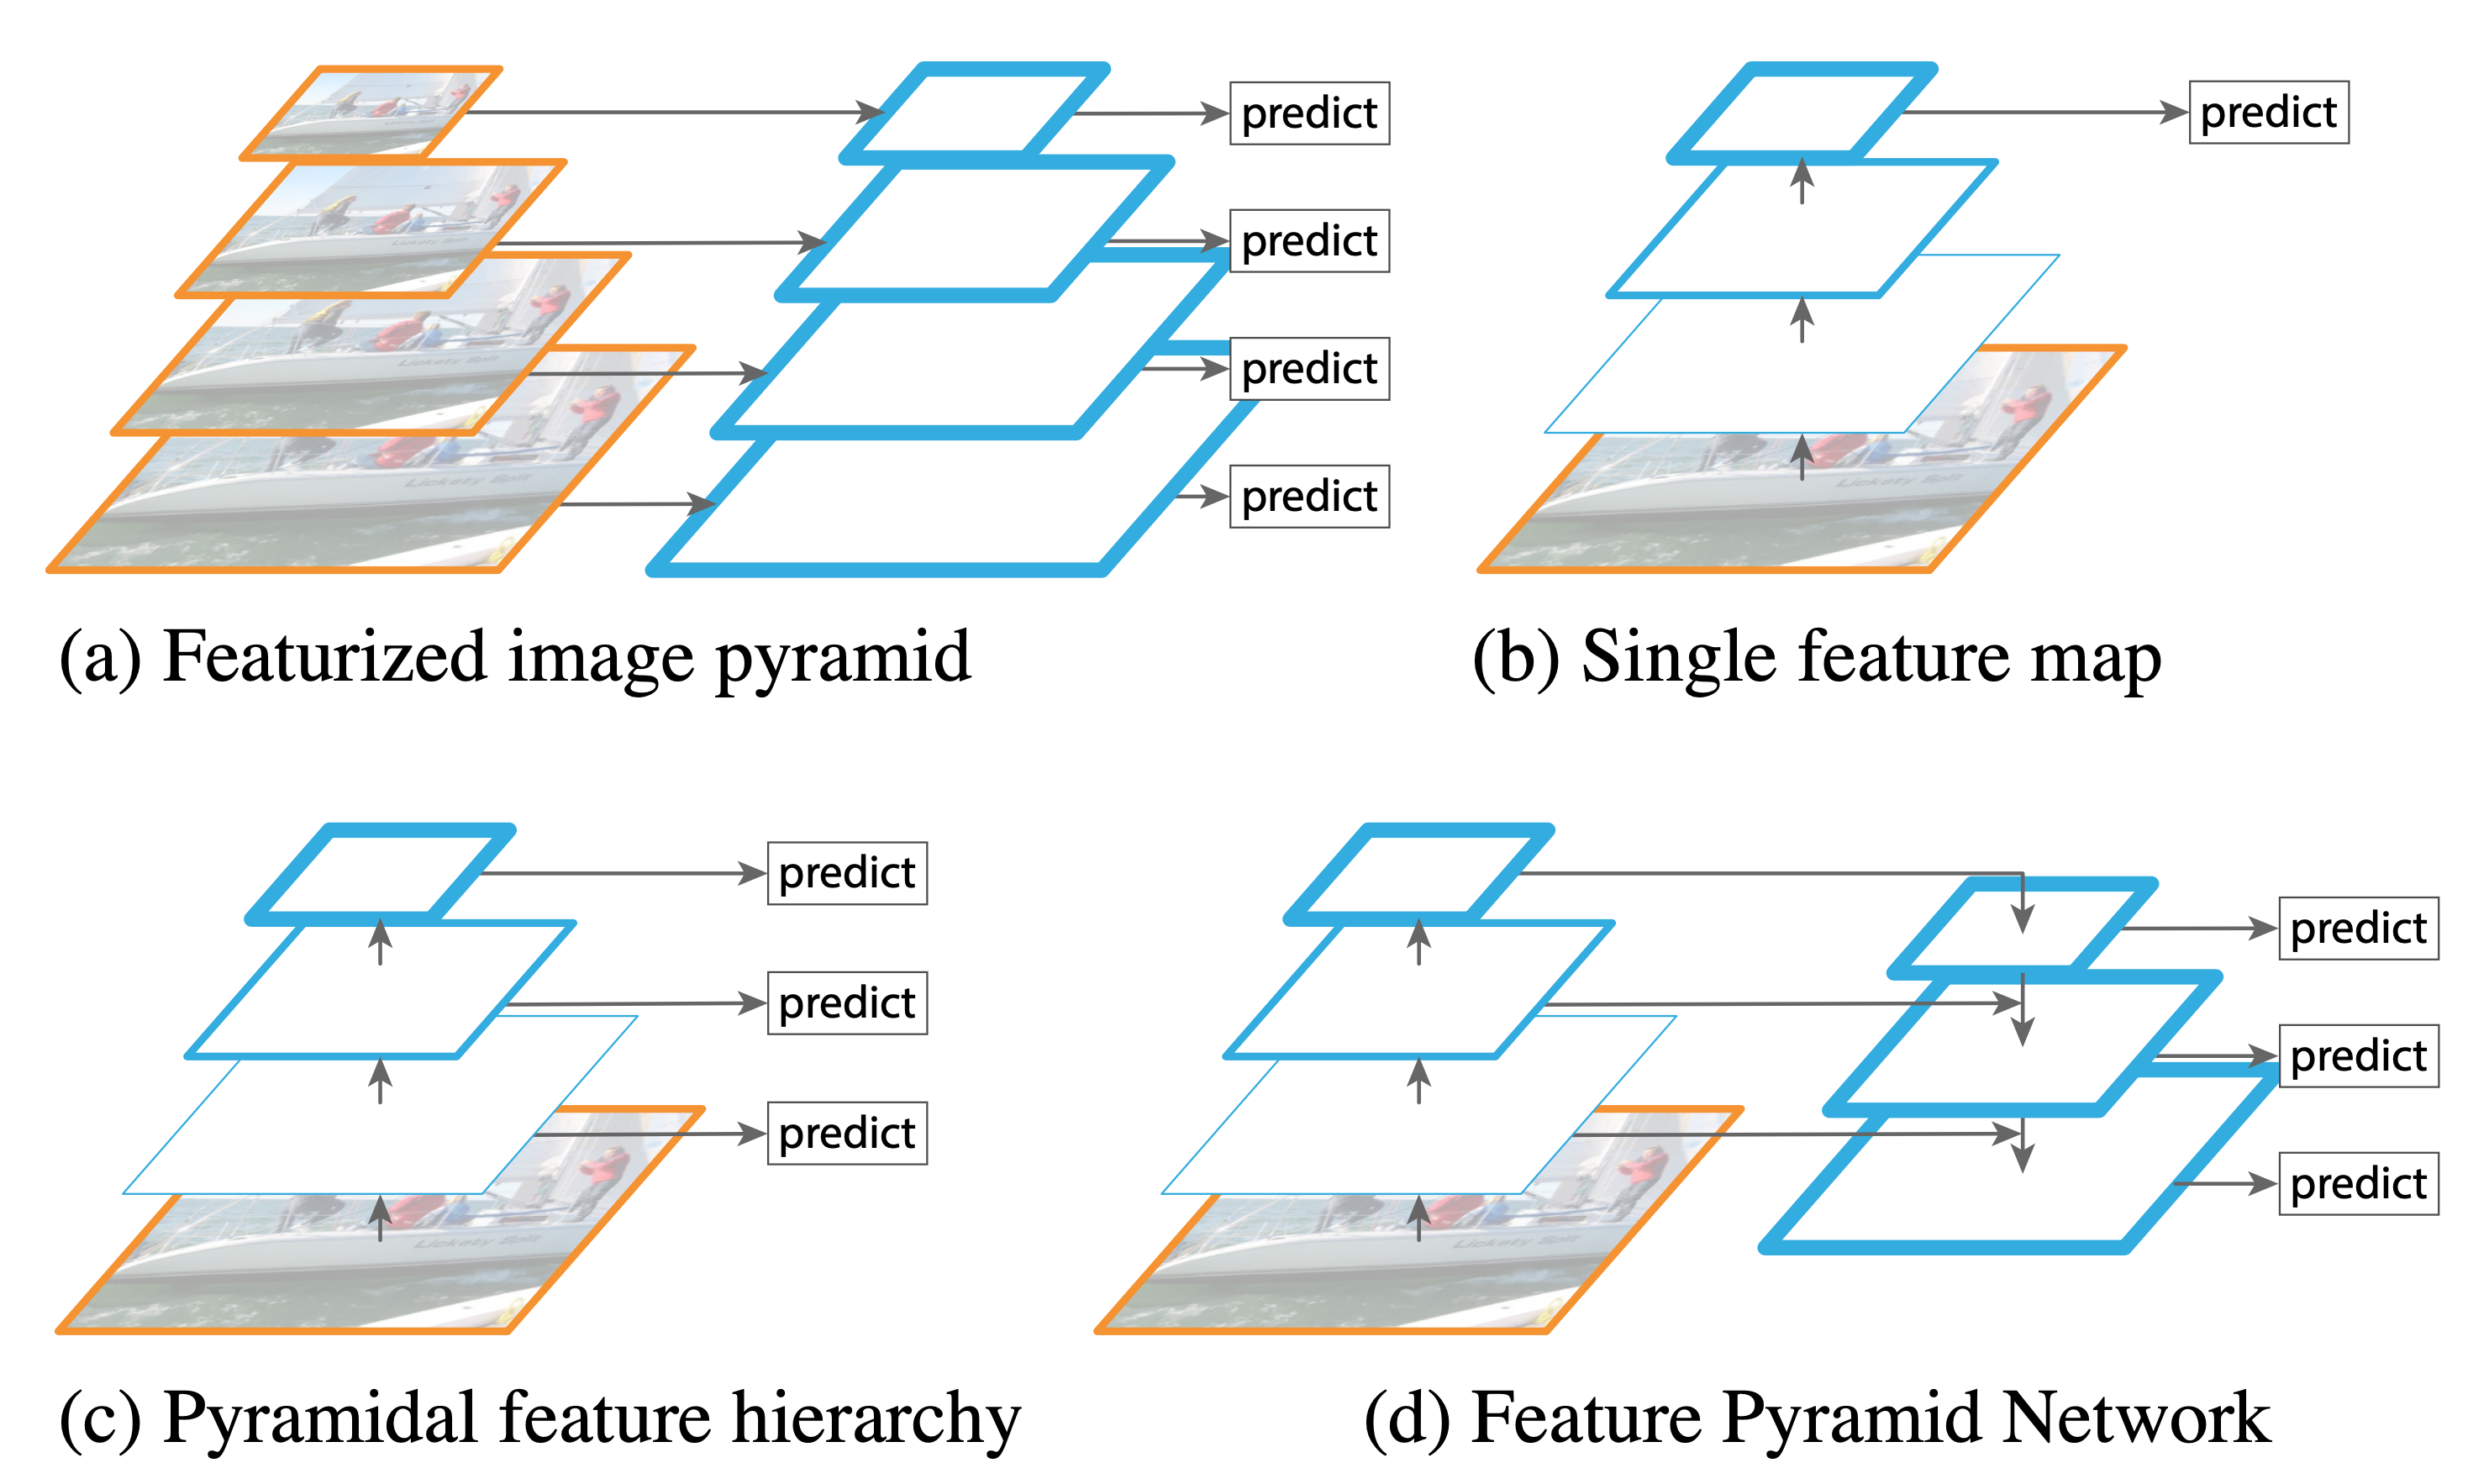
\includegraphics[width=11cm] {images/fpn_compare}
        \caption{So sánh các kiến trúc pyramid \index{kiến trúc pyramid} khác nhau (Nguồn: \cite{lin2017feature})}
        \label{fig:fpn_compare}
    \end{figure}

    \noindent
    Ý tưởng về việc xây dựng và sử dụng các đặc trưng của ảnh với nhiều kích thước khác nhau không mới, tuy nhiên, các giải pháp đã có vào thời điểm đó đều vướng phải một số vấn đề: \\
    - \textit{Featurized image pyramid} \index{Featurized image pyramid}: Việc sử dụng nhiều kích thước ảnh khác nhau để tạo ra nhiều đặc trưng có kích thước khác nhau một cách độc lập là ý tưởng cơ bản nhất. Mặc dù đạt được hiệu quả cao về độ chính xác khi khai thác ảnh đầu vào với nhiều kích thước khác nhau, nhưng phương pháp này khiến cho mô hình giải bài toán nhận diện đối tượng \index{nhận diện đối tượng} trở nên cồng kềnh và tốn rất nhiều thời gian để xử lý và gần như bất khả thi để có thể huấn luyện được mô hình. \\
    - \textit{Single feature map} \index{Single feature map}: Việc sử dụng chỉ một kích thước đặc trưng duy nhất giúp cho mô hình xử lý nhanh hơn nhưng lại khiến cho mô hình khó có thể học được những đặc trưng giữa các đối tượng có kích thước chênh lệch trong ảnh. Đặc biệt, việc đưa ảnh đầu vào qua nhiều khối Conv đã loại bỏ rất nhiều thông tin và gần như không còn thông tin để mô hình có thể nhận biết được các đối tượng có kích thước nhỏ. \\
    - \textit{Pyramidal feature hierarchy} \index{Pyramidal feature hierarchy}: Việc sử dụng nhiều feature maps \index{feature maps} có kích thước khác nhau cùng đưa ra kết quả được sử dụng trong mô hình nhận diện đối tượng \index{nhận diện đối tượng} khá nổi tiếng là SSD \index{SSD} \cite{liu2016ssd}. Tuy nhiên, thay vì tận dụng toàn bộ các feature maps \index{feature maps} sinh ra từ các khối Conv của backbone \index{backbone} VGG-16 \index{VGG-16}, SSD \index{SSD} chỉ sử dụng feature maps \index{feature maps} từ khối Conv thứ 5 và bổ sung thêm các lớp Conv \index{lớp Conv}. Điều này khiến cho SSD \index{SSD} bỏ qua những feature maps \index{feature maps} có kích thước lớn, có ý nghĩa quan trọng trong việc detect các đối tượng có kích thước nhỏ. \\
    - \textit{Feature Pyramid Network} \index{Feature Pyramid Network}: Dựa trên vấn đề trên từ SSD \index{SSD}, nhóm tác giả đề xuất FPN \index{FPN} tận dụng tối đa các feature maps \index{feature maps} trích xuất được từ backbone \index{backbone} nhằm tạo ra bộ feature maps \index{feature maps} mới gồm nhiều kích thước khác nhau và chứa rất nhiều thông tin về nội dung của ảnh đầu vào. Để đạt được điều này, nhóm tác giả thiết kế kiến trúc kết hợp những feature maps \index{feature maps} có kích thước lớn và những feature maps \index{feature maps} có kích thước nhỏ bằng top-down pathway \index{top-down pathway} và lateral connections \index{lateral connections}.

    \noindent
    \textbf{\textit{Kiến trúc mô hình Feature Pyramid Networks}} \\
    Ý tưởng về việc sử dụng kiến trúc mô hình theo dạng top-down không phải là mới và đã được nhắc đến trong một số nghiên cứu. Tuy nhiên, điểm giống nhau của các nghiên cứu có thiết kế mô hình theo kiểu top-down đó là mô hình chỉ sử dụng một feature maps \index{feature maps} cuối cùng, sau khi đã tổng hợp các thông tin trong suốt quá trình top-down, để đưa ra quyết định dự đoán cuối cùng.

    \noindent
    Trong khi đó, đối với FPN, nhóm tác giả đưa ra quyết định dự đoán trên từng feature maps \index{feature maps} trong suốt quá trình top-down. Từ đó, đặc biệt nâng cao chất lượng của mô hình nhận diện đối tượng \index{nhận diện đối tượng} khi có thể vừa trích xuất được thông tin của các đối tượng có kích thước lớn từ các feature maps \index{feature maps} có kích thước nhỏ vừa trích xuất được thông tin của các đối tượng có kích thước nhỏ từ các feature maps \index{feature maps} có kích thước lớn.

    \begin{figure}[H]
        \centering
        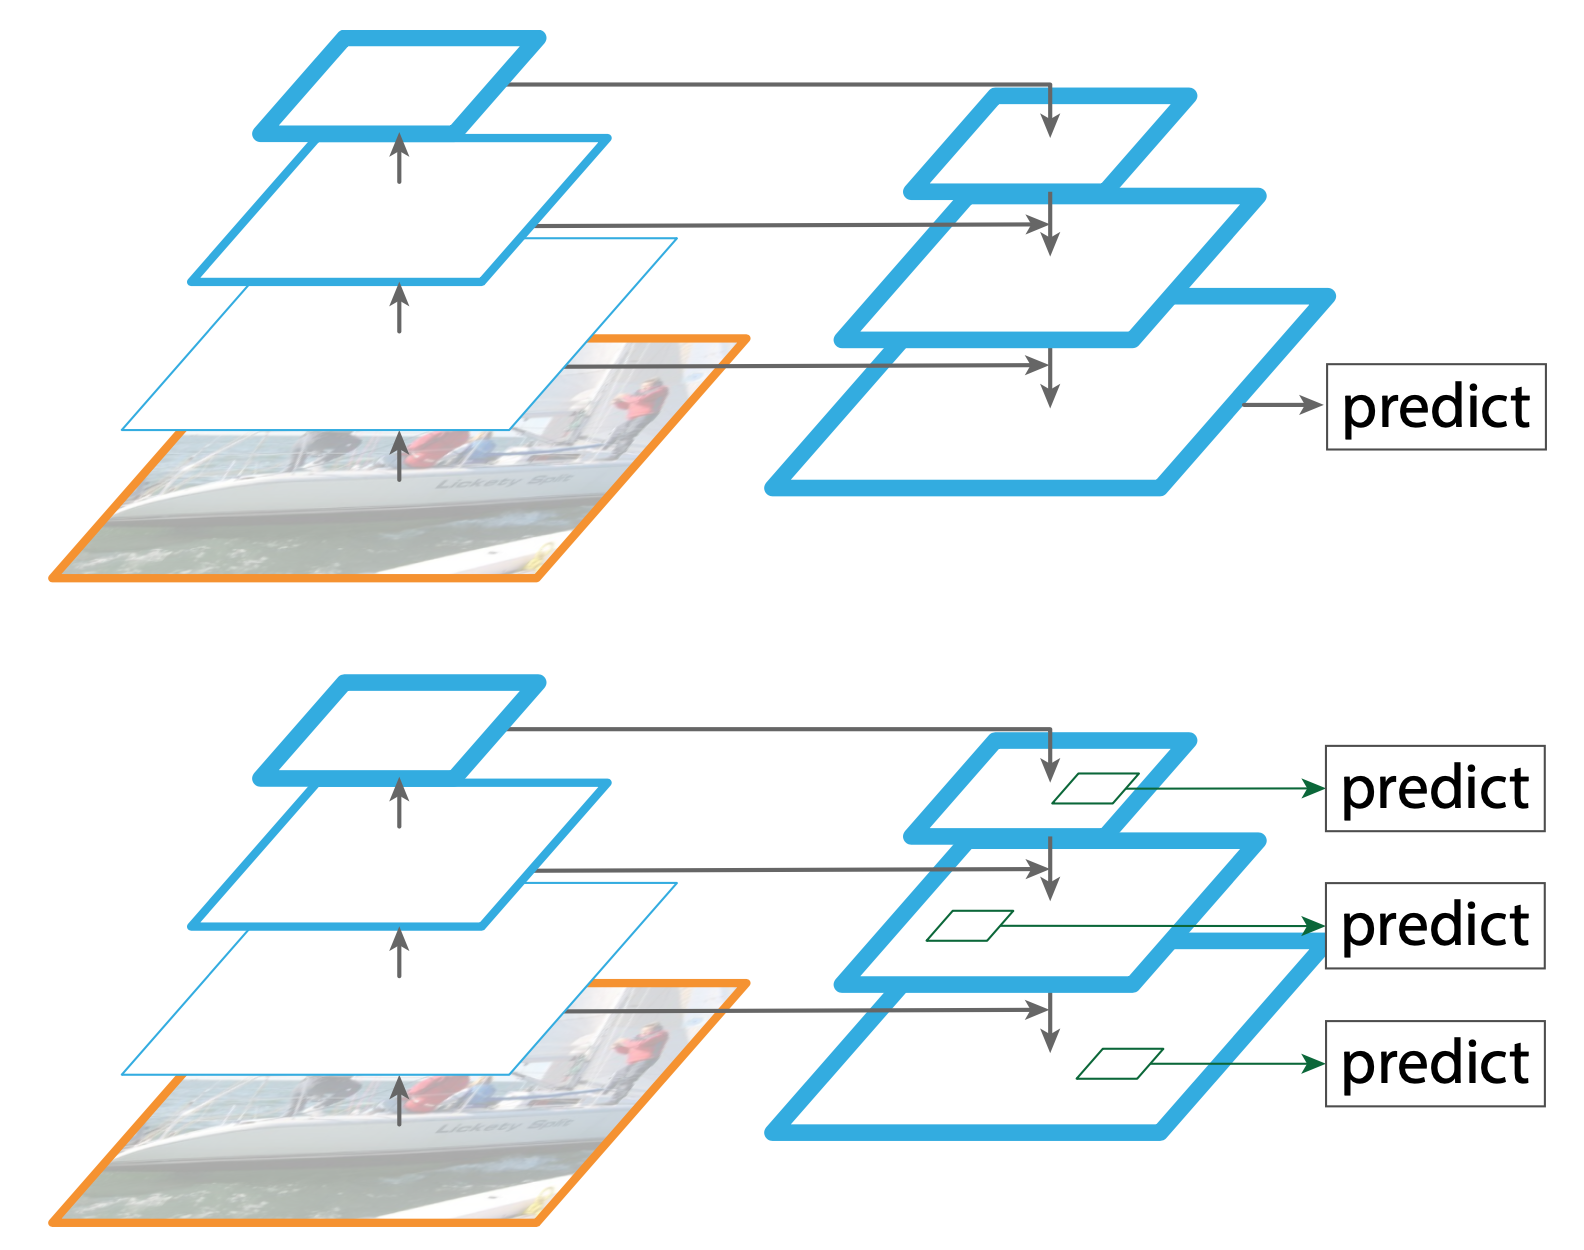
\includegraphics[width=6cm] {images/fpn_topdown}
        \caption{So sánh các kiến trúc theo dạng top-down khác nhau (Nguồn: \cite{lin2017feature})}
        \label{fig:fpn_topdown}
    \end{figure}

    \noindent
    Kiến trúc FPN \index{FPN} có thể được áp dụng với nhiều backbone \index{backbone} Conv khác nhau như AlexNet, VGG hay ResNet, cụ thể trong nghiên cứu, nhóm tác giả lựa chọn ResNet làm mô hình backbone.
    Kiến trúc FPN \index{FPN} có thể được chia làm hai phần: \\
    - \textit{Bottom-up pathway} \index{bottom-up pathway} là quá trình mà ta đưa ảnh đầu vào qua mô hình backbone \index{backbone} Conv như ResNet và thu được các feature maps \index{feature maps}.
    Tuy nhiên, trong các mô hình backbone \index{backbone} Conv, sẽ có một nhóm các lớp Conv \index{lớp Conv} tạo ra các feature maps \index{feature maps} có kích thước giống nhau, và nhóm các lớp Conv \index{lớp Conv} này được gọi là một khối Conv.
    Đối với FPN, nhóm tác giả lựa chọn các feature maps \index{feature maps} được sinh ra từ các lớp Conv \index{lớp Conv} cuối cùng trong mỗi khối Conv để sử dụng cho nhánh top-down pathway \index{top-down pathway}.
    Cụ thể đối với mô hình backbone \index{backbone} ResNet, nhóm tác giả sử dụng các feature maps \index{feature maps} được sinh ra từ residual block cuối cùng của mỗi khối Conv (trừ khối Conv đầu tiên do kích thước của feature maps \index{feature maps} này lớn và gây ra vấn đề về bộ nhớ), ký hiệu là \textit{{${C}_{2}, {C}_{3}, {C}_{4}, {C}_{5}$}}.
    Các feature maps \index{feature maps} này có kích thước lần lượt bằng 1/4, 1/8, 1/16 và 1/32 so với kích thước của ảnh đầu vào. \\
    - \textit{Top-down pathway và lateral connections} \index{top-down pathway} \index{lateral connections} là quá trình mà FPN \index{FPN} sinh ra thêm các feature maps \index{feature maps} mới từ các feature maps \index{feature maps} của bottom-up pathway \index{bottom-up pathway} và kết hợp chúng lại thông qua lateral connections \index{lateral connections}.
    Cụ thể, các feature maps \index{feature maps} của bottom-up pathway \index{bottom-up pathway} được đưa qua các lớp Conv \index{lớp Conv} có kích thước 1x1, stride \index{stride} bằng 1 nhằm giữ nguyên kích thước chiều dài, chiều rộng và chỉ thay đổi kích thước chiều channel \index{channel} của feature maps \index{feature maps}.
    Các feature maps \index{feature maps} ở vị trí cao hơn (có kích thước nhỏ hơn) được upsample \index{upsample} thông qua thuật toán nearest neighbor \index{nearest neighbor} và cộng ma trận với feature maps \index{feature maps} đầu ra từ lớp Conv \index{lớp Conv} 1x1 nói trên.
    Cuối cùng, các feature maps \index{feature maps} đầu ra từ phép cộng ma trận nói trên được đi qua một lớp Conv \index{lớp Conv} 3x3 có cùng số đầu ra channel \index{channel} của feature maps \index{feature maps} nhằm giảm bớt hiệu ứng của thuật toán nearest neighbor \index{nearest neighbor} và tạo ra các feature maps \index{feature maps} đầu ra cuối cùng có cùng số channel \index{channel} với nhau.
    Tập hợp feature maps \index{feature maps} này được gọi là \textit{{${P}_{2}, {P}_{3}, {P}_{4}, {P}_{5}$}} tương ứng với các feature maps \index{feature maps} có cùng kích thước \textit{{${C}_{2}, {C}_{3}, {C}_{4}, {C}_{5}$}}.

    \begin{figure}[H]
        \centering
        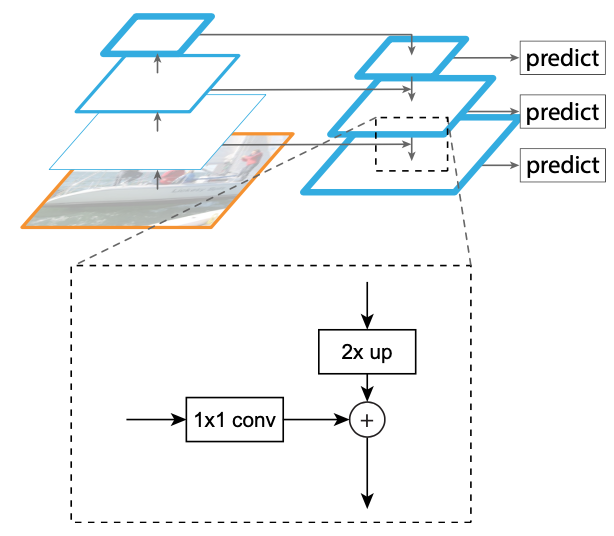
\includegraphics[width=6cm] {images/fpn_detail}
        \caption{Chi tiết kiến trúc FPN (Nguồn: \cite{lin2017feature})}
        \label{fig:fpn_detail}
    \end{figure}

    % \noindent
    % \textbf{\textit{Sử dụng kiến trúc FPN cho mô hình RPN}} \\
    % Ý tưởng về việc sử dụng kiến trúc FPN \index{FPN} cho mô hình RPN \index{RPN} \cite{ren2015faster} được nhóm tác giả đề xuất nhằm cải thiện khả năng đề xuất ra các khu vực có kích thước chênh lệch nhau.
    % Cụ thể, thay vì việc sử dụng một feature maps \index{feature maps} thu được từ feature extraction module \index{feature extraction module}, nhóm tác giả sử dụng các feature maps \index{feature maps} \textit{{${P}_{2}, {P}_{3}, {P}_{4}, {P}_{5}, {P}_{6}$}} (nhóm tác giả sử dụng thêm feature maps \index{feature maps} ${P}_{6}$ nhằm đề xuất ra những khu vực có kích thước lớn hơn).
    % Các feature maps \index{feature maps} này cùng được đưa qua một bộ các lớp Conv \index{lớp Conv} 3x3 và 1x1 chung để trả đầu ra kết quả anchor \index{anchor} có chứa đối tượng hay không và toạ độ của khu vực mà mô hình đề xuất.
    % Với việc sử dụng nhiều feature maps \index{feature maps} có các kích thước khác nhau, trên mỗi feature maps \index{feature maps}, nhóm tác giả chỉ sử dụng một kích thước anchor \index{anchor} lần lượt tương ứng \textit{{${32}^{2}, {64}^{2}, {128}^{2}, {256}^{2}, {512}^{2},$}} với ba tỷ lệ chiều dài giữa chiều rộng là \textit{1:2, 1:1, 2:1}.
    % Để có thể huấn luyện được, nhóm tác giả cũng sử dụng cơ chế gán positive/negative anchor \index{anchor} tương tự như chiến lược được đề xuất trong \cite{ren2015faster}.

    % \begin{figure}[H]
    %     \centering
    %     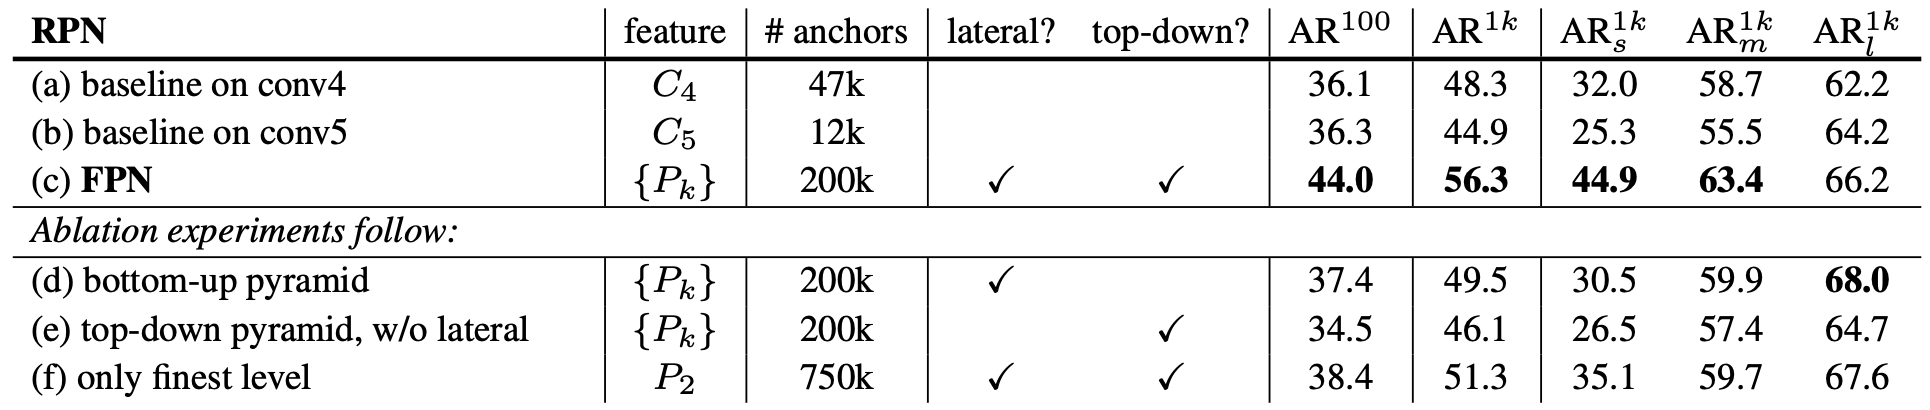
\includegraphics[width=12cm] {images/fpn_results_1}
    %     \caption{Kết quả của thí nghiệm sử dụng kiến trúc FPN cho mô hình RPN \index{RPN} \cite{ren2015faster} (Nguồn: \cite{lin2017feature})}
    %     \label{fig:fpn_results}
    % \end{figure}

    % \noindent
    % Kết quả của thí nghiệm sử dụng kiến trúc FPN \index{FPN} cho mô hình RPN \index{RPN} \cite{ren2015faster} được nhóm tác giả chia sẻ khá khả quan.
    % Ngoài việc so sánh việc sử dụng kiến trúc FPN \index{FPN} với các kiến trúc trước đây của mô hình RPN, nhóm tác giả còn so sánh thêm một số cấu hình khác của kiến trúc FPN \index{FPN}.
    % Cụ thể các cấu hình như sau: \\
    % - \textit{baseline on conv4} là cấu hình sử dụng feature maps \index{feature maps} từ lớp Conv \index{lớp Conv} thứ 4 của feature extraction module \index{feature extraction module} cho mô hình RPN. \\
    % - \textit{baseline on conv5} là cấu hình sử dụng feature maps \index{feature maps} từ lớp Conv \index{lớp Conv} thứ 5 của feature extraction module \index{feature extraction module} cho mô hình RPN. \\
    % - \textit{FPN} là cấu hình sử dụng kiến trúc FPN trích xuất các feature maps \index{feature maps} cho mô hình RPN. \\
    % - \textit{bottom-up pyramid} là cấu hình sử dụng các feature maps \index{feature maps} \textit{{${P}_{2}, {P}_{3}, {P}_{4}, {P}_{5}, {P}_{6}$}} cho mô hình RPN.
    % Tuy nhiên, giữa các feature maps \index{feature maps} này không có top-down pathway với nhau (hay nói cách khác, các feature maps \index{feature maps} \textit{{${P}_{2}, {P}_{3}, {P}_{4}, {P}_{5}, {P}_{6}$}} được sinh một cách độc lập từ các feature maps \index{feature maps} \textit{{${C}_{2}, {C}_{3}, {C}_{4}, {C}_{5}, {C}_{6}$}}). \\
    % - \textit{top-down pyramid, w/o lateral} là cấu hình sử dụng các feature maps \index{feature maps} \textit{{${P}_{2}, {P}_{3}, {P}_{4}, {P}_{5}, {P}_{6}$}} cho mô hình RPN.
    % Tuy nhiên, giữa các feature maps \index{feature maps} \textit{{${P}_{3}, {P}_{4}, {P}_{5}, {P}_{6}$}} không có lateral connections \index{lateral connections} với các feature maps \index{feature maps} \textit{{${C}_{3}, {C}_{4}, {C}_{5}, {C}_{6}$}} (hay nói cách khác, các feature maps \index{feature maps} \textit{{${P}_{3}, {P}_{4}, {P}_{5}, {P}_{6}$}} chỉ được sinh từ các feature maps \index{feature maps} \textit{{${P}_{2}, {P}_{3}, {P}_{4}, {P}_{5}$}}). \\
    % - \textit{only finest level} là cấu hình chỉ sử dụng duy nhất feature maps \index{feature maps} \textit{${P}_{2}$} cho mô hình RPN. \\
    % Trong đó, tất cả các cấu hình được huấn luyện với bộ dữ liệu \textit{COCO trainval135k} và kết quả thu được đánh giá trên bộ dữ liệu \textit{COCO minival}.
    % feature maps \index{feature maps} sử dụng trong cấu hình được ghi chú tại cột \textbf{feature}, số lượng khu vực được đề xuất trong quá trình test được thống kê tại cột \textbf{\# anchors}, cấu hình có sử dụng lateral connections \index{lateral connections} và top-down pathway hay không được chú thích tại cột \textbf{lateral} và \textbf{top-down}. \\
    % Cấu hình \textit{FPN} đạt kết quả cao hơn vượt trội so với các cấu hình \textit{baseline on conv4} và \textit{baseline on conv5} nguyên bản.
    % Cấu hình \textit{FPN} chỉ đạt kết quả kém hơn so với cấu hình \textit{bottom-up pyramid} khi so sánh trên chỉ số đánh giá với những bounding box \index{bounding box} có kích thước lớn, tuy nhiên, sự chênh lệch giữa hai cấu hình là không quá khác biệt.

    % \noindent
    % \textbf{\textit{Sử dụng kiến trúc FPN cho mô hình Fast R-CNN \index{Fast R-CNN}}} \\
    % Ý tưởng về việc sử dụng kiến trúc FPN cho mô hình Fast R-CNN \index{Fast R-CNN} được nhóm tác giả đề xuất nhằm cải thiện khả năng định vị ra bounding box \index{bounding box} từ các khu vực đã được đề xuất từ mô hình RPN.
    % Cụ thể, sau khi đưa ảnh qua region proposals module \index{region proposals module} của mô hình Fast R-CNN \index{Fast R-CNN} là Selective Search, ta thu được toạ độ của khu vực được đề xuất trên ảnh đầu vào.
    % Đối với mô hình Fast R-CNN \index{Fast R-CNN} nguyên bản, ta dễ dàng lấy được khu vực đề xuất trên feature maps \index{feature maps} của ảnh đầu vào, tuy nhiên, với việc sử dụng kiến trúc FPN cho feature extraction module \index{feature extraction module}, câu hỏi đặt ra là đối với từng khu vực đề xuất ta xác định feature maps \index{feature maps} nào trong số \textit{{${P}_{2}, {P}_{3}, {P}_{4}, {P}_{5}$}} để lấy làm đầu vào cho lớp RoI pooling?
    % Nhóm tác giả đã coi danh sách feature maps \index{feature maps} \textit{{${P}_{2}, {P}_{3}, {P}_{4}, {P}_{5}$}} sinh ra bởi FPN tương tự với các feature maps \index{feature maps} được sinh ra từ việc sử dụng image pyramids và áp dụng công thức sau để xác định feature maps \index{feature maps} phù hợp cho từng khu vực làm đầu vào của lớp RoI pooling.

    % \begin{equation}
    %     \label{eq:roi_mapping}
    %     k = \lfloor k_0 + \log_2(\sqrt{wh} / 224) \rfloor.
    % \end{equation}

    % \noindent
    % trong đó: \\
    % \textit{k} là index của feature maps \index{feature maps} sử dụng làm đầu vào cho lớp RoI pooling tương ứng với khu vực đề xuất có kích thước chiều rộng là \textit{w} và chiều cao là \textit{h} \\
    % $k_0$ là index của feature maps \index{feature maps} sử dụng làm đầu vào cho lớp RoI pooling tương ứng với khu vực đề xuất có kích thước chiều rộng và chiều cao lần lượt là 224 và 224 \\
    % Tác giả lựa chọn con số 224 bởi đây là kích thước ảnh của pretrained ImageNet và lựa chọn $k_0 = 4$. \\
    % Các feature maps \index{feature maps} được lấy ra tương ứng với từng khu vực đề xuất được đưa qua lớp lớp RoI pooling có kích thước đầu ra là 7x7 và được đưa qua chung các lớp Conv \index{lớp Conv} và lớp fully connected \index{lớp fully connected} để xác định lớp của đối tượng và toạ độ của bounding box \index{bounding box}.

    % \begin{figure}[H]
    %     \centering
    %     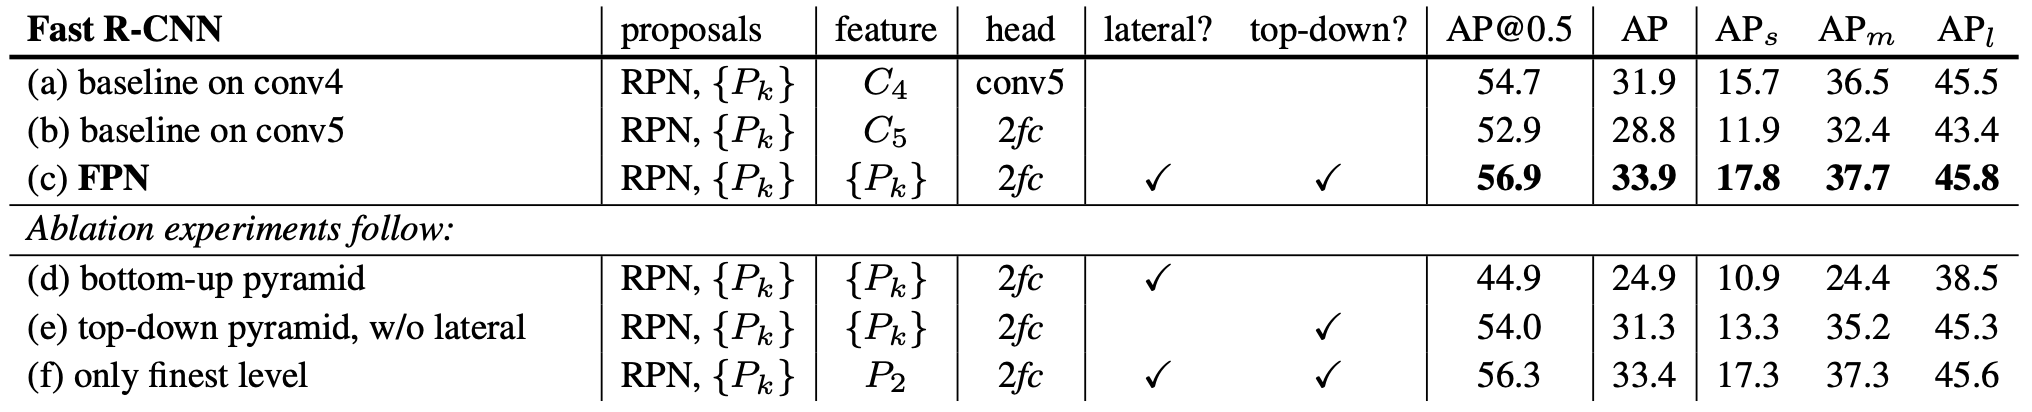
\includegraphics[width=12cm] {images/fpn_results_2}
    %     \caption{Kết quả của thí nghiệm sử dụng kiến trúc FPN cho mô hình Fast R-CNN \index{Fast R-CNN} (Nguồn: \cite{lin2017feature})}
    %     \label{fig:fpn_results}
    % \end{figure}
    
    % \noindent
    % Kết quả của thí nghiệm sử dụng kiến trúc FPN cho mô hình Fast R-CNN \index{Fast R-CNN} được nhóm tác giả chia sẻ khá ấn tượng.
    % Ngoài việc so sánh việc sử dụng kiến trúc FPN với các kiến trúc trước đây của mô hình Fast R-CNN \index{Fast R-CNN}, nhóm tác giả còn so sánh thêm một số cấu hình khác của kiến trúc FPN.
    % Cụ thể các cấu hình như sau: \\
    % - \textit{baseline on conv4} là cấu hình sử dụng feature maps \index{feature maps} từ lớp Conv \index{lớp Conv} thứ 4 của feature extraction module \index{feature extraction module} cho mô hình Fast R-CNN \index{Fast R-CNN}. \\
    % - \textit{baseline on conv5} là cấu hình sử dụng feature maps \index{feature maps} từ lớp Conv \index{lớp Conv} thứ 5 của feature extraction module \index{feature extraction module} cho mô hình Fast R-CNN \index{Fast R-CNN}. \\
    % - \textit{FPN} là cấu hình sử dụng kiến trúc FPN trích xuất feature maps \index{feature maps} cho mô hình Fast R-CNN \index{Fast R-CNN} như mô tả ở trên. \\
    % - \textit{bottom-up pyramid} là cấu hình sử dụng các feature maps \index{feature maps} \textit{{${P}_{2}, {P}_{3}, {P}_{4}, {P}_{5}, {P}_{6}$}} cho mô hình Fast R-CNN \index{Fast R-CNN}.
    % Tuy nhiên, giữa các feature maps \index{feature maps} này không có top-down pathway với nhau (hay nói cách khác, các feature maps \index{feature maps} \textit{{${P}_{2}, {P}_{3}, {P}_{4}, {P}_{5}, {P}_{6}$}} được sinh một cách độc lập từ các feature maps \index{feature maps} \textit{{${C}_{2}, {C}_{3}, {C}_{4}, {C}_{5}, {C}_{6}$}}). \\
    % - \textit{top-down pyramid, w/o lateral} là cấu hình sử dụng các feature maps \index{feature maps} \textit{{${P}_{2}, {P}_{3}, {P}_{4}, {P}_{5}, {P}_{6}$}} cho mô hình Fast R-CNN \index{Fast R-CNN}.
    % - \textit{only finest level} là cấu hình chỉ sử dụng duy nhất feature maps \index{feature maps} \textit{${P}_{2}$} cho mô hình Fast R-CNN \index{Fast R-CNN}. \\
    % Trong đó, tất cả các cấu hình được huấn luyện với bộ dữ liệu \textit{COCO trainval135k} và kết quả thu được đánh giá trên bộ dữ liệu \textit{COCO minival} và cùng sử dụng chung một bộ khu vực đề xuất từ mô hình RPN.
    % feature maps \index{feature maps} sử dụng trong cấu hình được ghi chú tại cột \textbf{feature}, kiến trúc mô hình RPN \index{RPN} \cite{ren2015faster} sử dụng trong từng cấu hình được chú thích tại cột \textbf{proposals}, cấu hình của phần head của mô hình Fast R-CNN \index{Fast R-CNN} được chú thích tại cột \textbf{head}, cấu hình có sử dụng lateral connections \index{lateral connections} và top-down pathway hay không được chú thích tại cột \textbf{lateral} và \textbf{top-down}. \\
    % Cấu hình \textit{FPN} đạt kết quả cao hơn vượt trội so với các cấu hình \textit{baseline on conv4}, \textit{baseline on conv5} nguyên bản và cả các cấu hình tuỳ chọn như \textit{bottom-up pyramid}, \textit{top-down pyramid, w/o lateral}, \textit{only finest level}.

    % \noindent
    % \textbf{\textit{Sử dụng kiến trúc FPN cho toàn bộ các thành phần của mô hình Faster R-CNN}} \\
    % Nhóm tác giả còn thực hiện một thí nghiệm nữa với kiến trúc FPN khi sử dụng FPN chung cho toàn bộ cả mô hình RPN \index{RPN} \cite{ren2015faster} và mô hình Fast R-CNN \index{Fast R-CNN} (mô hình RPN \index{RPN} \cite{ren2015faster} và mô hình Fast R-CNN \index{Fast R-CNN} sử dụng chung một kiến trúc backbone \index{backbone} FPN) và cũng đạt kết quả tương đối tốt.

    % \begin{figure}[H]
    %     \centering
    %     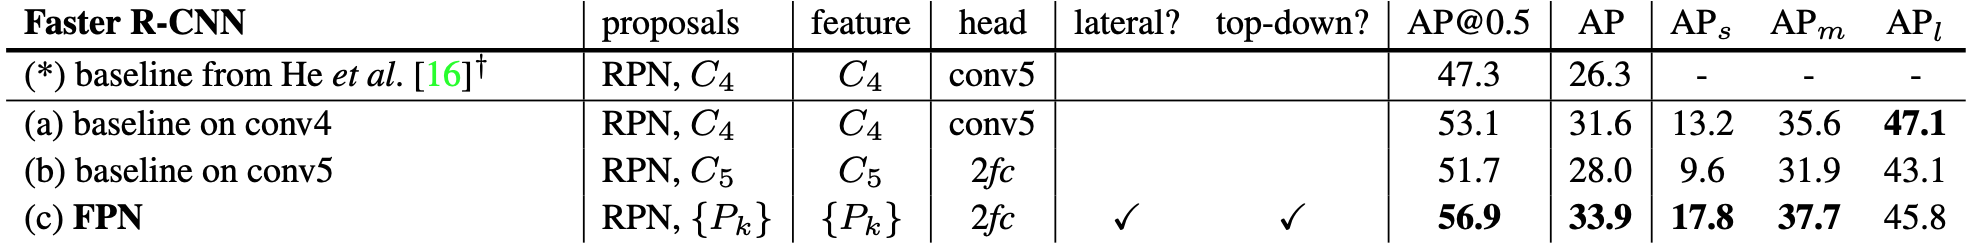
\includegraphics[width=12cm] {images/fpn_results_3}
    %     \caption{Kết quả của thí nghiệm sử dụng kiến trúc FPN cho mô hình Faster R-CNN \index{Faster R-CNN} (Nguồn: \cite{lin2017feature})}
    %     \label{fig:fpn_results_3}
    % \end{figure}

    % \noindent
    % Cụ thể các cấu hình như sau: \\
    % - \textit{baseline from He et al.} là mô hình ResNet được sử dụng cho bài toán nhận diện đối tượng \index{nhận diện đối tượng}. \\
    % - \textit{baseline on conv4} là cấu hình sử dụng feature maps \index{feature maps} từ lớp Conv \index{lớp Conv} thứ 4 của feature extraction module \index{feature extraction module} cho cả hai nhánh của mô hình Faster R-CNN \index{Faster R-CNN}. \\
    % - \textit{baseline on conv5} là cấu hình sử dụng feature maps \index{feature maps} từ lớp Conv \index{lớp Conv} thứ 5 của feature extraction module \index{feature extraction module} cho cả hai nhánh của mô hình Faster R-CNN \index{Faster R-CNN}. \\
    % - \textit{FPN} là cấu hình sử dụng kiến trúc FPN trích xuất feature maps \index{feature maps} cho cả hai nhánh của mô hình Faster R-CNN \index{Faster R-CNN}. \\
    % Trong đó, tất cả các cấu hình được huấn luyện với bộ dữ liệu \textit{COCO trainval135k} và kết quả thu được đánh giá trên bộ dữ liệu \textit{COCO minival}.
    % feature maps \index{feature maps} sử dụng trong cấu hình được ghi chú tại cột \textbf{feature}, kiến trúc mô hình RPN \index{RPN} \cite{ren2015faster} sử dụng trong từng cấu hình được chú thích tại cột \textbf{proposals}, cấu hình của phần head của mô hình Fast R-CNN \index{Fast R-CNN} được chú thích tại cột \textbf{head}, cấu hình có sử dụng lateral connections \index{lateral connections} và top-down pathway hay không được chú thích tại cột \textbf{lateral} và \textbf{top-down}. \\
    % Cấu hình \textit{FPN} đạt kết quả cao hơn vượt trội so với các cấu hình còn lại trên hầu hết các chỉ số đánh giá.
    % Chỉ có duy nhất chỉ số trên đối với các bounding box \index{bounding box} có kích thước lớn thì kết quả của cấu hình \textit{FPN} kém hơn một chút so với cấu hình \textit{baseline on conv4}.

    \noindent
    \textbf{\textit{Vấn đề tồn đọng của kiến trúc mô hình FPN}} \\
    Kiến trúc FPN ra đời đã tạo ra một trong số những kiến trúc backbone \index{backbone} kinh điển trong bài toán nhận diện đối tượng \index{nhận diện đối tượng} nói riêng.
    Kiến trúc FPN đã giúp cho nhiều mô hình đạt độ chính xác cao hơn và trong khi tốc độ của mô hình không bị tăng một cách đáng kể.
    Tuy nhiên, đối với cụ thể bài toán nhận diện đối tượng \index{nhận diện đối tượng}, việc kết hợp kiến trúc FPN vào mô hình Faster R-CNN \index{Faster R-CNN} mới chỉ cải thiện về mặt độ chính xác cho mô hình Faster R-CNN \index{Faster R-CNN} mà chưa giúp tăng tốc mô hình Faster R-CNN \index{Faster R-CNN}.
    Vẫn còn một câu hỏi cần phải được giải quyết đó là làm sao để duy trì được độ chính xác mà FPN mang lại những mô hình nhận diện đối tượng \index{nhận diện đối tượng} vẫn có để đạt tốc độ nhanh hơn nữa.
}
    \fpn

    \subsection{Mô hình RetinaNet}
    \def\retinanet{
    RetinaNet \cite{lin2017focal} là một mô hình single-stage object detection cân bằng giữa độ chính xác của các mô hình two-stage và tốc độ của các mô hình single-stage ở thời điểm đó.
    Nhóm tác giả của RetinaNet đưa ra vấn đề về các mô hình single-stage như YOLO \cite{redmon2016look} hay SSD \cite{liu2016ssd} dù đạt tốc độ rất nhanh nhưng lại kém các mô hình two-stage một khoảng rất xa về độ chính xác và đề xuất giải pháp khắc phục vấn đề này.

    \noindent
    \textbf{\textit{Tổng quan về các mô hình single-stage object detection}} \\
    Các mô hình single-stage object detection ở thời điểm đó đa phần đều chỉ sử dụng một backbone CNN kết hợp thêm với các lớp Conv và lớp fully connected để đưa ra dự đoán về lớp của đối tượng trong ảnh và độ lệch của bounding box so với groundtruth.
    
    \begin{figure}[H]
        \centering
        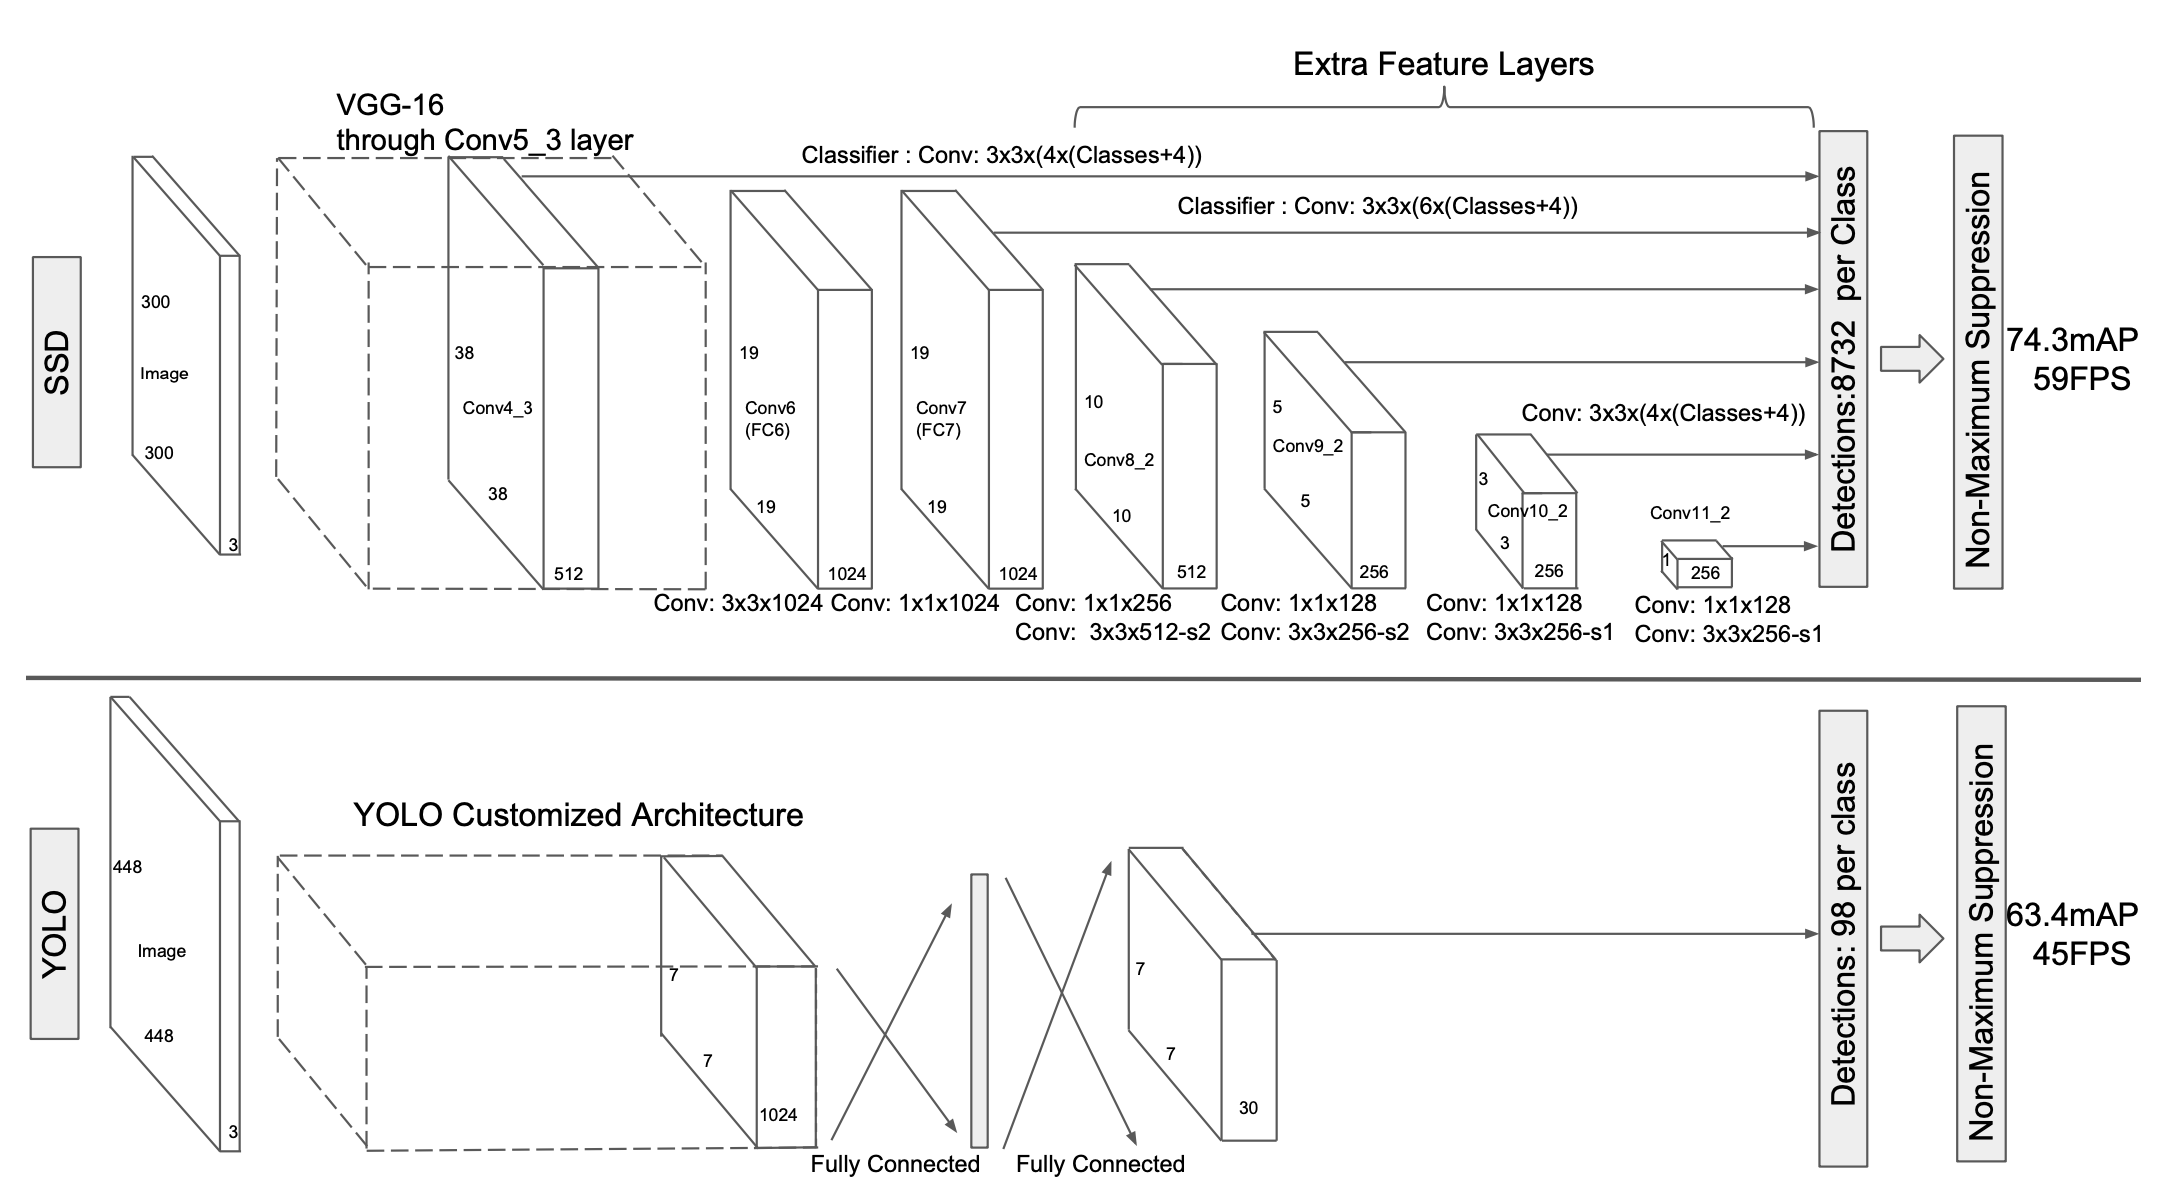
\includegraphics[width=10cm] {images/yolo_ssd_model}
        \caption{Chi tiết hai kiến trúc mô hình single-stage nổi tiếng là SSD và YOLO. (Nguồn: \cite{liu2016ssd})}
        \label{fig:yolo_ssd_model}
    \end{figure}

    \noindent
    Việc loại bỏ Region proposals module khiến các mô hình single-stage object detection cần phải xây dựng một phương pháp riêng nhằm đề xuất ra các anchor chứa đối tượng.
    Hai mô hình single-stage object detection nổi tiếng vào thời điểm đó là YOLO \cite{redmon2016look} và SSD \cite{liu2016ssd} có các cách đề xuất ra anchor tương tự với nhau.
    
    \begin{figure}[H]
        \centering
        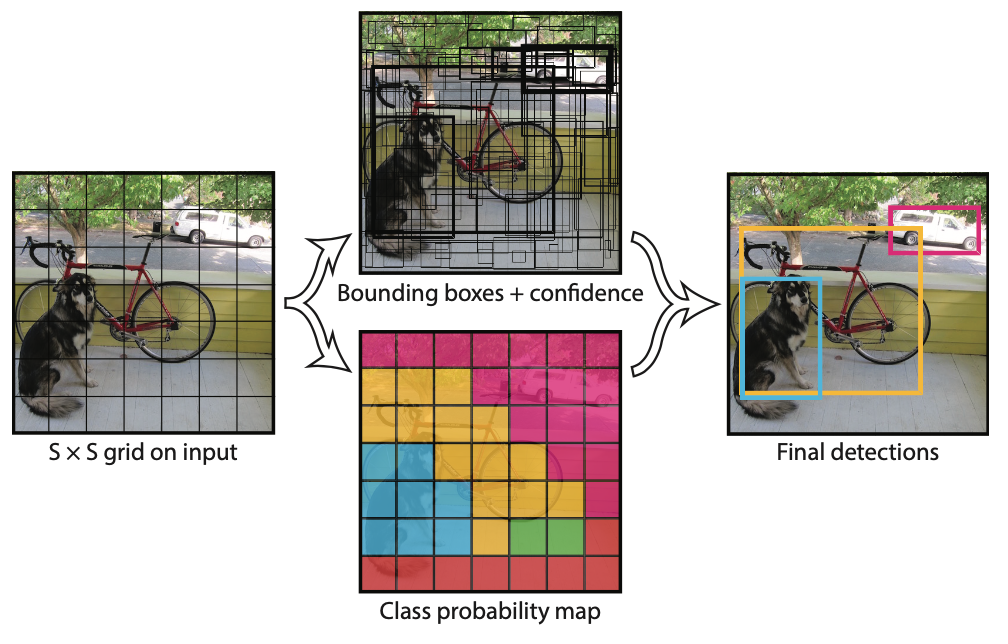
\includegraphics[width=10cm] {images/yolo_anchor}
        \caption{Cách đề xuất anchor của mô hình YOLO. (Nguồn: \cite{redmon2016look})}
        \label{fig:yolo_anchor}
    \end{figure}

    \noindent
    YOLO đề xuất ra các anchor thông qua việc chia ảnh đầu vào thành dạng grid có kích thước $S × S$ và với mỗi grid sẽ trả đầu ra dự đoán có kích thước $S × S × (B * 5 + C)$.
    Nếu tâm của một bounding box nằm trong ô nào trên grid, ô đó sẽ cần phải được dự đoán là chứa đối tượng.
    Mỗi ô trên grid sẽ được mô hình dự đoán $(B * 5 + C)$ giá trị, trong đó: \\
    - B là số lượng bounding box dự đoán. \\
    - 5 là các giá trị trong đó có 4 giá trị x, y, w, h đại diện cho bounding box được dự đoán và 1 giá trị confidence.
    Thay vì được học là 1 nếu anchor có IoU cao với groundtruth bounding box và ngược lại là 0 nếu anchor có IoU thấp với groundtruth bounding box, điểm đặc biệt về giá trị confidence mà nhóm tác giả thiết kế trong mô hình YOLO là nó bằng chính giá trị IoU so với groundtruth. \\
    - C là số lượng lớp đối tượng trong bài toán object detection.
    Mỗi giá trị dự đoán trong C là giá trị xác suất điều kiện nếu ô trên grid chứa đối tượng thì đó là đối tượng nào. \\
    Trong nghiên cứu, nhóm tác giả của YOLO sử dụng $S = 7, B = 2, C = 20$.

    \begin{figure}[H]
        \centering
        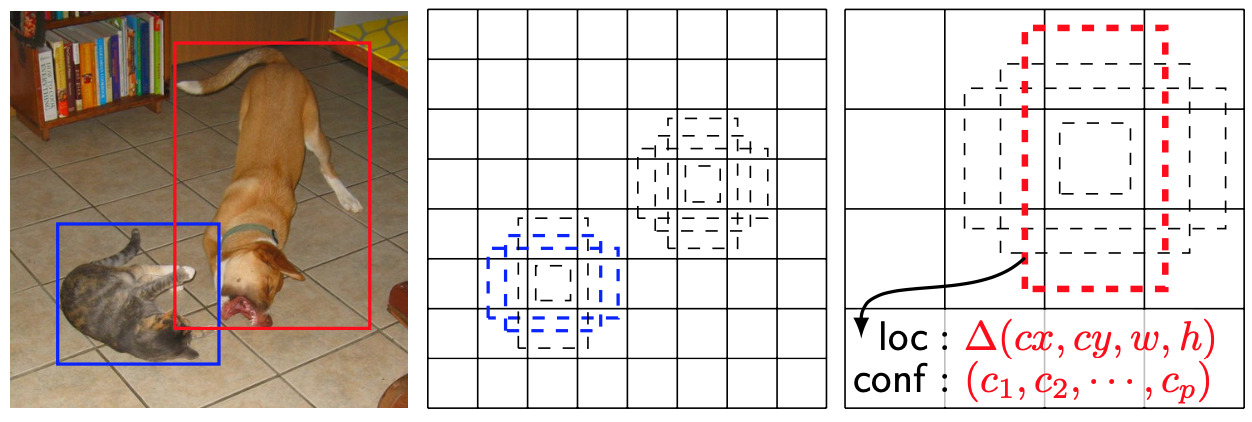
\includegraphics[width=10cm] {images/ssd_anchor}
        \caption{Cách đề xuất anchor của mô hình SSD. (Nguồn: \cite{liu2016ssd})}
        \label{fig:ssd_anchor}
    \end{figure}
    
    \noindent
    SSD cũng sử dụng feature maps như là các dạng grid của ảnh đầu vào nhưng thay vì sử dụng một grid như YOLO thì SSD sử dụng nhiều grid từ nhiều feature maps có cách kích thước khác nhau.
    Với mỗi grid tạo bởi một feature maps có kích thước $m × n$, SSD trả đầu ra dự đoán có kích thước $m × n × (k × (c + 4))$.
    Nếu tâm của một bounding box nằm trong ô nào trên grid, ô đó sẽ cần phải được dự đoán là chứa đối tượng.
    Mỗi ô trên grid sẽ được mô hình dự đoán $(k × (c + 4))$ giá trị, trong đó: \\
    - k là số lượng bounding box dự đoán. \\
    - 4 là 4 giá trị x, y, w, h đại diện cho bounding box được dự đoán. \\
    - c là số lượng lớp đối tượng trong bài toán object detection.
    Mỗi giá trị dự đoán trong c là giá trị xác suất anchor đó là đối tượng nào.

    \noindent
    Với ý tưởng khởi tạo anchor như trên, nhóm tác giả của RetinaNet đã chỉ ra một vấn đề nghiêm trọng mà các mô hình single stage object detection nói chung gặp phải đó là vấn đề mất cân bằng dữ liệu trong quá trình train mô hình.
    Cụ thể, vấn đề mất cân bằng ở đây xảy ra chủ yếu do sự chênh lệch giữa phần ảnh là foreground và phần ảnh là background, hay nói cách khác là phần ảnh chứa đối tượng và phần ảnh không chứa đối tượng. \\
    Các mô hình two-stage object detection không thật sự gặp phải vấn đề mất cân bằng dữ liệu này bởi vì trong quá trình đưa các khu vực đề xuất từ Region proposals module sang Feature extraction module thường đã có một bước lọc và lựa chọn.
    Cụ thể hơn, với số lượng lớn các khu vực không chứa đối tượng được đề xuất bởi Region proposals module, chỉ có một số ít trong đó được lựa chọn để làm đầu vào cho Feature extraction module và lúc này, tỷ lệ giữa các khu vực chứa và không chứa đối tượng thường là 1:3 - một tỷ lệ mất cân bằng không quá nghiêm trọng và không ảnh hưởng tới việc train mô hình object detection.

    \noindent
    \textbf{\textit{Hàm Focal loss}} \\
    Để giải quyết vấn đề mất cân bằng dữ liệu nói trên, nhóm tác giả của RetinaNet đã đề xuất hàm Focal loss dựa trên nền tảng của hàm binary cross entropy loss giải quyết vấn đề mất cân bằng dữ liệu nghiêm trọng.
    Nhóm tác giả chú thích rằng hàm Focal loss hiệu quả đối với cả bài toán phân lớp với nhiều hơn hai lớp nhưng để đơn giản hoá, nhóm tác giả sử dụng hàm binary cross entropy loss.

    \begin{equation}
        \label{eq:bce}
        CE(p,y) = 
        \begin{cases}
            -\log(p) &\text{if $y = 1$} \\
            -\log (1 - p) &\text{otherwise.}
        \end{cases}
    \end{equation}

    \noindent
    trong đó: \\
    - y là giá trị groundtruth (0 đối với anchor không chứa object và 1 đối với anchor chứa object) \\
    - p là giá trị xác suất mà mô hình dự đoán anchor đó chứa object \\
    Để ngắn gọn, nhóm tác giả quy ước lại như sau:

    \begin{equation}
        \label{eq:bce}
        p_\textrm{t} =
        \begin{cases}
            p &\text{if $y = 1$} \\
            1 - p &\text{otherwise,}
        \end{cases}
    \end{equation}

    \noindent
    từ đó, hàm cross entropy loss được viết lại thành

    \begin{equation}
        CE(p,y) = CE(p_\textrm{t}) = - \log (p_\textrm{t})
    \end{equation}

    \noindent
    Một cấu hình khác của hàm cross entropy loss là \textit{balanced cross entropy loss}, được sinh ra bằng việc đánh trọng số cho từng số hạng của hàm cross entropy loss ban đầu

    \begin{equation}
        CE(p,y) = - \alpha_\textrm{t} \log (p_\textrm{t})
    \end{equation}

    \noindent
    trong đó: \\
    - $\alpha_\textrm{t}$ là trọng số tương ứng với số hạng $p_\textrm{t}$.
    Trọng số $\alpha_\textrm{t}$ có thể được tính dựa trên tần suất xuất hiện của các lớp trong bộ dữ liệu hoặc là một hyperpameter.

    \noindent
    Hàm balanced cross entropy loss có thể đã giúp giảm bớt hiệu ứng mất cân bằng dữ liệu lên trên giá trị hàm loss.
    Tuy nhiên, việc gán trọng số như hàm balanced cross entropy loss không phân biệt được giữa những mẫu dữ liệu dễ và khó.
    Nhóm tác giả, từ đó, đề xuất hàm \textit{Focal loss} không những giúp giải quyết vấn đề mất cân bằng dữ liệu mà còn giúp mô hình tập trung vào những mẫu dữ liệu \textit{không chứa đối tượng} nhưng khó và dễ nhầm lẫn thành \textit{chứa đối tượng}.

    \begin{equation}
        FL(p_\textrm{t}) = - (1 - p_\textrm{t})^\gamma \log (p_\textrm{t})
    \end{equation}

    \noindent
    trong đó: \\
    - $(1 - p_\textrm{t})$ là thành phần đánh giá độ dễ hay khó của mẫu dữ liệu.
    Với những mẫu dễ và mô hình đã được train tốt, giá trị $(1 - p_\textrm{t})$ sẽ nhỏ và những mẫu này sẽ gây ít ảnh hưởng trong quá trình train mô hình. \\
    - $\gamma$ được nhóm tác giả gọi là \textit{focusing parameter}, dùng để xác định mức độ tập trung của mô hình lên các mẫu dữ liệu không chứa đối tượng.
    Với $\gamma = 0$, hàm FL lúc này tương tự với hàm CE.
    Trong các thí nghiệm của RetinaNet, giá trị $\gamma = 2$ là tốt nhất.

    \begin{figure}[H]
        \centering
        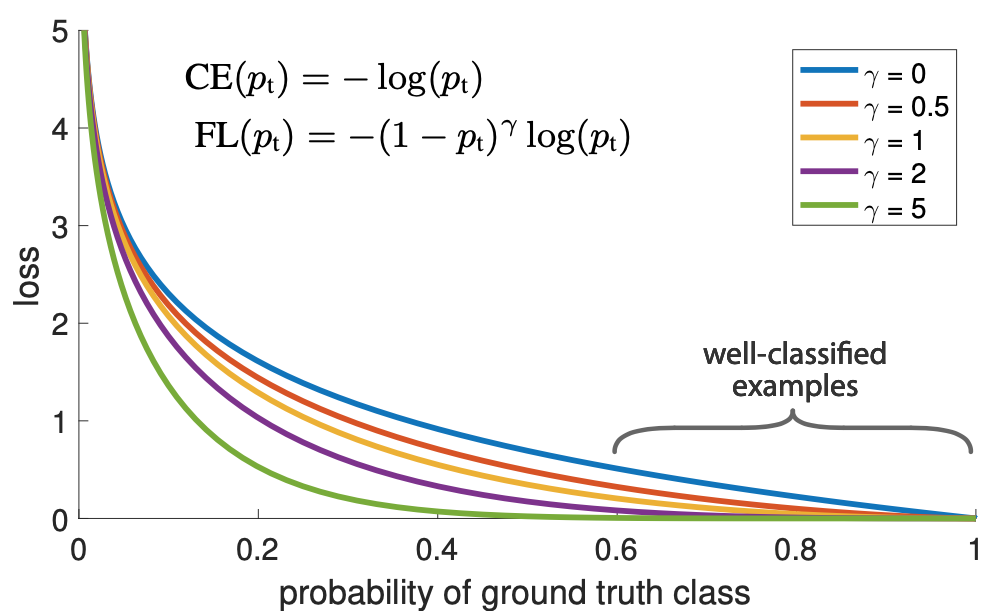
\includegraphics[width=10cm] {images/retinanet_focal_loss_curve}
        \caption{So sánh các tham số của hàm Focal loss với hàm Cross Entropy loss. (Nguồn: \cite{lin2017focal})}
        \label{fig:retinanet_focal_loss_curve}
    \end{figure}

    \noindent
    Ngoài ra, nhóm tác giả còn đề xuất một dạng khác của hàm FL bằng việc sử dụng thêm một tham số $\alpha$ và trong các thí nghiệm, dạng này cho kết quả tốt hơn một chút so với dạng hàm FL không sử dụng $\alpha$.

    \begin{equation}
        FL(p_\textrm{t}) = - \alpha_\textrm{t} (1 - p_\textrm{t})^\gamma \log (p_\textrm{t})
    \end{equation}
    
    \noindent
    \textbf{\textit{Kiến trúc mô hình RetinaNet}} \\
    RetinaNet là mô hình single-stage object detection gồm có các thành phần:
    - Phần \textit{backbone Feature Pyramid Networks} được sử dụng nhằm trích xuất đặc trưng của ảnh đầu vào với nhiều kích thước đặc trưng khác nhau.
    Chi tiết về sức mạnh của FPN đã được thảo luận ở \textit{phần 2.2. Kiến trúc Feature Pyramid Networks}.
    - Phần trích xuất anchor được thực hiện tương tự với cách trích xuất của mô hình RPN biến thể đã phân tích ở \textit{phần 2.2}.
    Tuy nhiên, nhóm tác giả đã thử nghiệm và bổ sung thêm các kích thước $2^{0}$, $2^{1/3}$, $2^{2/3}$ của anchor để đạt kết quả tốt hơn.
    Các anchor được gán groundtruth với chiến lược tương tự như trong \textit{phần 2.1.3. Mô hình Faster R-CNN} nhưng điều chỉnh một số điểm: (1) thay đổi trở thành bài toán multi-class classification (nhóm tác giả của \textit{phần 2.1.3} sử dụng bài toán binary classification phân lớp giữa \textit{anchor có chứa object} và \textit{anchor không chứa object}) và (2) thay đổi threshold IoU để gán nhãn cho từng anchor.

    \begin{figure}[H]
        \centering
        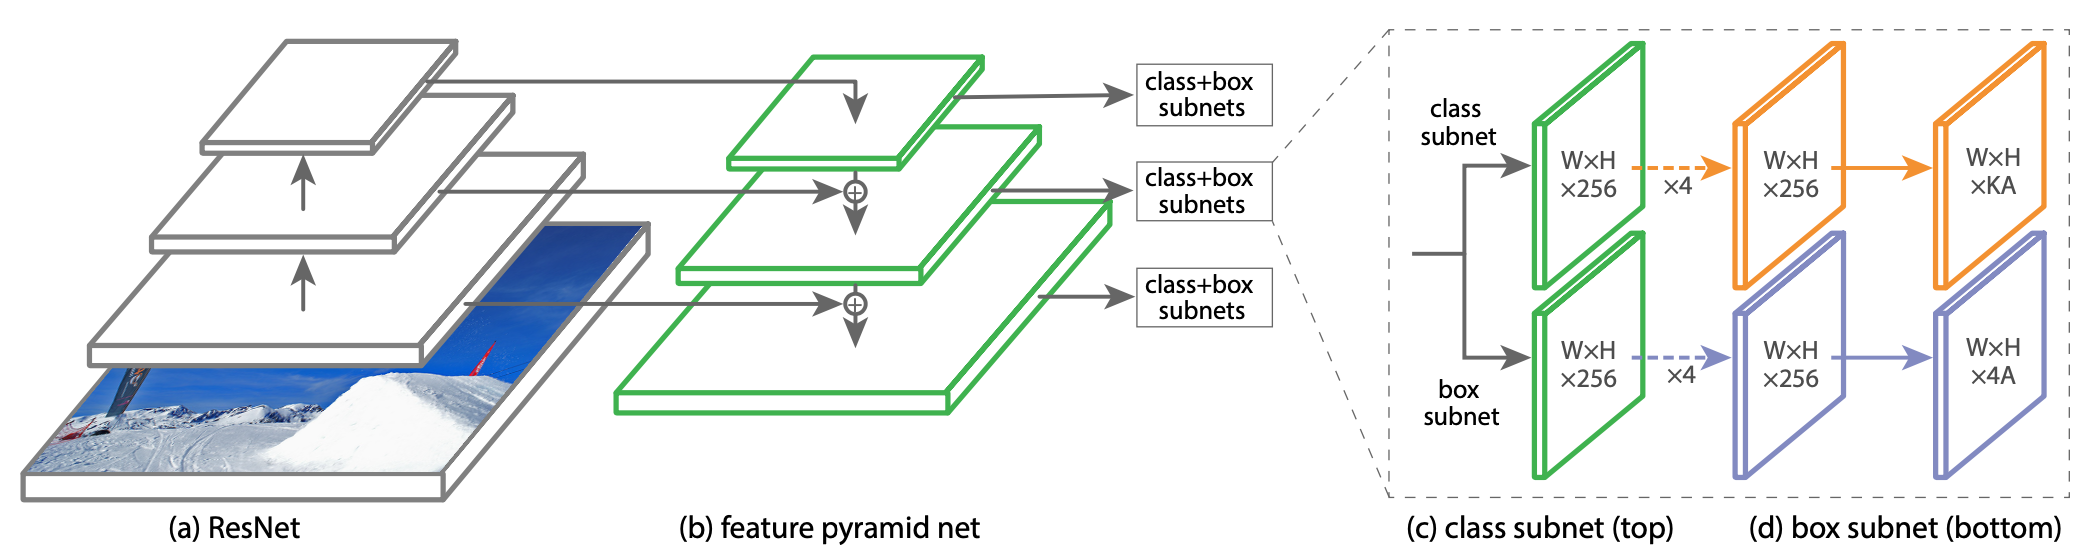
\includegraphics[width=10cm] {images/retinanet_model}
        \caption{Kiến trúc mô hình RetinaNet. (Nguồn: \cite{lin2017focal})}
        \label{fig:retinanet_model}
    \end{figure}

    \noindent
    - Phần \textit{Classification Subnet} được chia sẻ giữa tất cả các feature maps của backbone FPN, gồm các lớp Conv 3x3xC và lớp Conv cuối cùng 3x3xKA.
    Trong đó, K là số lượng lớp đối tượng trong bài toán object detection, A là số lượng anchor tại vị trí trên mỗi feature maps của backbone FPN (tác giả chọn $A = 9$), C là số lượng channel của lớp Conv (tác giả chọn $C = 256$). \\
    - Phần \textit{Box Regression Subnet} được thiết kế khác với cách thiết kế trong mô hình Faster R-CNN khi không dùng chung các lớp Conv với \textit{Classification Subnet}.
    \textit{Box Regression Subnet} cũng gồm các lớp Conv 3x3xC và lớp Conv cuối cùng 3x3x4A.
    Trong đó, A là số lượng anchor tại vị trí trên mỗi feature maps của backbone FPN (tác giả chọn $A = 9$), 4 là 4 độ lệch trong toạ độ của bounding box dự đoán so với groundtruth, C là số lượng channel của lớp Conv (tác giả chọn $C = 256$).

    \noindent
    \textbf{\textit{Kết quả của mô hình RetinaNet}} \\
    Trong thử nghiệm của RetinaNet với các tham số khác nhau của hàm Focal loss, tất cả các cấu hình được train với bộ dữ liệu \textit{COCO trainval135k} và kết quả thu được đánh giá trên bộ dữ liệu \textit{COCO minival}.
    Kết quả của cấu hình $\gamma = 2.0$ và $\alpha = 0.25$ đạt kết quả tốt nhất so với các cấu hình khác của hàm Focal loss.

    \begin{figure}[H]
        \centering
        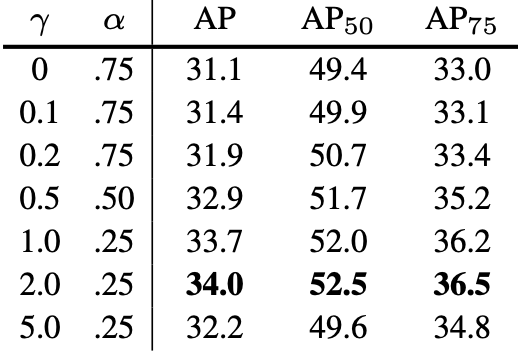
\includegraphics[width=10cm] {images/retinanet_results_2}
        \caption{Kết quả thử nghiệm hàm Focal loss với các tham số khác nhau. (Nguồn: \cite{lin2017focal})}
        \label{fig:retinanet_results_2}
    \end{figure}

    Khi so sánh kết quả của mô hình RetinaNet với các mô hình object detection khác vào thời điểm đó, kết quả của các cấu hình khác nhau của mô hình RetinaNet cũng đạt kết quả rất tốt về cả tốc độ lẫn độ chính xác của mô hình.
    Cụ thể các mô hình được so sánh gồm: \\
    - Kết quả của mô hình YOLOv2 ký hiệu là [A] \cite{redmon2016yolo9000} (Kết quả không được biểu diễn trên hình) \\
    - Kết quả của mô hình SSD321, ký hiệu là [B] \cite{liu2016ssd} \\
    - Kết quả của mô hình DSSD321, ký hiệu là [C] \cite{fu2017dssd} \\
    - Kết quả của mô hình R-FCN, ký hiệu là [D] \cite{dai2016r} \\
    - Kết quả của mô hình SSD513, ký hiệu là [E] \cite{liu2016ssd} \\
    - Kết quả của mô hình DSSD513, ký hiệu là [F] \cite{fu2017dssd} \\
    - Kết quả của mô hình FPN FRCN, ký hiệu là [G] \cite{lin2017feature} \\
    - Kết quả của mô hình RetinaNet sử dụng backbone là ResNet50 và sử dụng ảnh đầu vào có kích thước 500 pixel, ký hiệu là RetinaNet-50-500. \\
    - Kết quả của mô hình RetinaNet sử dụng backbone là ResNet101 và sử dụng ảnh đầu vào có kích thước 500 pixel, ký hiệu là RetinaNet-101-500 \\
    - Kết quả của mô hình RetinaNet sử dụng backbone là ResNet101 và sử dụng ảnh đầu vào có kích thước 800 pixel, ký hiệu là RetinaNet-101-800 \\
    Đường màu xanh và màu cam trên hình lần lượt là các cấu hình RetinaNet sử dụng backbone ResNet50 và ResNet101 và với các cấu hình ảnh đầu vào từ 400 pixel đến 800 pixel.

    \begin{figure}[H]
        \centering
        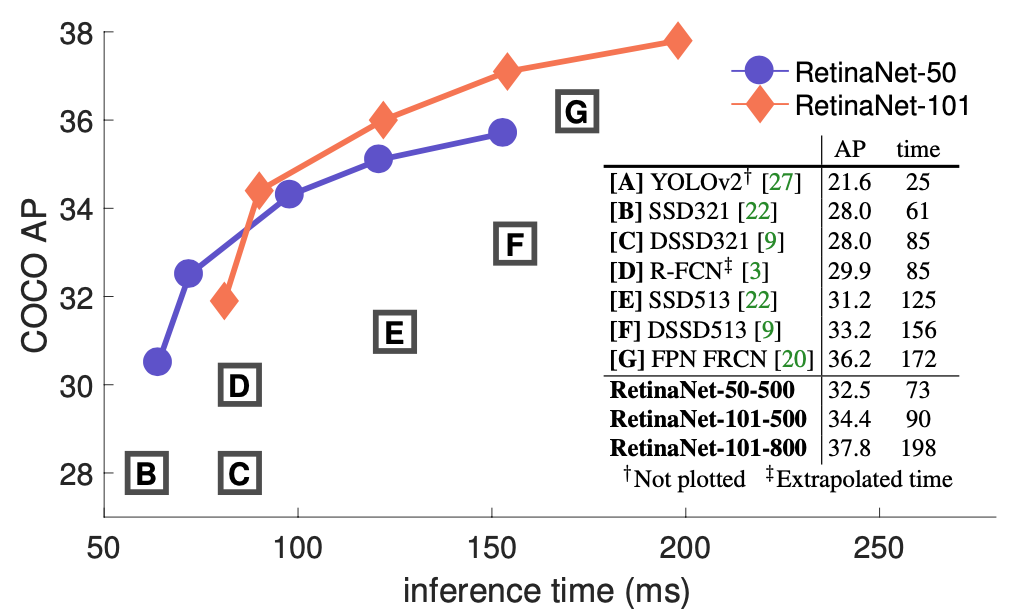
\includegraphics[width=6cm] {images/retinanet_results_1}
        \caption{So sánh kết quả mô hình RetinaNet với một số mô hình object detection khác. (Nguồn: \cite{lin2017focal})}
        \label{fig:retinanet_results_1}
    \end{figure}

    Kết quả, các cấu hình khác nhau của RetinaNet đều cho kết quả tốt hơn so với các mô hình object detection khác (cả single-stage và two-stage).
    So với mô hình đạt độ chính xác tốt nhất ở thời điểm đó là [G], cấu hình RetinaNet-101-700 cho kết quả chính xác hơn với thời gian nhanh hơn.
    So với các mô hình đạt tốc độ tốt nhất ở thời điểm đó là [A] và [B], cấu hình RetinaNet-50-400 cho kết quả chậm hơn nhưng với độ chính xác cao hơn vượt trội.

    \noindent
    \textbf{\textit{Kết luận về mô hình RetinaNet}} \\
    Mô hình RetinaNet ra đời là một bước tiến lớn đối với việc giải quyết bài toán object detection khi nó giải quyết vấn đề mất cân bằng dữ liệu của các mô hình single-stage giúp tăng độ chính xác của mô hình ngang bằng với các mô hình two-stage nhưng vẫn duy trì được một tốc độ nhanh và có thể sử dụng trong thời gian thực. \\
    Mô hình RetinaNet cho đến nay vẫn là một mô hình tốt để giải quyết các bài toán con của object detection, cụ thể là face detection.
    Trong các phần tiếp theo của luận văn, ta sẽ bàn luận về các mô hình kế thừa RetinaNet giải quyết rất tốt bài toán face detection.
}
    \retinanet

    \subsection{Mô hình AutoFocus}
    \def\autofocus{
    Từ vấn đề tồn đọng của phương pháp chuẩn bị dữ liệu SNIPER, mô hình AutoFocus \cite{najibi2019autofocus} đã ra đời nhằm tăng tốc quá trình dự đoán của mô hình nhận diện đối tượng.
    AutoFocus hướng đến việc loại bỏ những pixel dư thừa mà mô hình phải xử lý trong quá trình dự đoán nhưng vẫn giữ được ý tưởng về việc sử dụng Image Pyramids.
    Mô hình AutoFocus được thiết kế nhằm dự đoán những khu vực đáng chú ý ở trên ảnh và loại bỏ những khu vực khả năng cao không chứa đối tượng ở những kích thước ảnh lớn hơn.
    Từ đó, tiết kiệm được rất nhiều chi phí tính toán trong quá trình predict của mô hình.

    \noindent
    \textbf{\textit{Kiến trúc tổng quá của mô hình AutoFocus}} \\
    Mô hình AutoFocus gồm hai nhánh: \\
    - Nhánh Focus (cụ thể gọi là Nhánh Focus Pixel Prediction) là nhánh mô hình giúp xác định được khu vực đáng chú ý trên ảnh để zoom to hơn, đồng thời loại bỏ các khu vực khả năng cao không chứa đối tượng. \\
    - Nhánh Detection là nhánh giúp mô hình định vị chính xác bounding box của từng đối tượng.
    Trong nghiên cứu, nhóm tác giả sử dụng mô hình Faster R-CNN \cite{ren2015faster} làm cơ sở cho nhánh Detection.

    \begin{figure}[H]
        \centering
        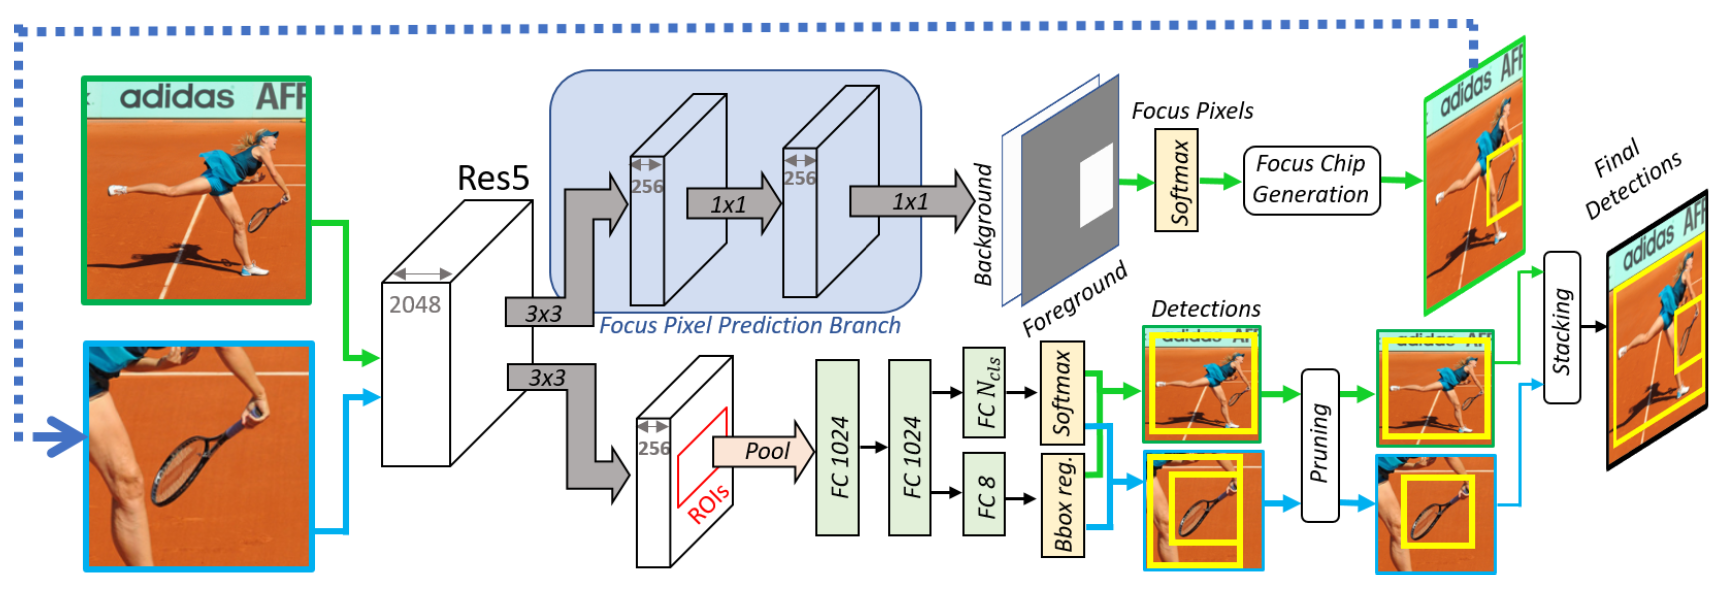
\includegraphics[width=15cm] {images/autofocus_model}
        \caption{Kiến trúc mô hình AutoFocus (Nguồn: \cite{najibi2019autofocus})}
        \label{fig:autofocus_model}
    \end{figure}
    
    \noindent
    Mô hình này nhận đầu vào xuất phát từ ảnh có kích thước nhỏ với mục tiêu định vị được những đối tượng có kích thước lớn và xác định khu vực khả năng cao chứa đối tượng.
    Với các khu vực khả năng cao chứa đối tượng, AutoFocus tiếp tục zoom vào với kích thước lớn hơn nhằm định vị được những đối tượng có kích thước nhỏ hơn và tiếp tục xác định khu vực khả năng cao chứa đối tượng.
    Quá trình này sẽ lặp đi lặp lại cho đến khi không còn khu vực nào cần phải zoom thì thuật toán sẽ dừng lại. \\
    Mô hình AutoFocus gồm ba thành phần là \textit{Thuật toán Focus Pixel} và \textit{Thuật toán sinh Focus Chips} thuộc nhánh Focus và \textit{Thuật toán Focus Stacking} thuộc nhánh Detection.

    \noindent
    \textbf{\textit{Thuật toán Focus Pixel}} \\
    Thuật toán Focus Pixel là thuật toán giúp chúng ta có thể xác định được vị trí khu vực có khả năng chứa đối tượng và cần zoom trên ảnh.
    Ý tưởng của thuật toán Focus Pixel dựa trên việc khi ta đưa đầu vào một ảnh có kích thước $X \times Y$ qua một khối Conv (như trong mô hình ResNet), feature maps mà ta thu được có kích thước $X' \times Y'$, trong đó: $X' = \lceil \frac{X}{s} \rceil$, $Y' = \lceil \frac{Y}{s} \rceil$, và $s$ là stride của cả khối Conv.
    Từ đó ta có thể ngầm hiểu rằng một pixel trên feature maps có kích thước $X' \times Y'$ đại diện cho một khu vực có kích thước $s \times s$ trên ảnh đầu vào. \\
    Với ý tưởng trên, từ groundtruth bounding box của đối tượng trên ảnh đầu vào, thuật toán Focus Pixel giúp xây dựng được label dạng mask của nhánh Focus với kích thước chiều dài chiều rộng bằng với khối Conv5 của mô hình backbone ResNet. \\
    Cụ thể hơn, Focus Pixel xác định các pixel trên mask là các \textit{pixel cần được focus} nếu như pixel đó có overlap với grountruth bounding box của đối tượng có kích thước nhỏ.
    Tiếp theo, các pixel trên mask là các \textit{pixel không cần quan tâm} nếu như pixel đó có overlap với groundtruth bounding box của đối tượng có kích thước lớn hoặc rất nhỏ.
    Cuối cùng, các \textit{pixel không cần được focus} trên mask là các pixel còn lại.

    \[l = 
        \begin{cases}
            1, & IoU(GT, l) > 0, a < \sqrt{GTArea} < b \\
            -1, & IoU(GT, l) > 0, \sqrt{GTArea} < a  \\
            -1, & IoU(GT, l) > 0, b < \sqrt{GTArea} < c  \\
            0, & \text{otherwise}
        \end{cases}
    \]

    \noindent
    trong đó: \\
    - $IoU(GT, l)$ là chỉ số IoU giữa khu vực $s \times s$ và groundtruth bounding box của đối tượng trên ảnh đầu vào. \\
    - $GTArea$ là diện tích của groundtruth bounding box của đối tượng trên ảnh đầu vào. \\
    Nếu một khu vực $s \times s$ overlap với nhiều groundtruth bounding box của đối tượng, thì pixel đó được ưu tiên là một Focus Pixel.

    \begin{figure}[H]
        \centering
        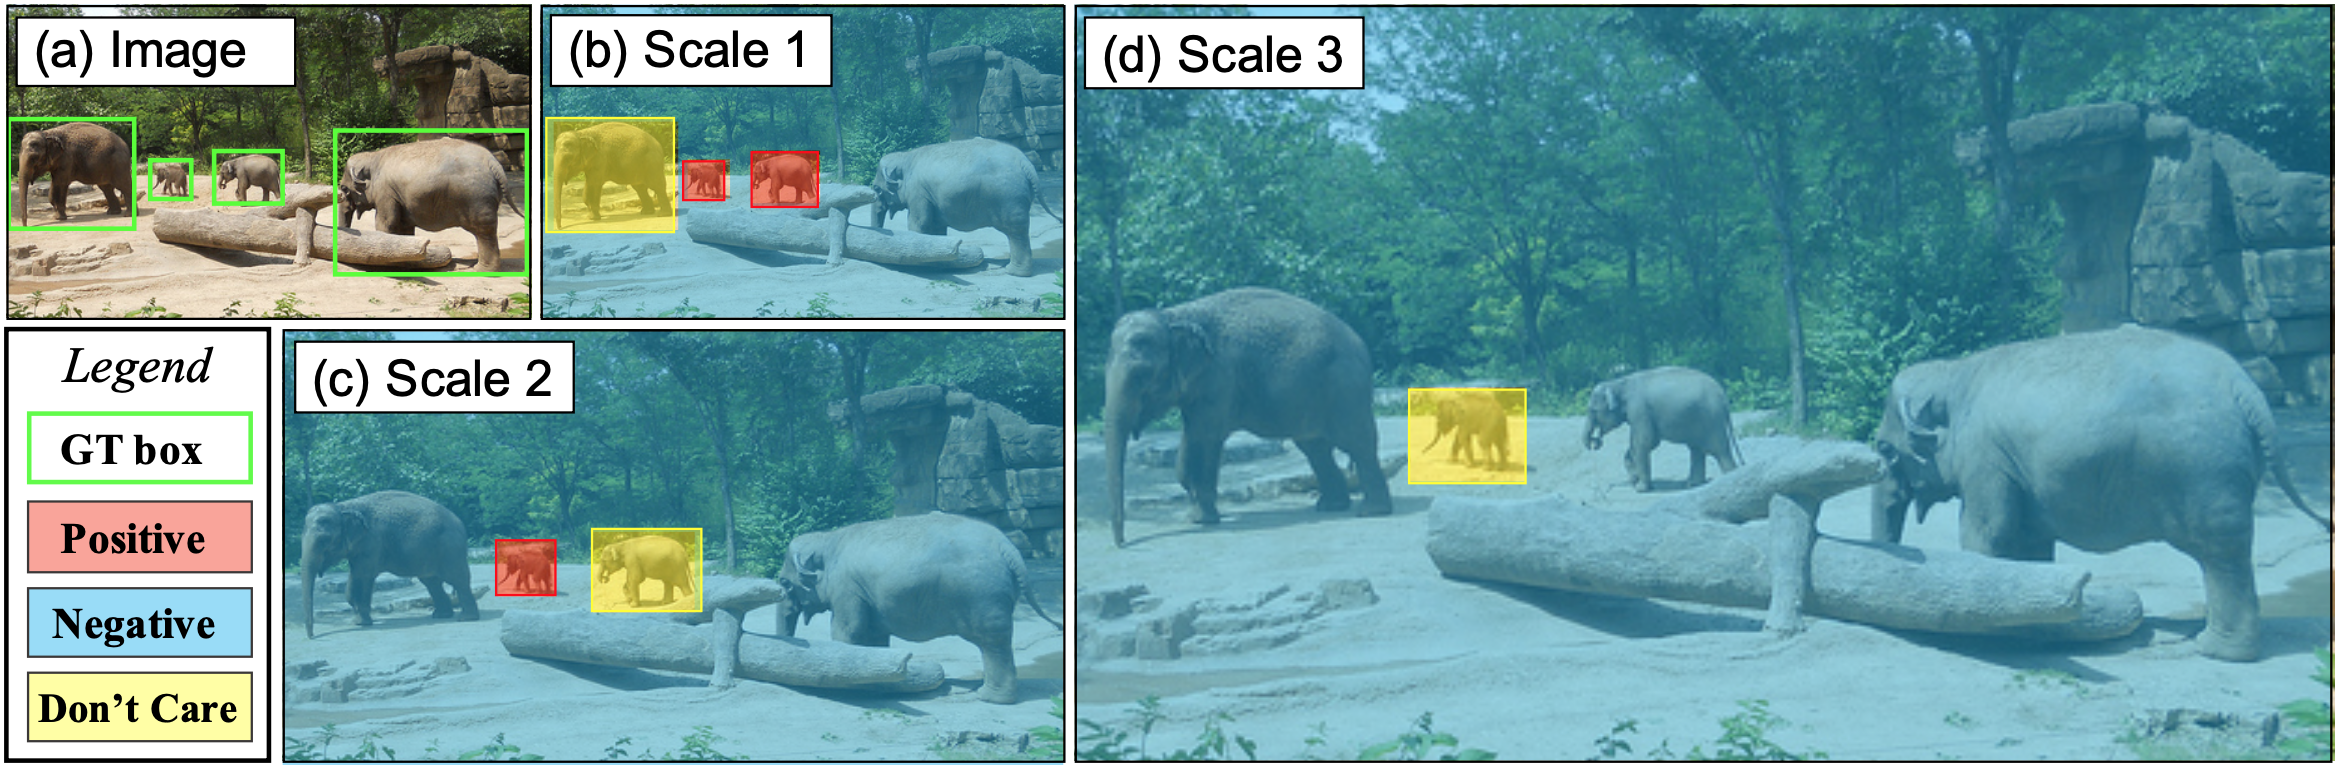
\includegraphics[width=15cm] {images/autofocus_focus_pixel}
        \caption{Ví dụ về cơ chế hoạt động của thuật toán Focus Pixel (Nguồn: \cite{najibi2019autofocus})}
        \label{fig:autofocus_focus_pixel}
    \end{figure}

    \noindent
    Trong các thí nghiệm mà nhóm tác giả thực hiện trong nghiên cứu, nhóm tác giả sử dụng ảnh đầu vào có kích thước $512 \times 512$, với các tham số $a = 5, b = 64, c = 90$ nghĩa là các groundtruth bounding box có kích thước từ $5 \times 5$ đến $64 \times 64$ là các bounding box cần được focus, các groundtruth bounding box có kích thước dưới $5 \times 5$ hoặc từ $64 \times 64$ đến $90 \times 90$ là các bounding box không cần quan tâm và các groundtruth bounding box có kích thước trên $90 \times 90$ là các bounding box không cần được focus.
    Từ các tham số trên, tỷ lệ giữa các \textit{pixel cần được focus} và \textit{pixel không cần được focus} là 10.

    \noindent
    \textbf{\textit{Thuật toán sinh Focus Chips}} \\
    Sau khi mô hình đã được train và predict ra được pixel cần được focus, mô hình cần một thuật toán để crop ra được khu vực cần focus trên ảnh làm đầu vào cho mô hình AutoFocus lượt tiếp theo.
    Và đó là vai trò của thuật toán sinh Focus Chips.

    \begin{figure}[H]
        \centering
        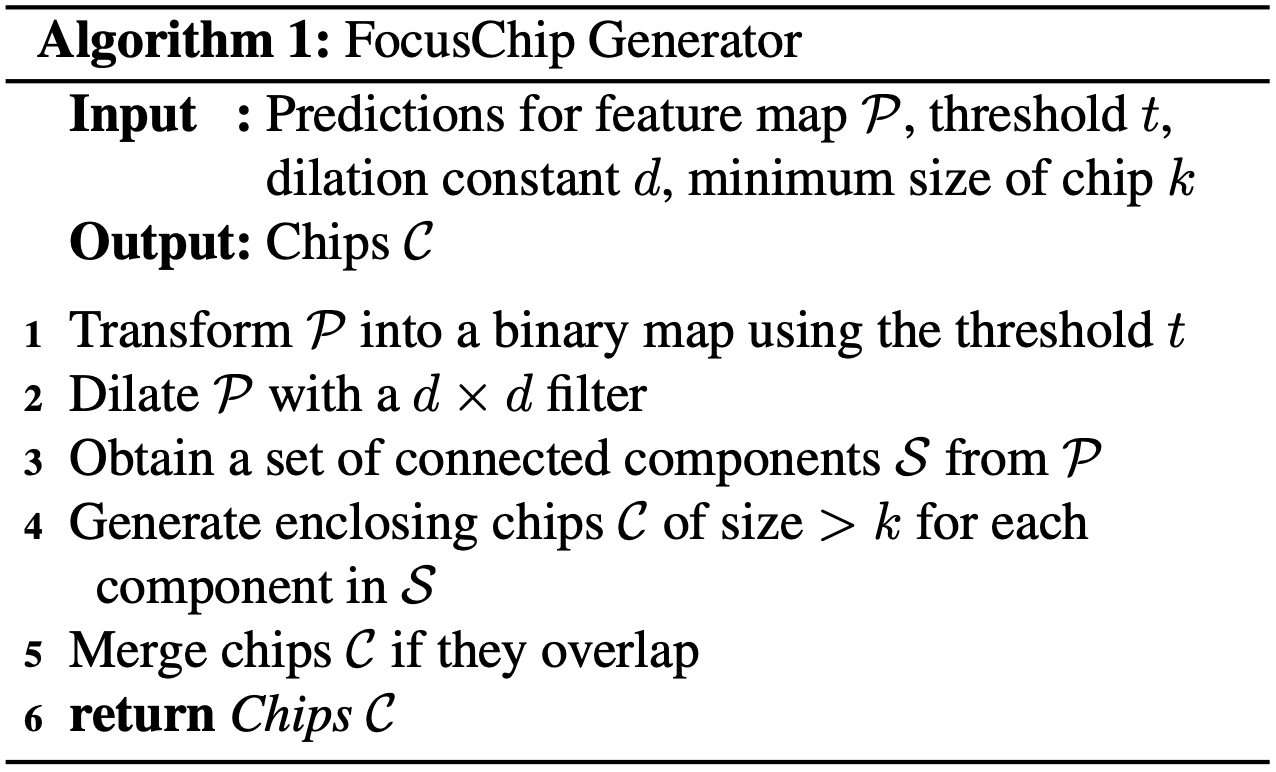
\includegraphics[width=10cm] {images/autofocus_focus_chip_gen}
        \caption{Chi tiết thuật toán sinh Focus Chips (Nguồn: \cite{najibi2019autofocus})}
        \label{fig:autofocus_focus_chip_gen}
    \end{figure}

    \noindent
    Trong quá trình predict, sau khi mô hình đã predict được các pixel cần được focus (ký hiệu là $\mathcal{P}$) trên Focus Pixel mask, ta biến đổi mask này trở về dạng binary mask bằng threshold $t$.
    Tham số $t$ được sử dụng để cân đối giữa tốc độ và độ chính xác của mô hình (cụ thể với tham số $t$ lớn, số lượng các pixel cần được focus sẽ giảm đi và tốc độ của mô hình AutoFocus sẽ tăng và ngược lại). \\
    Từ binary mask đã được sinh ra ở trên, thuật toán sinh Focus Chips sẽ đưa qua một filter có kích thước $d \times d$ nhằm giãn nở các pixel thêm một chút để thu được các thành phần liên thông $\mathcal{S}$, từ đó có nhiều thông tin hơn khi crop ảnh đầu vào với các focus pixel này. \\
    Cuối cùng, ta crop ra các chip $\mathcal{C}$ với kích thước tối thiểu là $k \times k$ và bao trọn các thành phần liên thông $\mathcal{S}$ trên.
    Các chip trong $\mathcal{C}$ nếu có overlap với nhau sẽ được gộp lại chung thành một chip. \\
    Việc sinh ra các chip $\mathcal{C}$ giúp mô hình AutoFocus có thể sử dụng ý tưởng Image Pyramids nhưng tiết kiệm chi phí tính toán nhờ loại bỏ các khu vực khả năng cao không chứa đối tượng.

    \noindent
    \textbf{\textit{Thuật toán Focus Stacking}} \\
    Một vấn đề cần phải giải quyết khi thực hiện predict với ý tưởng Image Pyramids trong bài toán nhận diện đối tượng là việc tổng hợp lại các bounding box.
    Đối với mô hình AutoFocus, vấn đề này còn phức tạp hơn với trường hợp một đối tượng có kích thước lớn được dự đoán ở kích thước này, nhưng đến kích thước tiếp theo, đối tượng đó bị crop trong quá trình crop chip và trở thành một đối tượng có kích thước nhỏ hơn.
    Nhằm hạn chế bớt vấn đề này, nhóm tác giả chỉ ra rằng \textit{bước 2} trong thuật toán sinh Focus Chips \ref{fig:autofocus_focus_chip_gen} là cực kỳ quan trọng.

    \begin{figure}[H]
        \centering
        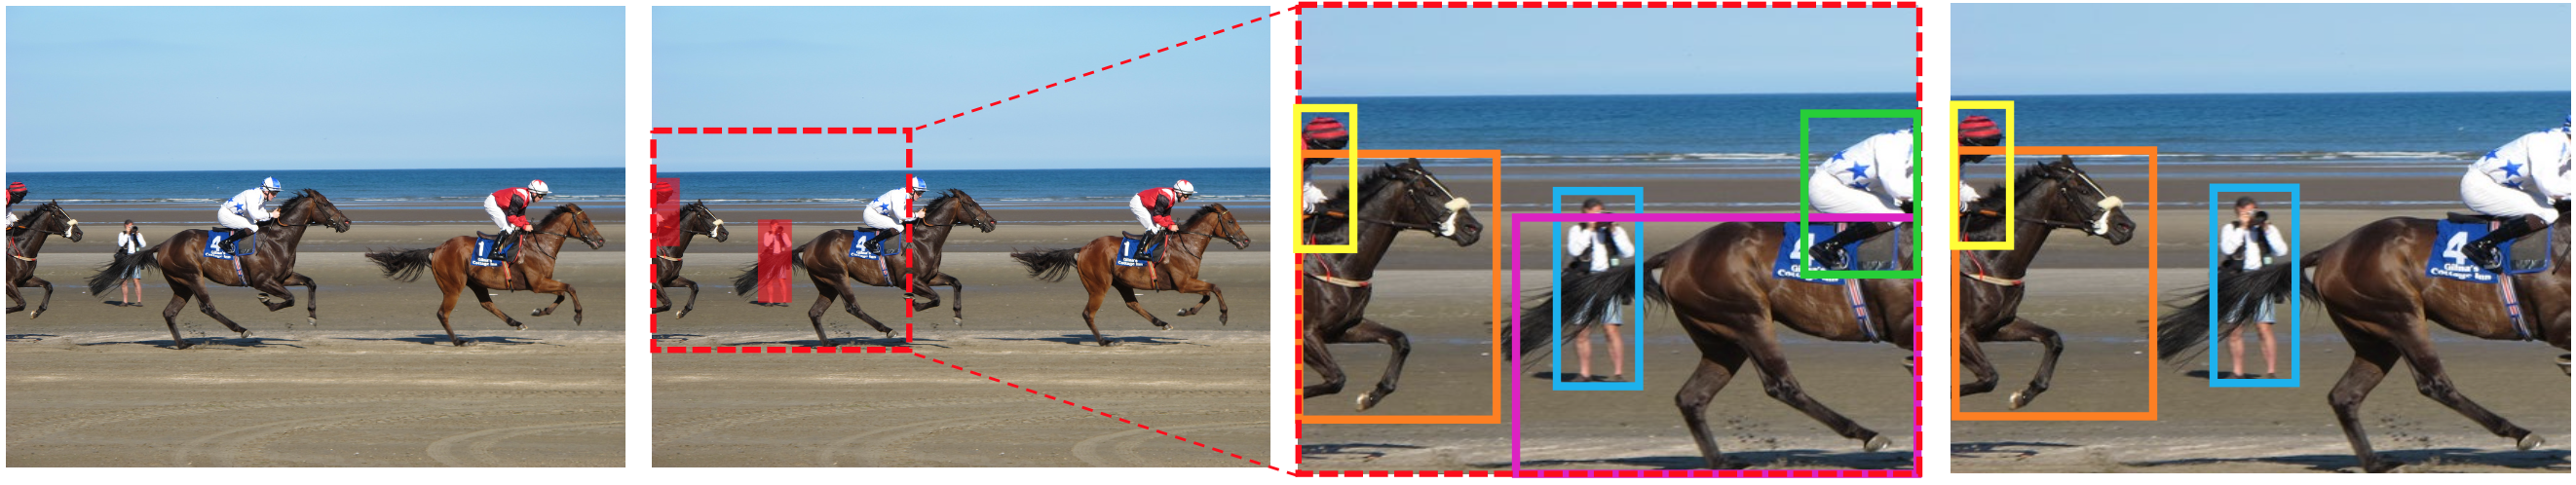
\includegraphics[width=10cm] {images/autofocus_focus_stack}
        \caption{Ví dụ về cơ chế hoạt động của thuật toán Focus Stacking (Nguồn: \cite{najibi2019autofocus})}
        \label{fig:autofocus_focus_stack}
    \end{figure}

    \noindent
    Tuy nhiên, nhóm tác giả cũng đề ra một số luật nhằm loại bỏ các dự đoán lỗi của các đối tượng được định vị trên một focus chip: \\
    - Nếu một đối tượng nằm trên một biên của chip nhưng không phải biên của ảnh đầu vào (nghĩa là đối tượng này đã bị crop sau khi qua thuật toán sinh Focus Chip), thì dự đoán sẽ bị loại bỏ. \\
    - Nếu một đối tượng nằm trên một biên của chip và đó là biên của ảnh đầu vào, nhóm tác giả sẽ tiếp tục kiểm tra biên còn lại của đối tượng, nếu đó là biên của chip, dự đoán sẽ bị loại, còn nếu đó không phải là biên của chip, dự đoán sẽ được giữ lại. \\
    - Nếu một đối tượng nằm trên hai biên của chip và đó đều là hai biên của ảnh đầu vào, nhóm tác giả sẽ giữ lại những dự đoán này. \\
    Sau khi loại bỏ bớt các dự đoán bằng thuật toán Focus Stacking, mô hình AutoFocus đưa ra tổng hợp dự đoán từ các kích thước ảnh khác nhau và là các dự đoán cuối cùng của ảnh đầu vào.

    \noindent
    \textbf{\textit{Kết quả của mô hình AutoFocus}} \\
    Kết quả của mô hình AutoFocus so sánh với các mô hình khác là rất ấn tượng trên bộ dữ liệu COCO test-dev.
    Số lượng pixel mà mô hình cần xử lý được chú thích tại cột \textit{Pixels}.
    Mô hình AutoFocus giữ được kết quả tương đương với mô hình sử dụng phương pháp chuẩn bị dữ liệu SNIPER trên tất cả các chỉ số trong khi đạt số lượng pixel cần xử lý ít hơn nhiều so với mô hình sử dụng SNIPER.

    \begin{figure}[H]
        \centering
        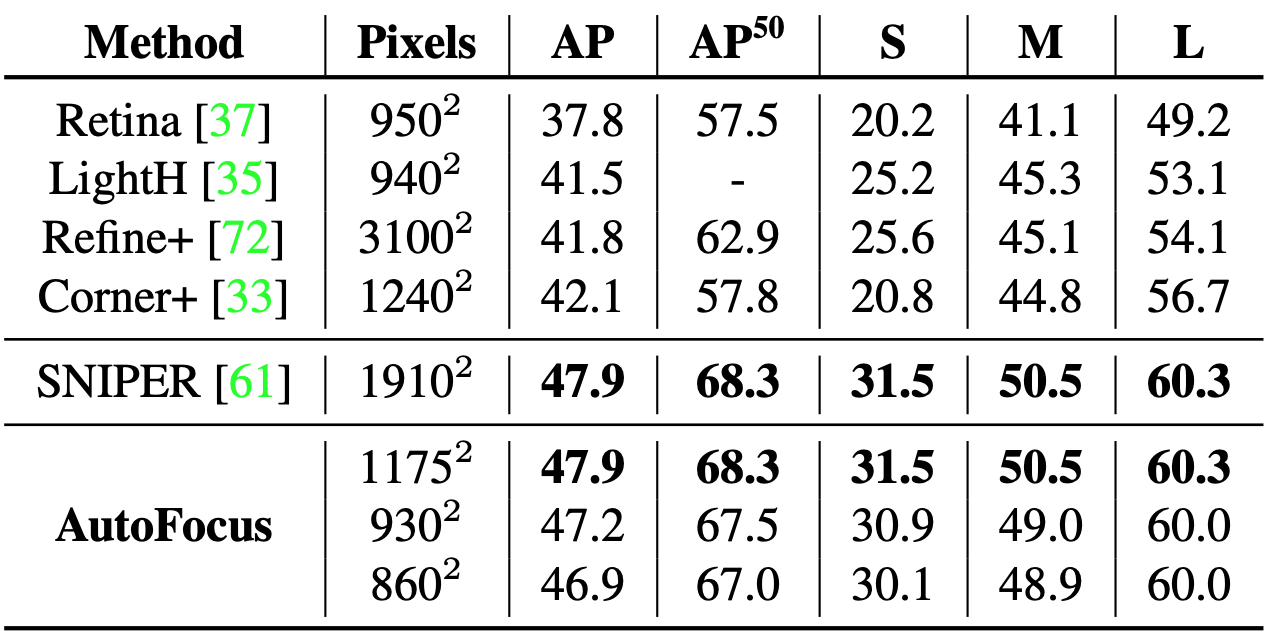
\includegraphics[width=10cm] {images/autofocus_results_1}
        \caption{Kết quả của mô hình AutoFocus so sánh với các mô hình khác trên bộ dữ liệu COCO test-dev (Nguồn: \cite{najibi2019autofocus})}
        \label{fig:autofocus_results_1}
    \end{figure}

    \noindent
    Nhóm tác giả chia sẻ rằng dù đạt kết quả là 47.9\% tương đương với SNIPER, nhưng AutoFocus có khả năng xử lý khoảng 6.4 ảnh/giây trên bộ COCO test-dev trên Titan X Pascal GPU so sánh với chỉ 2.5 ảnh/giây của mô hình sử dụng SNIPER. \\
    Mô hình RetinaNet với ResNet-101 backbone đạt tốc độ gần tương đương với AutoFocus là 6.4 ảnh/giây trên bộ COCO test-dev trên P100 GPU (tương đương với Titan X Pascal GPU) nhưng chỉ đạt mức mAP là 37.8\%.
    Nhóm tác giả cũng nhấn mạnh rằng AutoFocus là mô hình nhanh nhất ở thời điểm đó xử lý bộ dữ liệu COCO và đạt chỉ số mAP là 47.9\%.

    \begin{figure}[H]
        \centering
        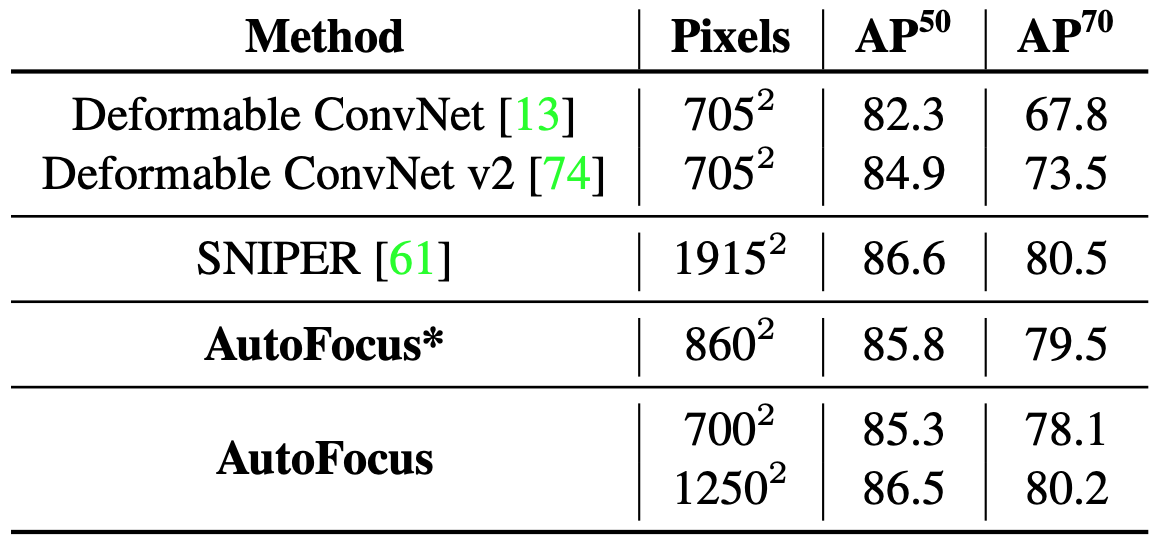
\includegraphics[width=10cm] {images/autofocus_results_2}
        \caption{Kết quả của mô hình AutoFocus so sánh với các mô hình khác trên bộ dữ liệu PASCAL VOC 2007 test-set (Nguồn: \cite{najibi2019autofocus})}
        \label{fig:autofocus_results_2}
    \end{figure}

    \noindent
    Kết quả của mô hình AutoFocus so sánh với các mô hình khác trên bộ dữ liệu PASCAL VOC 2007 test-set cũng được nhóm tác giả chia sẻ.
    Ở đây, nhóm tác giả cũng nhấn mạnh vào sức mạnh của mô hình AutoFocus khi sử dụng cấu hình được finetune của mô hình trên bộ dữ liệu COCO (mô hình ký hiệu là AutoFocus*) để giải quyết bộ dữ liệu PASCAL VOC 2007 nhưng vẫn đạt kết quả tốt.

    \begin{figure}[H]
        \centering
        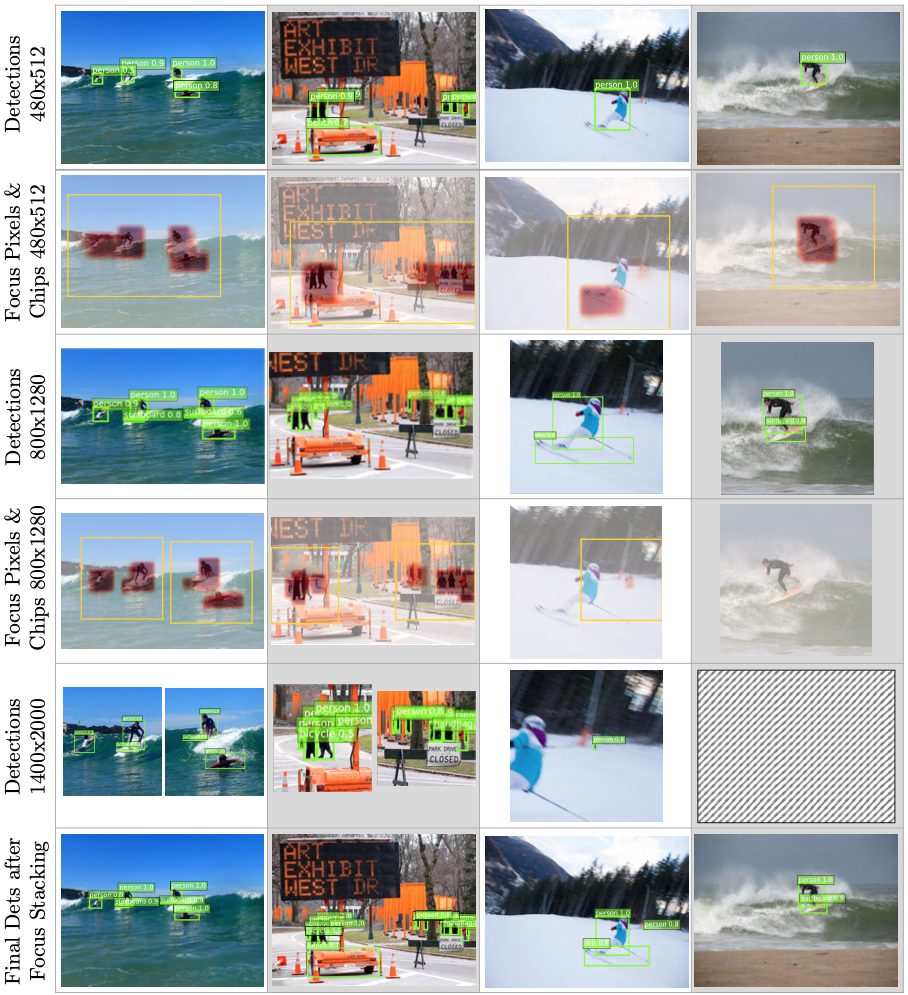
\includegraphics[width=10cm] {images/autofocus_results_3}
        \caption{Từng bước quá trình dự đoán của mô hình AutoFocus với một số ảnh trong bộ dữ liệu COCO val-2017(Nguồn: \cite{najibi2019autofocus})}
        \label{fig:autofocus_results_3}
    \end{figure}

    \noindent
    \textbf{\textit{Vấn đề tồn đọng của mô hình AutoFocus}} \\
    Nghiên cứu của mô hình AutoFocus đã mang lại một ý tưởng rất thông minh để xử lý rất nhanh bài toán nhận diện đối tượng với ảnh chất lượng cao trong khi vẫn duy trì được độ chính xác cao, tương đương với các mô hình sử dụng phương pháp Image Pyramids truyền thống.
    Tuy nhiên, mô hình AutoFocus vẫn tồn tại điểm yếu khá lớn là số lượng hyperpameter của mô hình nhiều.
    Điều này gây ra khó khăn trong việc tìm kiếm một cấu hình tốt nhất của mô hình đối với từng bài toán hay từng bộ dữ liệu khác nhau.
    Nghiên cứu và phân tích về điểm yếu này sẽ được trình bày trong phần sau của luận văn.
}
    \autofocus

    \subsection{Mô hình RetinaFace}
    \def\retinaface{
    Mô hình RetinaFace \cite{deng2020retinaface} là một mô hình single-stage giải quyết bài toán face detection đạt kết quả tốt trên bộ dữ liệu WIDER FACE \cite{yang2016wider}.
    Mô hình RetinaFace được nhóm tác giả tích hợp nhiều mô hình và kỹ thuật khác nhau giúp nâng cao độ chính xác của mô hình.
    Ngoài ra, với việc sử dụng một mô hình backbone nhỏ hơn là Mobile-Net, mô hình RetinaFace có thể đạt tốc độ chạy trong thời gian thực trên CPU.

    \noindent
    \textbf{\textit{Kiến trúc mô hình RetinaFace}} \\
    Mô hình RetinaFace có kiến trúc dựa trên ý tưởng của RetinaNet \cite{lin2017focal} đã được thảo luận ở \textit{phần 2.3} của luận văn.
    RetinaFace cũng sử dụng kiến trúc backbone Feature Pyramids Network nhằm trích xuất đặc trưng của ảnh đầu vào với nhiều kích thước feature maps khác nhau.
    Tuy nhiên, thay vì sử dụng trực tiếp các feature maps này nhằm trả đầu ra là các bounding box chứa khuôn mặt, RetinaFace đưa các feature maps này qua các khối Context Module nhằm thu thập thêm các thông tin về background xung quanh trước khi đưa ra dự đoán về bounding box.
    
    \begin{figure}[H]
        \centering
        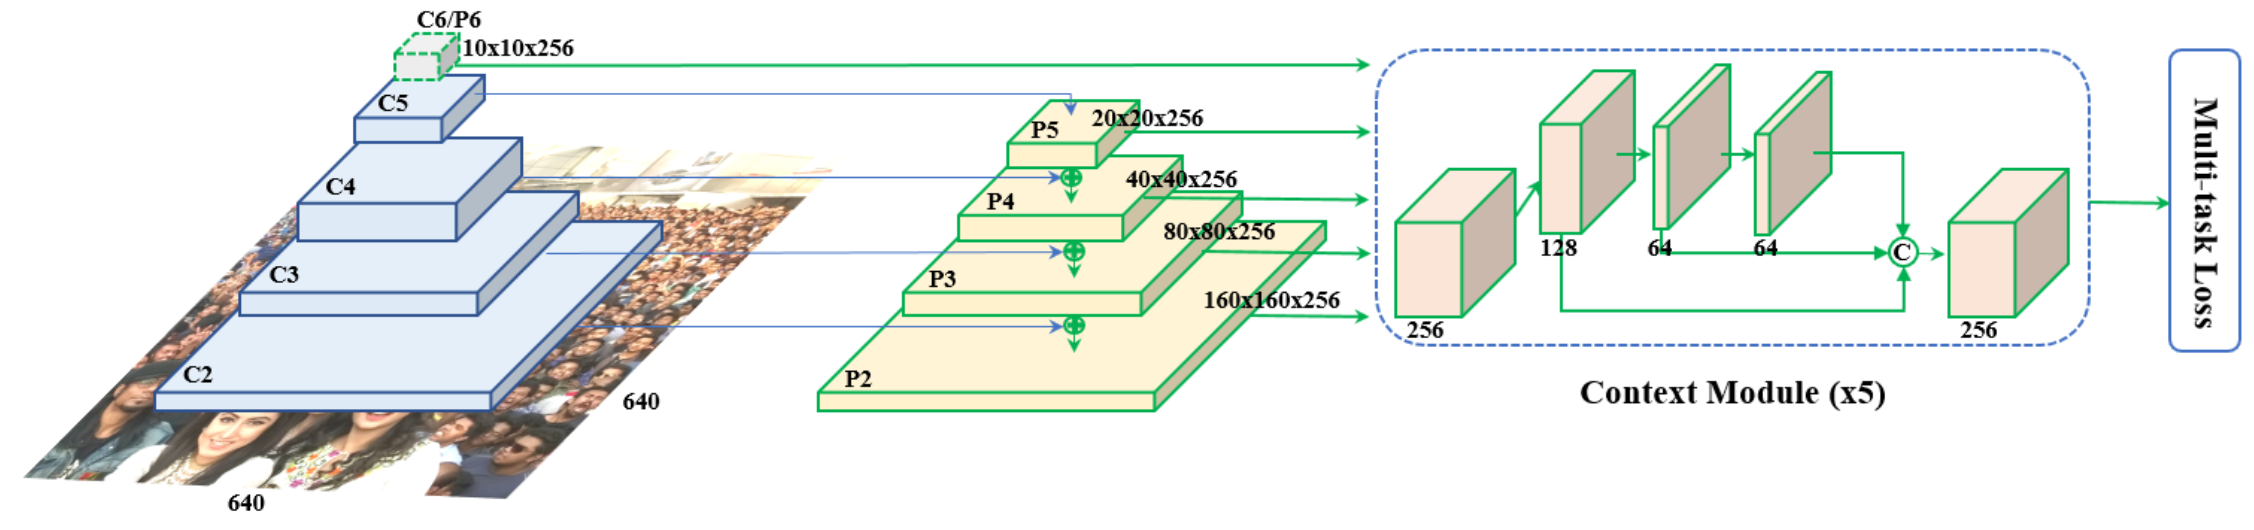
\includegraphics[width=10cm] {images/retinaface_architecture}
        \caption{Kiến trúc của mô hình RetinaFace. (Nguồn: \cite{deng2020retinaface})}
        \label{fig:retinaface_architecture}
    \end{figure}
    
    \noindent
    Ý tưởng sử dụng các khối Context Module tỏ ra khá hiệu quả khi áp dụng với bài toán face detection.
    Đặc biệt trong việc định vị các mặt nhỏ, vì khi những thông tin về background xung quanh như thân người sẽ có vai trò quan trọng giúp mô hình học tốt hơn.
    Trong kiến trúc mô hình RetinaFace, bốn feature maps \textit{{${P}_{2}, {P}_{3}, {P}_{4}, {P}_{5}$}} của FPN và một feature maps \textit{{${C}_{6}$}} của backbone được đưa qua năm khối Context Module độc lập.
    Mỗi khối Context Module gồm ba khối Conv nối tiếp nhau, nhưng feature maps đầu ra của mỗi khối Conv đều được concat lại với nhau để tạo ra feature maps cuối cùng của cả khối Context Module.
    Trong thực tế, nhằm đạt kết quả tốt nhất trên bộ dữ liệu WIDER FACE, mô hình RetinaFace sử dụng kỹ thuật \textit{deformable convolution network} (gọi tắt là DCN) thay thế cho các lớp Conv truyền thống.

    \noindent
    \textbf{\textit{Hệ thống các hàm loss của mô hình RetinaFace}} \\
    Việc nhóm tác giả đã bổ sung thêm landmarks của các khuôn mặt trên bộ WIDER FACE (đã được nhắc đến tại \textit{phần 4.1} của luận văn) đã giúp mô hình RetinaFace có thể xây dựng và tối ưu hàm loss multi-task.

    \begin{figure}[H]
        \centering
        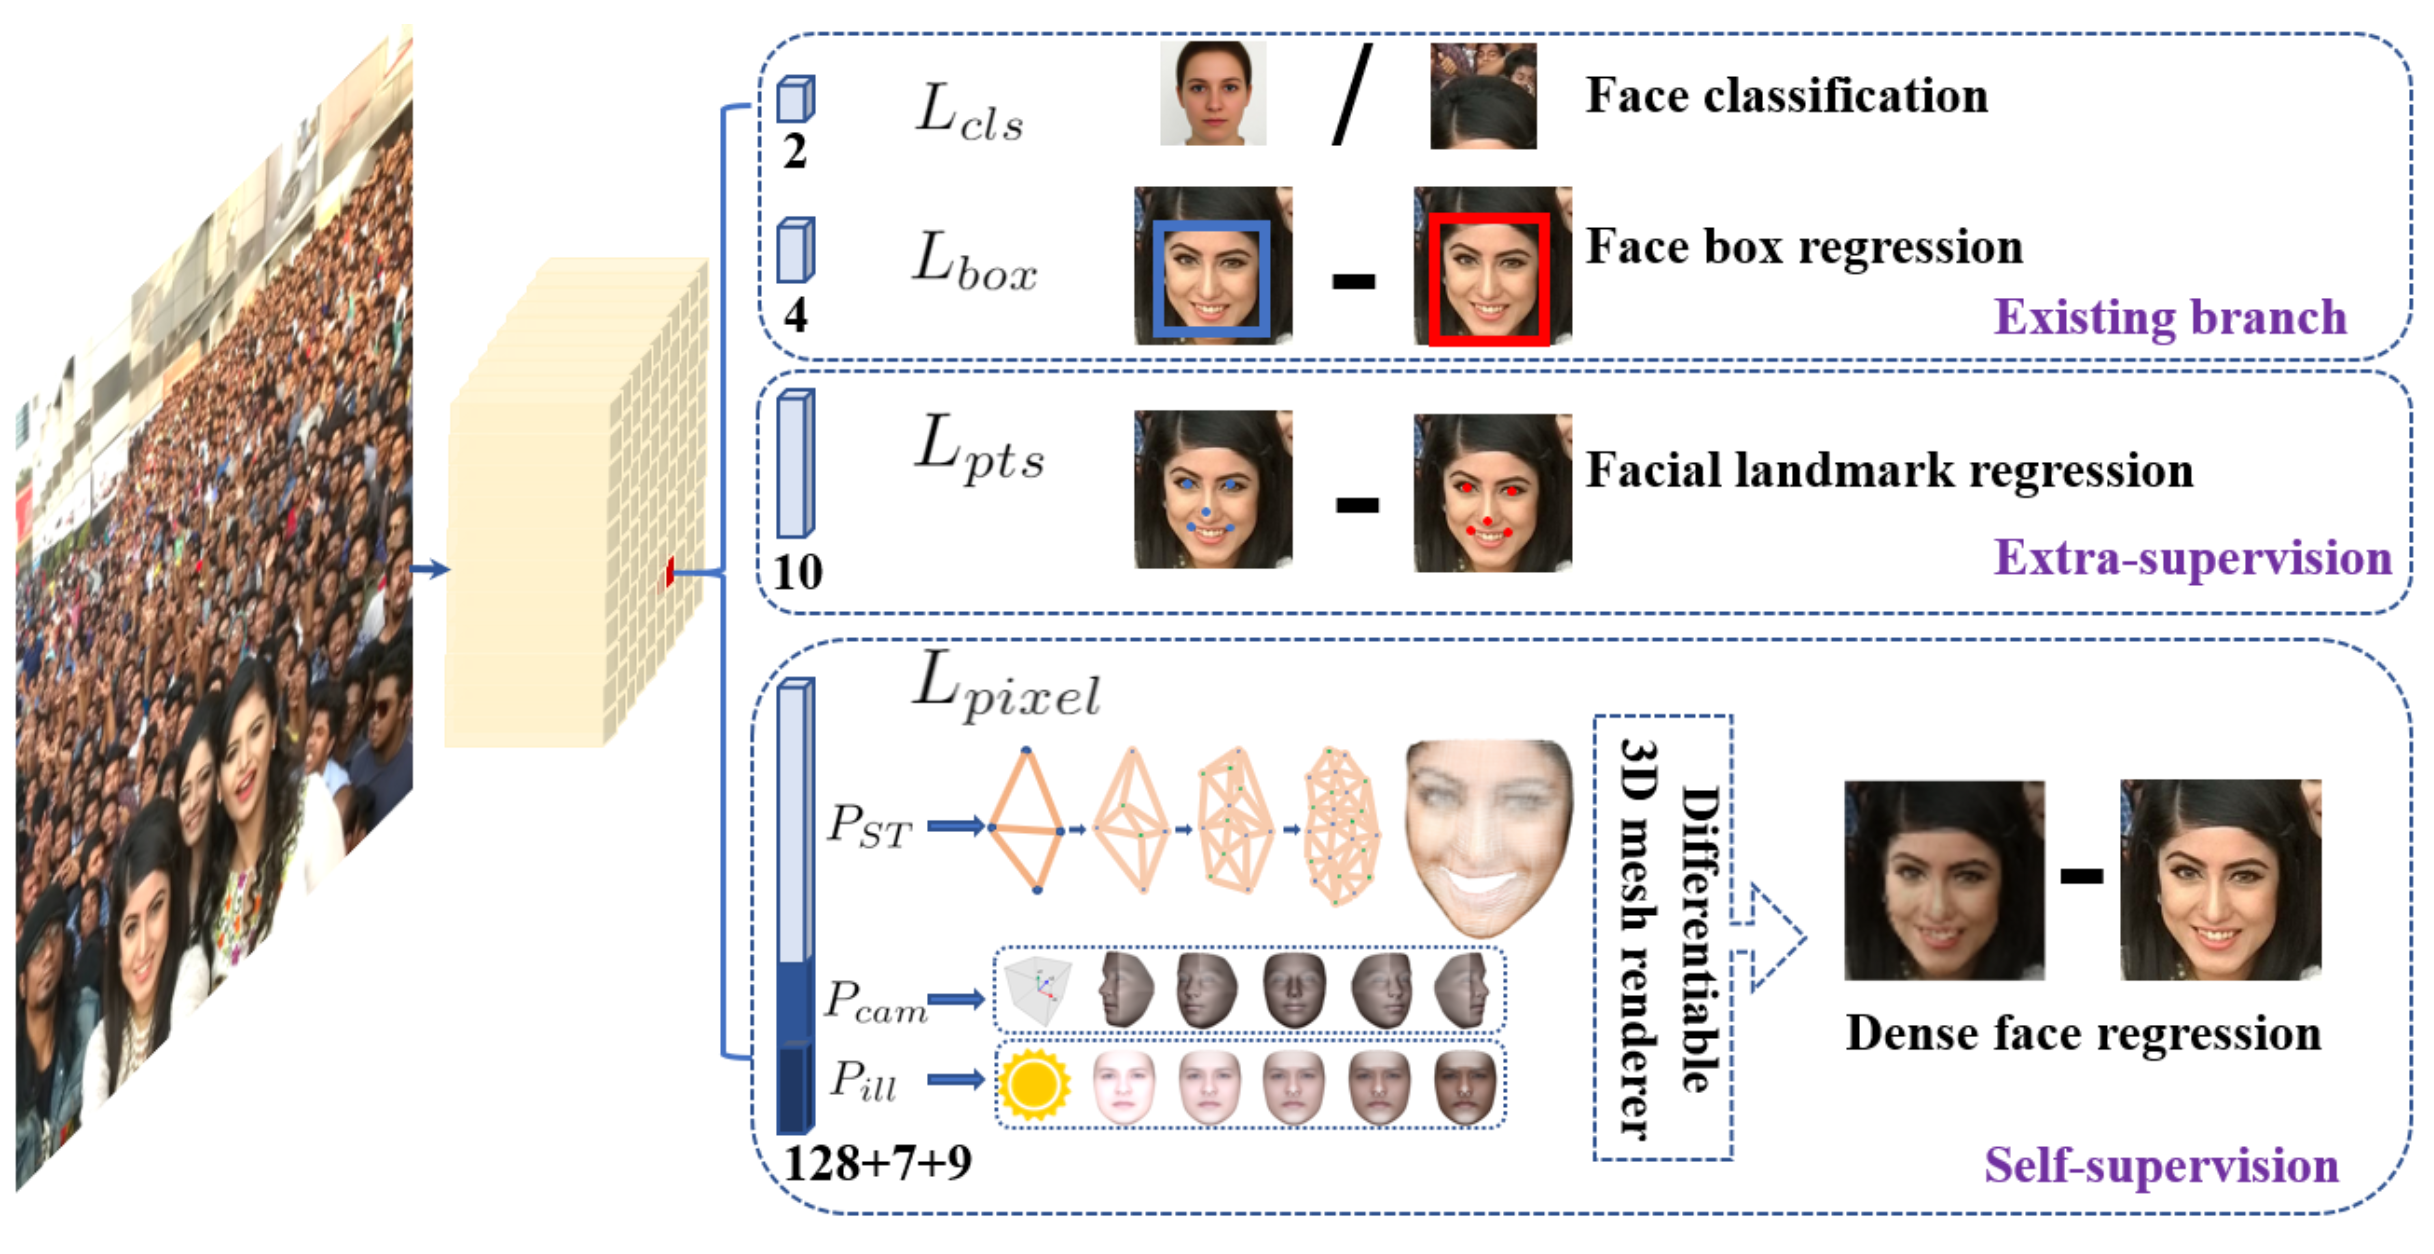
\includegraphics[width=10cm] {images/retinaface_loss_funcs}
        \caption{Ý tưởng hàm loss multi-task của mô hình RetinaFace. (Nguồn: \cite{deng2020retinaface})}
        \label{fig:retinaface_loss_funcs}
    \end{figure}

    Cụ thể hơn, trong quá trình train mô hình, với mỗi anchor, mô hình RetinaFace tối ưu hàm loss multi-task dưới đây:

    \begin{equation}
        \begin{split}
        L  & =  L_{cls}(p_i, p^{*}_i) + \lambda_1 p^{*}_i L_{box}(t_i, t^{*}_i) + \lambda_2 p^{*}_i L_{pts} (l_i, l^{*}_i) + \lambda_3 p^{*}_i L_{pixel}.\\
        \end{split}
        \label{eq:retinaface_loss}
    \end{equation}

    \noindent
    trong đó: \\
    - Các trọng số $\lambda_1, \lambda_2, \lambda_3$ được nhóm tác giả cấu hình mặc định là 0.25, 0.1 và 0.01. \\
    - Hàm loss phân lớp mặt: \\
    $L_{cls}(p_i, p^{*}_i)$ với $p_i$ là xác suất mà mô hình dự đoán một anchor có chứa là khuôn mặt hay không.
    Ta có $p^{*}_i = 1$ nếu anchor đó chứa khuôn mặt còn $p^{*}_i = 0$ nếu anchor đó không chứa khuôn là mặt. \\
    - Hàm loss hồi quy định vị vị trí của bbox: \\
    $L_{box}(t_i, t^{*}_i)$ với $t_i=\{t_x, t_y, t_w, t_h\}_i$ và $t^{*}_i=\{t^{*}_x, t^{*}_y, t^{*}_w, t^{*}_h\}_i$ lần lượt là bộ bốn tham số đại diện cho toạ độ của anchor mà mô hình dự đoán là mặt và bbox ground-truth từ bộ dữ liệu.
    (x là toạ độ x của điểm góc trái trên, y là toạ độ y của điểm góc trái trên, w là chiều rộng của bbox và h là chiều cao của bbox). \\
    - Hàm loss hồi quy định vị vị trí của landmarks: \\
    $L_{pts} (l_i, l^{*}_i)$ với $l_i=\{l_{x_1}, l_{y_1}, \dots , l_{x_5}, l_{y_5}\}_i$ và $l^{*}_i=\{l^{*}_{x_1}, l^{*}_{y_1}, \dots , l^{*}_{x_5}, l^{*}_{y_5}\}_i$ lần lượt là bộ mười tham số đại diện cho toạ độ của năm landmarks mà mô hình dự đoán ứng với mỗi bounding box dự đoán và năm ground-truth landmarks của mỗi groundtruth bounding box từ bộ dữ liệu. \\
    - Hàm loss hồi quy từng pixel của khuôn mặt: $L_{pixel}$ giúp bổ sung thêm thông tin và giúp loại bớt các trường hợp dự đoán nhầm background là khuôn mặt của mô hình. \\
    Hàm loss $L_{pixel}$ của mô hình RetinaFace là một hàm loss self-supervised learning.
    Cụ thể, RetinaFace sử dụng nghiên cứu \cite{zhou2019dense} dựa trên Graph Convolution Network để biến đối khuôn mặt từ bounding box trên ảnh sang dạng 3D, sau đó sử dụng mô hình \cite{genova2018unsupervised} để biến đổi ngược từ khuôn mặt dạng 3D trở về dạng 2D như trên ảnh thông thường.

    \begin{equation}
        L_{pixel}  = \frac{1}{W*H} \sum_{i}^{W} \sum_{j}^{H}  \|\mathcal{R}(\mathcal{D}_{P_{ST}},P_{cam},P_{ill})_{i,j} - I_{i,j}^*\|_1,\\
        \label{fig:retinaface_loss_pixel}
    \end{equation}

    \noindent
    trong đó: \\
    - $\mathcal{D}_{P_{ST}}$ là khuôn mặt sau khi biến đổi từ bounding box sang dạng 3D theo nghiên cứu \cite{zhou2019dense}. \\
    - $\mathcal{R}$ là mô hình biến đổi từ khuôn mặt dạng 3D trở về dạng 2D như trên ảnh thông thường theo nghiên cứu \cite{genova2018unsupervised}. \\
    - $P_{cam}, P_{ill}$ là các tham số của mô hình \cite{genova2018unsupervised}. \\
    - $W$ và $H$ lần lượt là chiều rộng và chiều dài của bounding box $I^*$.

    \noindent
    \textbf{\textit{Kết quả của mô hình RetinaFace}} \\
    Nhóm tác giả thực hiện thí nghiệm đánh giá mức độ đóng góp của các kỹ thuật trong mô hình RetinaFace. \\
    - FPN+Context: mô hình RetinaFace chỉ sử dụng kiến trúc FPN kết hợp các khối Context Module \cite{najibi2017ssh} với lớp Conv truyền thống. \\
    - +DCN: mô hình RetinaFace chỉ sử dụng kiến trúc FPN kết hợp các khối Context Module \cite{najibi2017ssh} với deformable convolution network \cite{dai2017deformable}. \\
    - +$L_{pts}$: mô hình RetinaFace chỉ sử dụng kiến trúc FPN kết hợp các khối Context Module \cite{najibi2017ssh} với deformable convolution network \cite{dai2017deformable} bổ sung thêm hàm loss về năm điểm landmarks. \\
    - +$L_{pixel}$: mô hình RetinaFace chỉ sử dụng kiến trúc FPN kết hợp các khối Context Module \cite{najibi2017ssh} với deformable convolution network \cite{dai2017deformable} bổ sung thêm hàm loss về self-supervised learning. \\
    - +$L_{pts}$+$L_{pixel}$: mô hình RetinaFace chỉ sử dụng kiến trúc FPN kết hợp các khối Context Module \cite{najibi2017ssh} với deformable convolution network \cite{dai2017deformable} bổ sung thêm hàm loss về năm điểm landmarks và hàm loss về self-supervised learning. \\

    \begin{figure}[H]
        \centering
        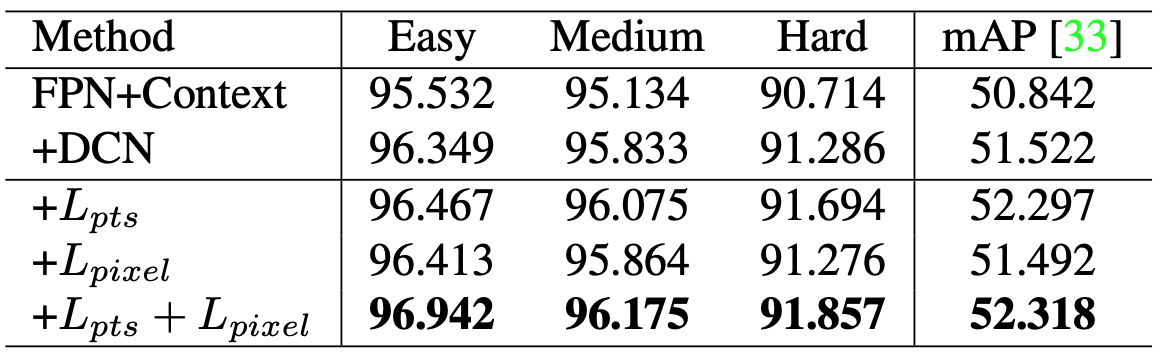
\includegraphics[width=10cm] {images/retinaface_results_1}
        \caption{So sánh kết quả việc sử dụng một số kỹ thuật trong mô hình RetinaFace. (Nguồn: \cite{deng2020retinaface})}
        \label{fig:retinaface_results_1}
    \end{figure}

    \noindent
    Cấu hình RetinaFace sử dụng tất cả các kỹ thuật trên cho kết quả tốt nhất trên cả ba bộ WIDER FACE val dễ, trung bình và khó.

    \noindent
    Việc mô hình RetinaFace cho kết quả tốt trên bài toán face detection giúp cải thiện kết quả của mô hình ArcFace trên bài toán face recognition trên các bộ dữ liệu khác nhau. \\
    - MTCNN+ArcFace: là cấu hình sử dụng mô hình MTCNN \cite{zhang2016joint} cho bài toán face detection và mô hình ArcFace \cite{deng2019arcface} cho bài toán face recognition. \\
    - RetinaFace+ArcFace: là cấu hình sử dụng mô hình RetinaFace cho bài toán face detection và mô hình ArcFace \cite{deng2019arcface} cho bài toán face recognition.

    \begin{figure}[H]
        \centering
        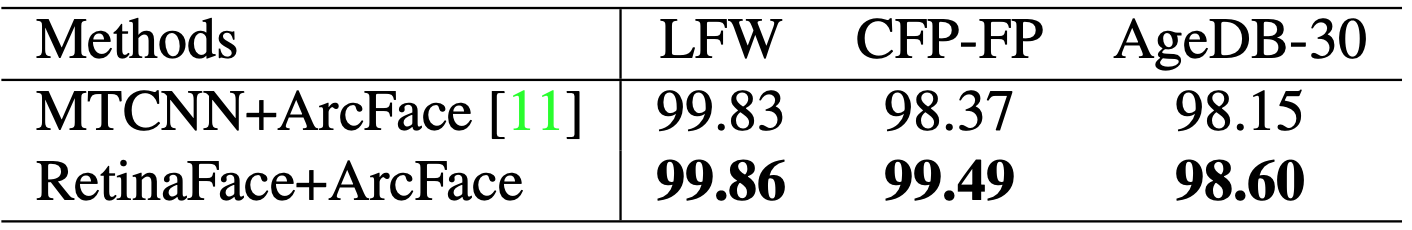
\includegraphics[width=10cm] {images/retinaface_results_2}
        \caption{Kết quả tốt của mô hình RetinaFace trên bài toán face detection giúp cải thiện kết quả trên cả bài toán face recognition. (Nguồn: \cite{deng2020retinaface})}
        \label{fig:retinaface_results_2}
    \end{figure}

    \noindent
    Ở thời điểm ra mắt, mô hình RetinaFace cho kết quả tốt nhất trên tất cả các bộ dữ liệu con của bộ WIDER FACE, bao gồm: \\
    - Với bộ val dễ đạt: 96.9\% \\
    - Với bộ val trung bình đạt: 96.1\% \\
    - Với bộ val khó đạt: 91.8\% \\
    - Với bộ test dễ đạt: 96.3\% \\
    - Với bộ test trung bình đạt: 95.6\% \\
    - Với bộ test khó đạt: 91.4\%

    \begin{figure}[H]
        \centering
        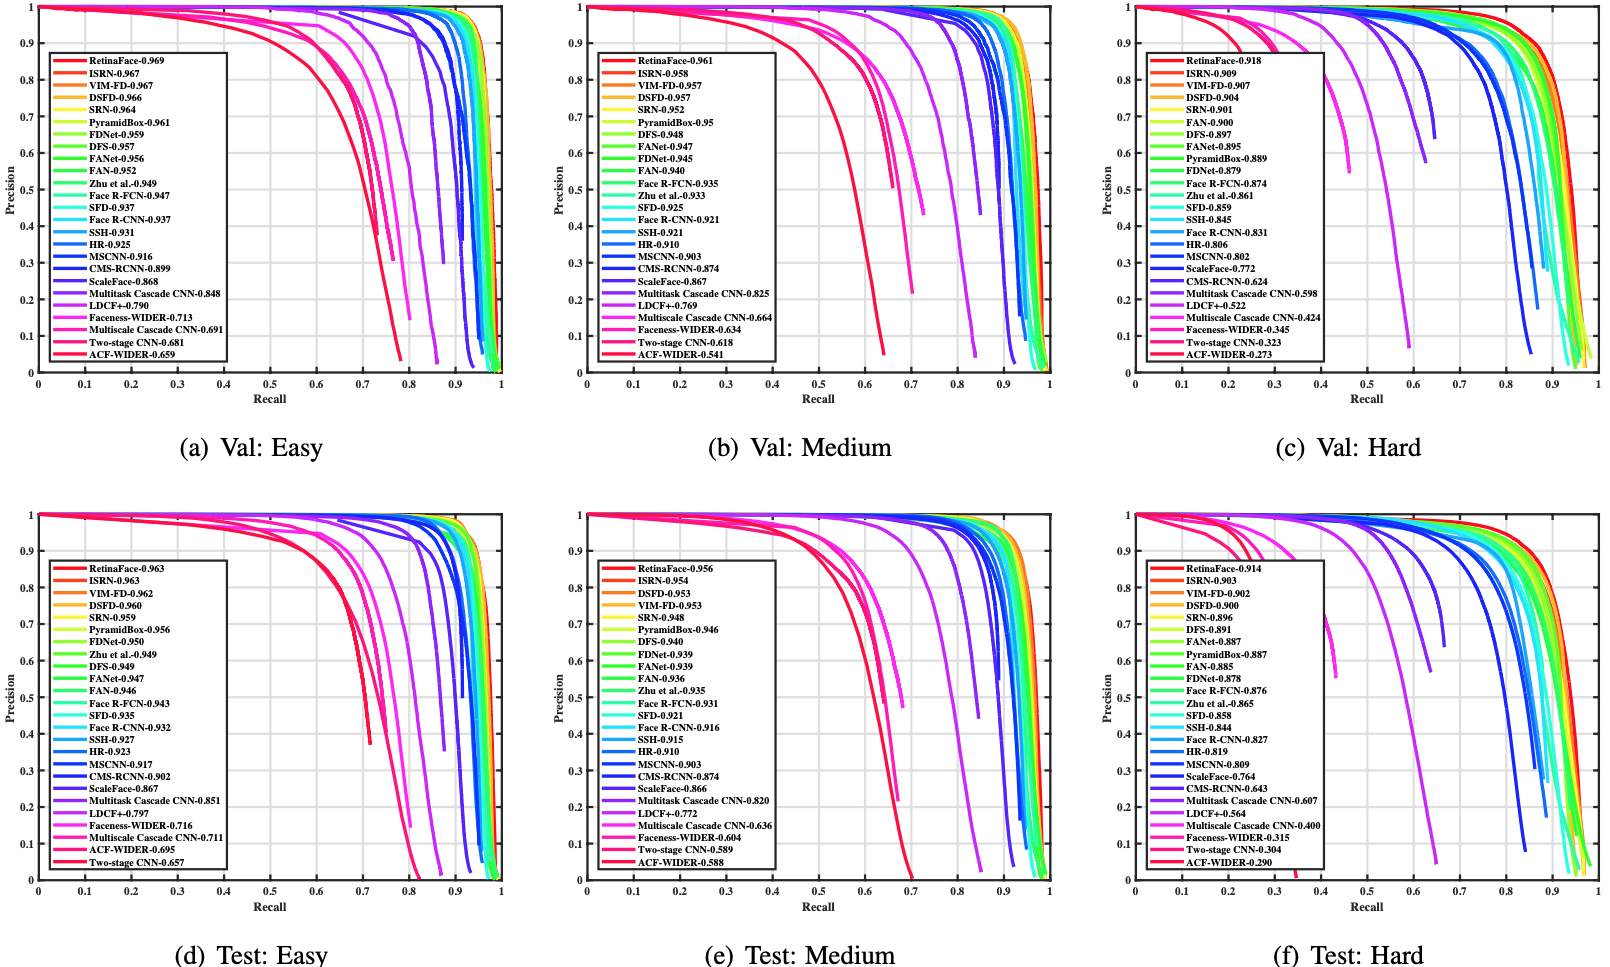
\includegraphics[width=10cm] {images/retinaface_results_3}
        \caption{Kết quả của về Precision - Recall của mô hình RetinaFace trên các bộ dữ liệu con của WIDER FACE. (Nguồn: \cite{deng2020retinaface})}
        \label{fig:retinaface_results_3}
    \end{figure}

    \noindent
    \textbf{\textit{Vấn đề tồn đọng của mô hình RetinaFace}} \\
    Mô hình RetinaFace đã giải quyết bài toán face detection với bộ dữ liệu WIDER FACE rất tốt, đạt độ chính xác cao.
    Tuy nhiên, khi xử lý với ảnh có kích thước lớn, mô hình RetinaFace muốn giữ được kết quả tốt cần mất thời gian chạy khá lâu.
    Điều này khiến cho mô hình RetinaFace thường chỉ nằm ở mức độ nghiên cứu và khó có thể được sử dụng trong các ứng dụng thực tế.
}
    \retinaface
}
    \theory
    
    \newpage
    \def\proposedmodel{
    \section{Mô hình đề xuất}

    \subsection{Tổng quan ý tưởng của mô hình RetinaFocus}
    \def\retinafocusidea{
    Lấy cảm hứng từ hai mô hình RetinaFace \cite{deng2020retinaface} và AutoFocus \index{AutoFocus} \cite{najibi2019autofocus}, mô hình RetinaFocus được xây dựng nhằm tận dụng điểm mạnh và khắc phục điểm yếu của cả hai mô hình trên trong một mô hình duy nhất, từ đó, giải quyết tốt bài toán nhận diện khuôn mặt trong ảnh chất lượng cao.

    \noindent
    Mô hình RetinaFace là một mô hình có đạt độ chính xác tương đối cao trên bộ dữ liệu WIDER FACE cùng với tốc độ xử lý đạt mức chấp nhận được.
    Mặc dù sử dụng FPN trong kiến trúc backbone của mình, mô hình RetinaFace vẫn chưa thể dự đoán với vị trí bbox chính xác và với độ tự tin cao hết những mặt có kích thước nhỏ.
    Do đó, khi xử lý ảnh có kích thước lớn, để duy trì được độ chính xác cao, nhóm tác giả vẫn sử dụng chiến lược Image Pyramids và điều đó khiến cho tốc độ xử lý của RetinaFace tăng lên nhiều lần. \\
    Bên cạnh đó, mô hình AutoFocus \index{AutoFocus}, lại là một giải pháp rất thông minh để xử lý ảnh với chiến lược Image Pyramids nhưng với tốc độ cao và chi phí tính toán thấp. \\
    Từ những điểm yếu của mô hình RetinaFace khi xử lý ảnh chất lượng cao và những điểm mạnh của mô hình AutoFocus \index{AutoFocus}, chúng tôi đề xuất mô hình RetinaFocus giải bài toán nhận diện khuôn mặt trong ảnh chất lượng cao với độ chính xác tương đương và cải thiện đáng kể tốc độ tính toán.

    \noindent
    \textbf{\textit{Kiến trúc mô hình RetinaFocus}} \\
    Kiến trúc mô hình RetinaFocus lấy mô hình RetinaFace làm nền tảng, kết hợp cùng Nhánh Focus \index{nhánh Focus} của mô hình AutoFocus \index{AutoFocus}.
    Nói cách khác, mô hình RetinaFace được sử dụng để thay thế cho mô hình Faster R-CNN của Nhánh Detection \index{nhánh Detection} trong mô hình AutoFocus \index{AutoFocus}.
    Cụ thể hơn, một trong số các feature maps \index{feature maps} được trích xuất từ backbone FPN, bên cạnh việc được qua các Context Module như trong mô hình RetinaFace nguyên bản, còn được đưa qua các lớp Conv \index{lớp Conv} của Nhánh Focus \index{nhánh Focus} giúp xác định được khu vực đáng chú ý trên ảnh và loại bỏ các khu vực khả năng cao không chứa khuôn mặt.

    \begin{figure}[H]
        \centering
        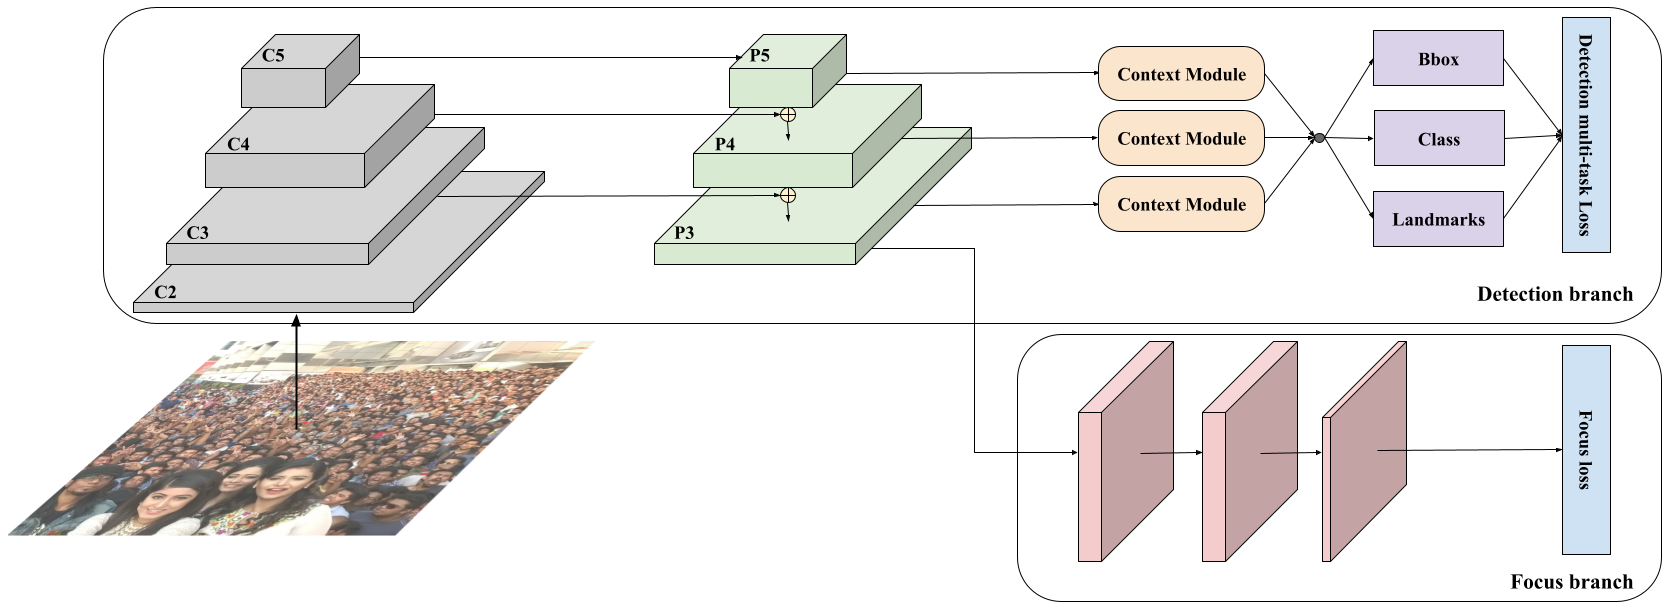
\includegraphics[width=13cm] {images/retinafocus_architecture}
        \caption{Kiến trúc của mô hình RetinaFocus.}
        \label{fig:retinafocus_architecture}
    \end{figure}

    \noindent
    Hình trên là một ví dụ về kiến trúc mô hình RetinaFocus khi sử dụng feature maps \index{feature maps} P3 của FPN làm đầu vào cho Nhánh Focus \index{nhánh Focus}.
    Các feature maps \index{feature maps} khác của FPN cũng đều có thể được sử dụng làm đầu vào cho Nhánh Focus \index{nhánh Focus} và kết quả so sánh độ hiệu quả của các feature maps \index{feature maps} này sẽ được bàn luận kỹ hơn ở phần dưới. \\
    Đối với Nhánh Detection \index{nhánh Detection} của RetinaFocus, đầu ra được giữ nguyên so với mô hình RetinaFace nguyên bản gồm toạ độ của bounding box \index{bounding box} dự đoán của mô hình, toạ độ của landmarks của khuôn mặt và xác suất mà bounding box \index{bounding box} dự đoán đó chứa khuôn mặt.
    Các đầu ra này của Nhánh Detection \index{nhánh Detection}, sau đó, tiếp tục được đưa vào hàm loss multi-task, tương tự như mô hình RetinaFace. \\
    Đối với Nhánh Focus \index{nhánh Focus} của RetinaFocus, đầu ra vẫn là mask mà mô hình dự đoán và được đưa vào hàm loss để so sánh với mask gồm các giá trị -1, 0, 1 được sinh ra từ thuật toán Focus Pixel  của mô hình AutoFocus \index{AutoFocus}.

    \noindent
    \textbf{\textit{Chuẩn bị dữ liệu cho Nhánh Focus của mô hình}} \index{nhánh Focus} \\
    Để sử dụng mô hình AutoFocus \index{AutoFocus} một cách hiệu quả, ta cần xây dựng được bộ tham số yêu cầu cho Thuật toán Focus Pixel, cụ thể là ba tham số $a, b, c$, đặc biệt là hai tham số $a$ và $b$ giúp định nghĩa ra khoảng kích thước bounding box \index{bounding box} cần được focus.
    Để xây dựng được bộ tham số này, ta cần phân tích điểm yếu của Nhánh Detection \index{nhánh Detection} (cụ thể chính là mô hình RetinaFace) trên bộ dữ liệu WIDER FACE.
    Từ những điểm yếu, ta lựa chọn bộ tham số của Nhánh Focus \index{nhánh Focus} nhằm giúp cho Nhánh Focus \index{nhánh Focus} xác định được những vùng mà Nhánh Detection \index{nhánh Detection} dự đoán yếu và zoom vào giúp Nhánh Detection \index{nhánh Detection} dự đoán chính xác hơn.

    \begin{figure}[H]
        \centering
        \subfigure[]{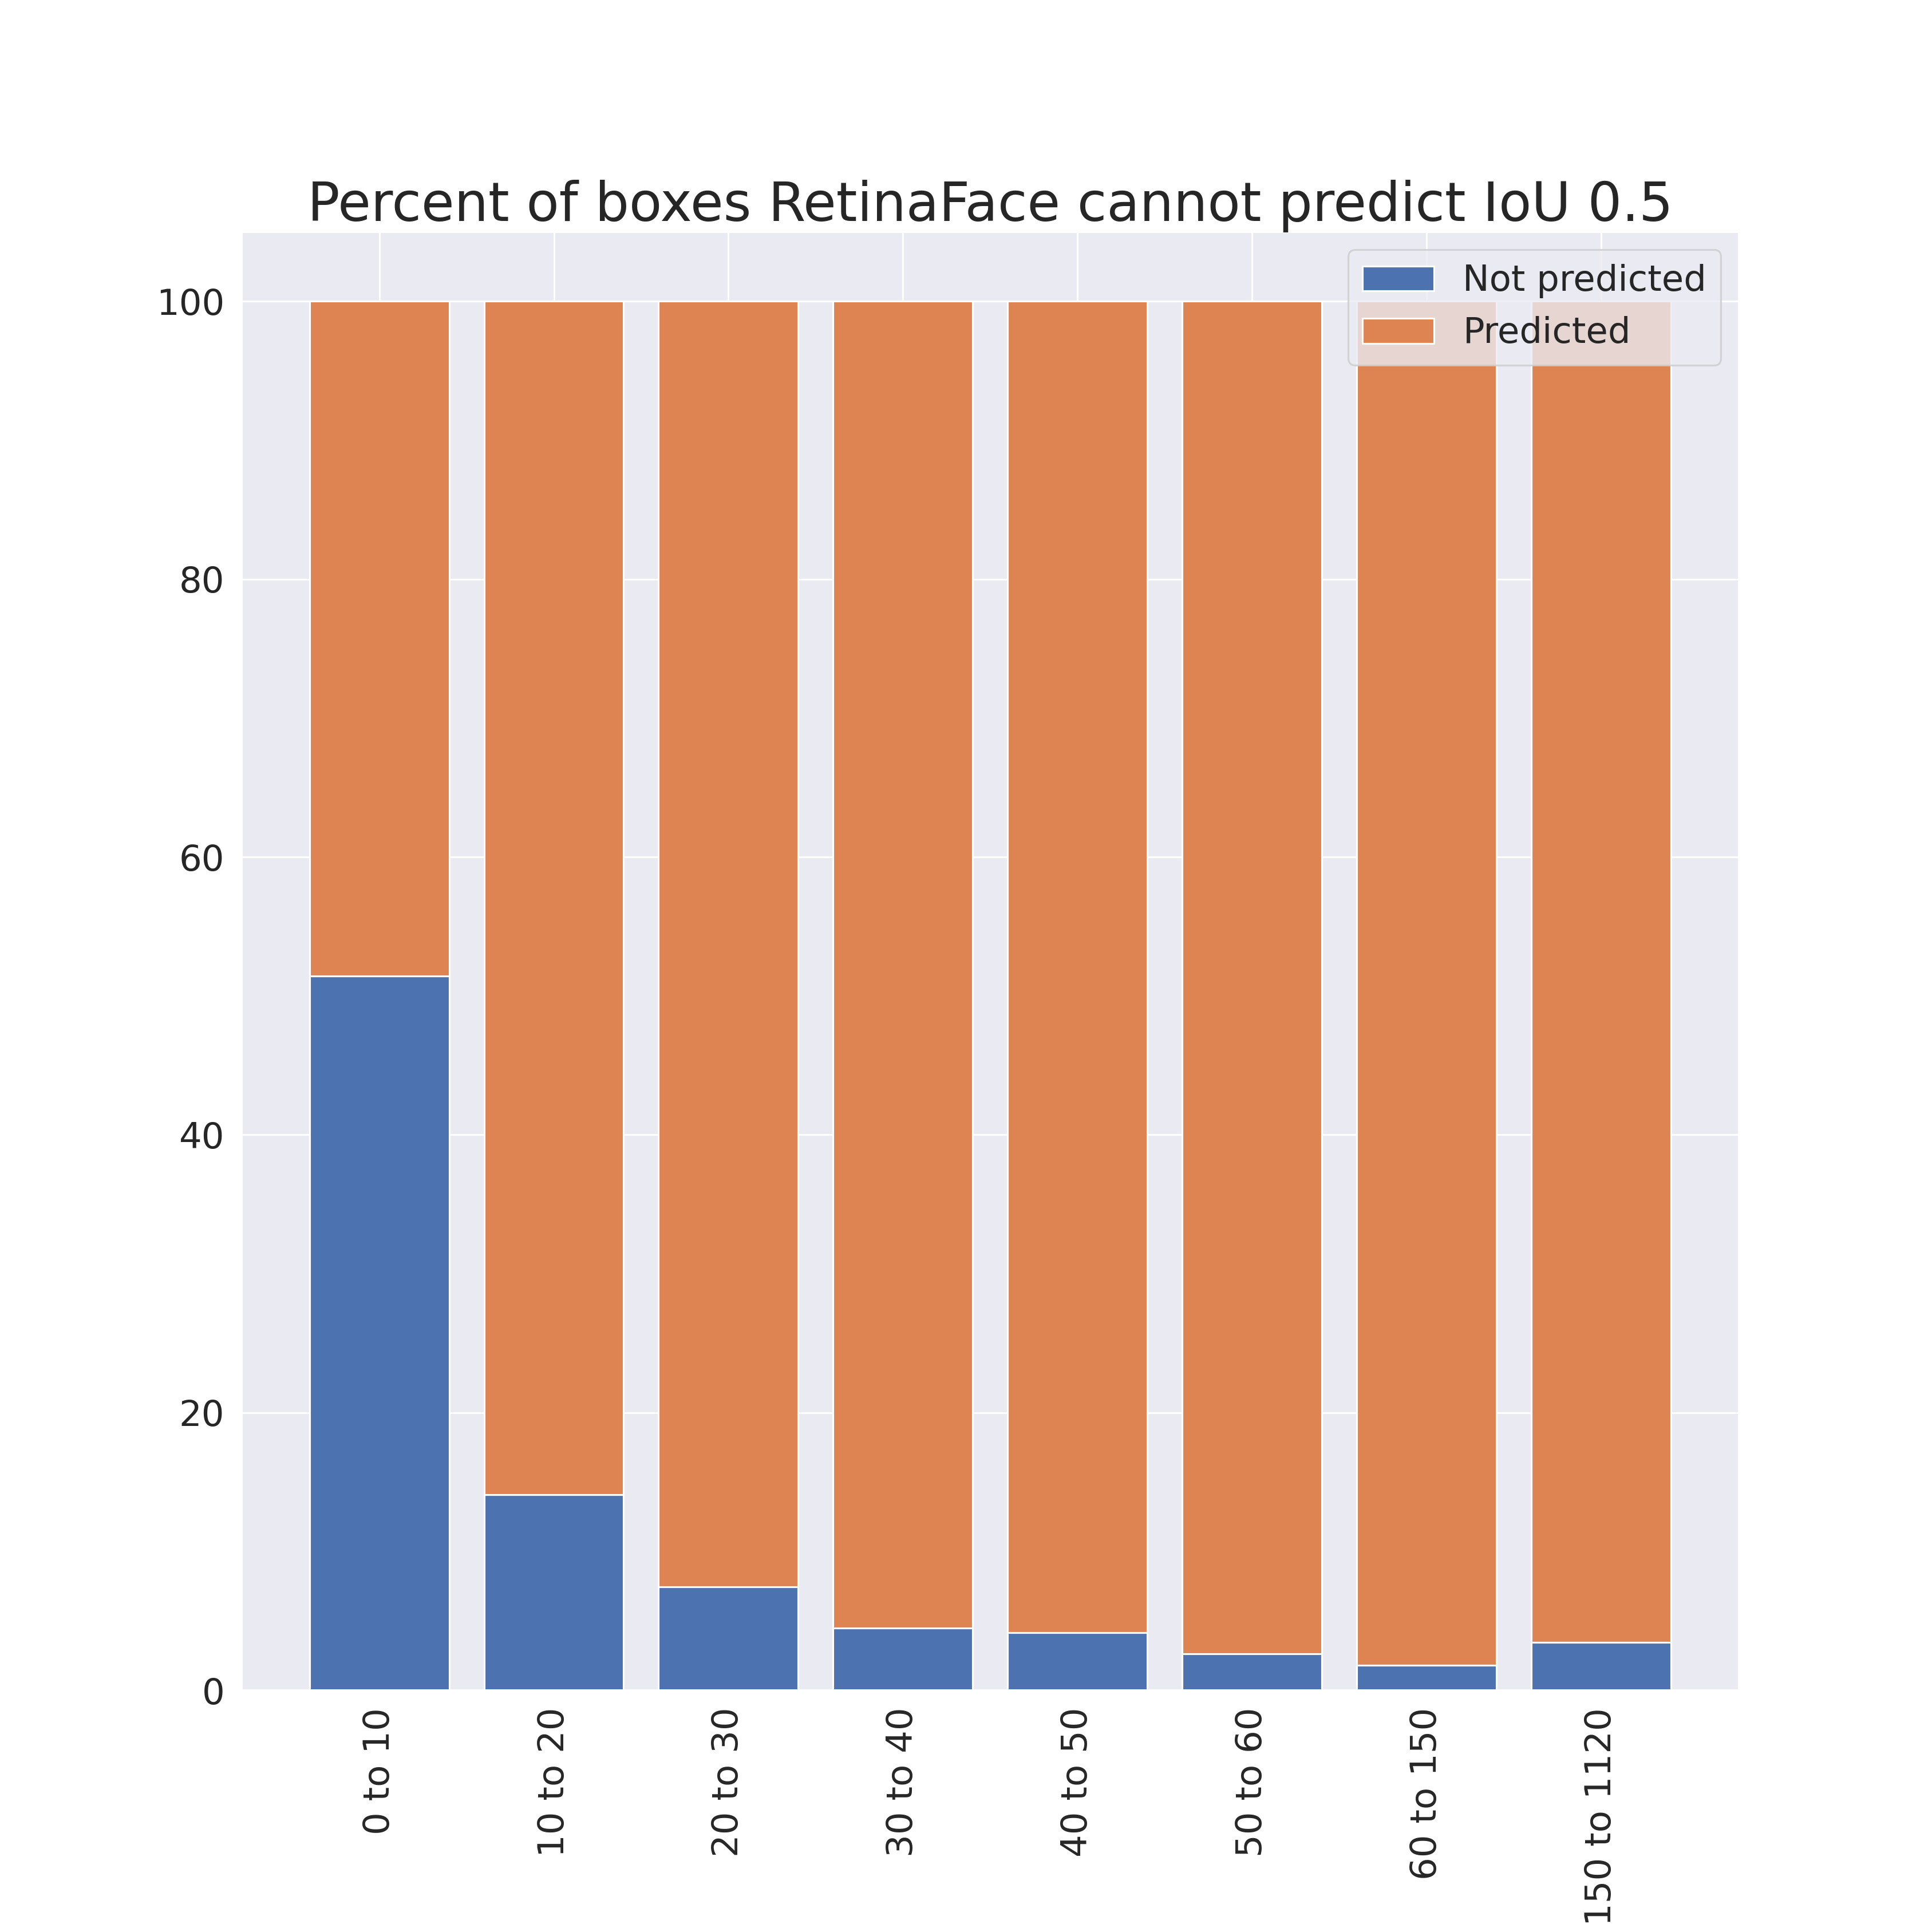
\includegraphics[width=0.32\textwidth, trim={2.3cm 2.3cm 2.3cm 2.3cm}, clip]{images/retinafocus_iou_50_compare_percent}} 
        \subfigure[]{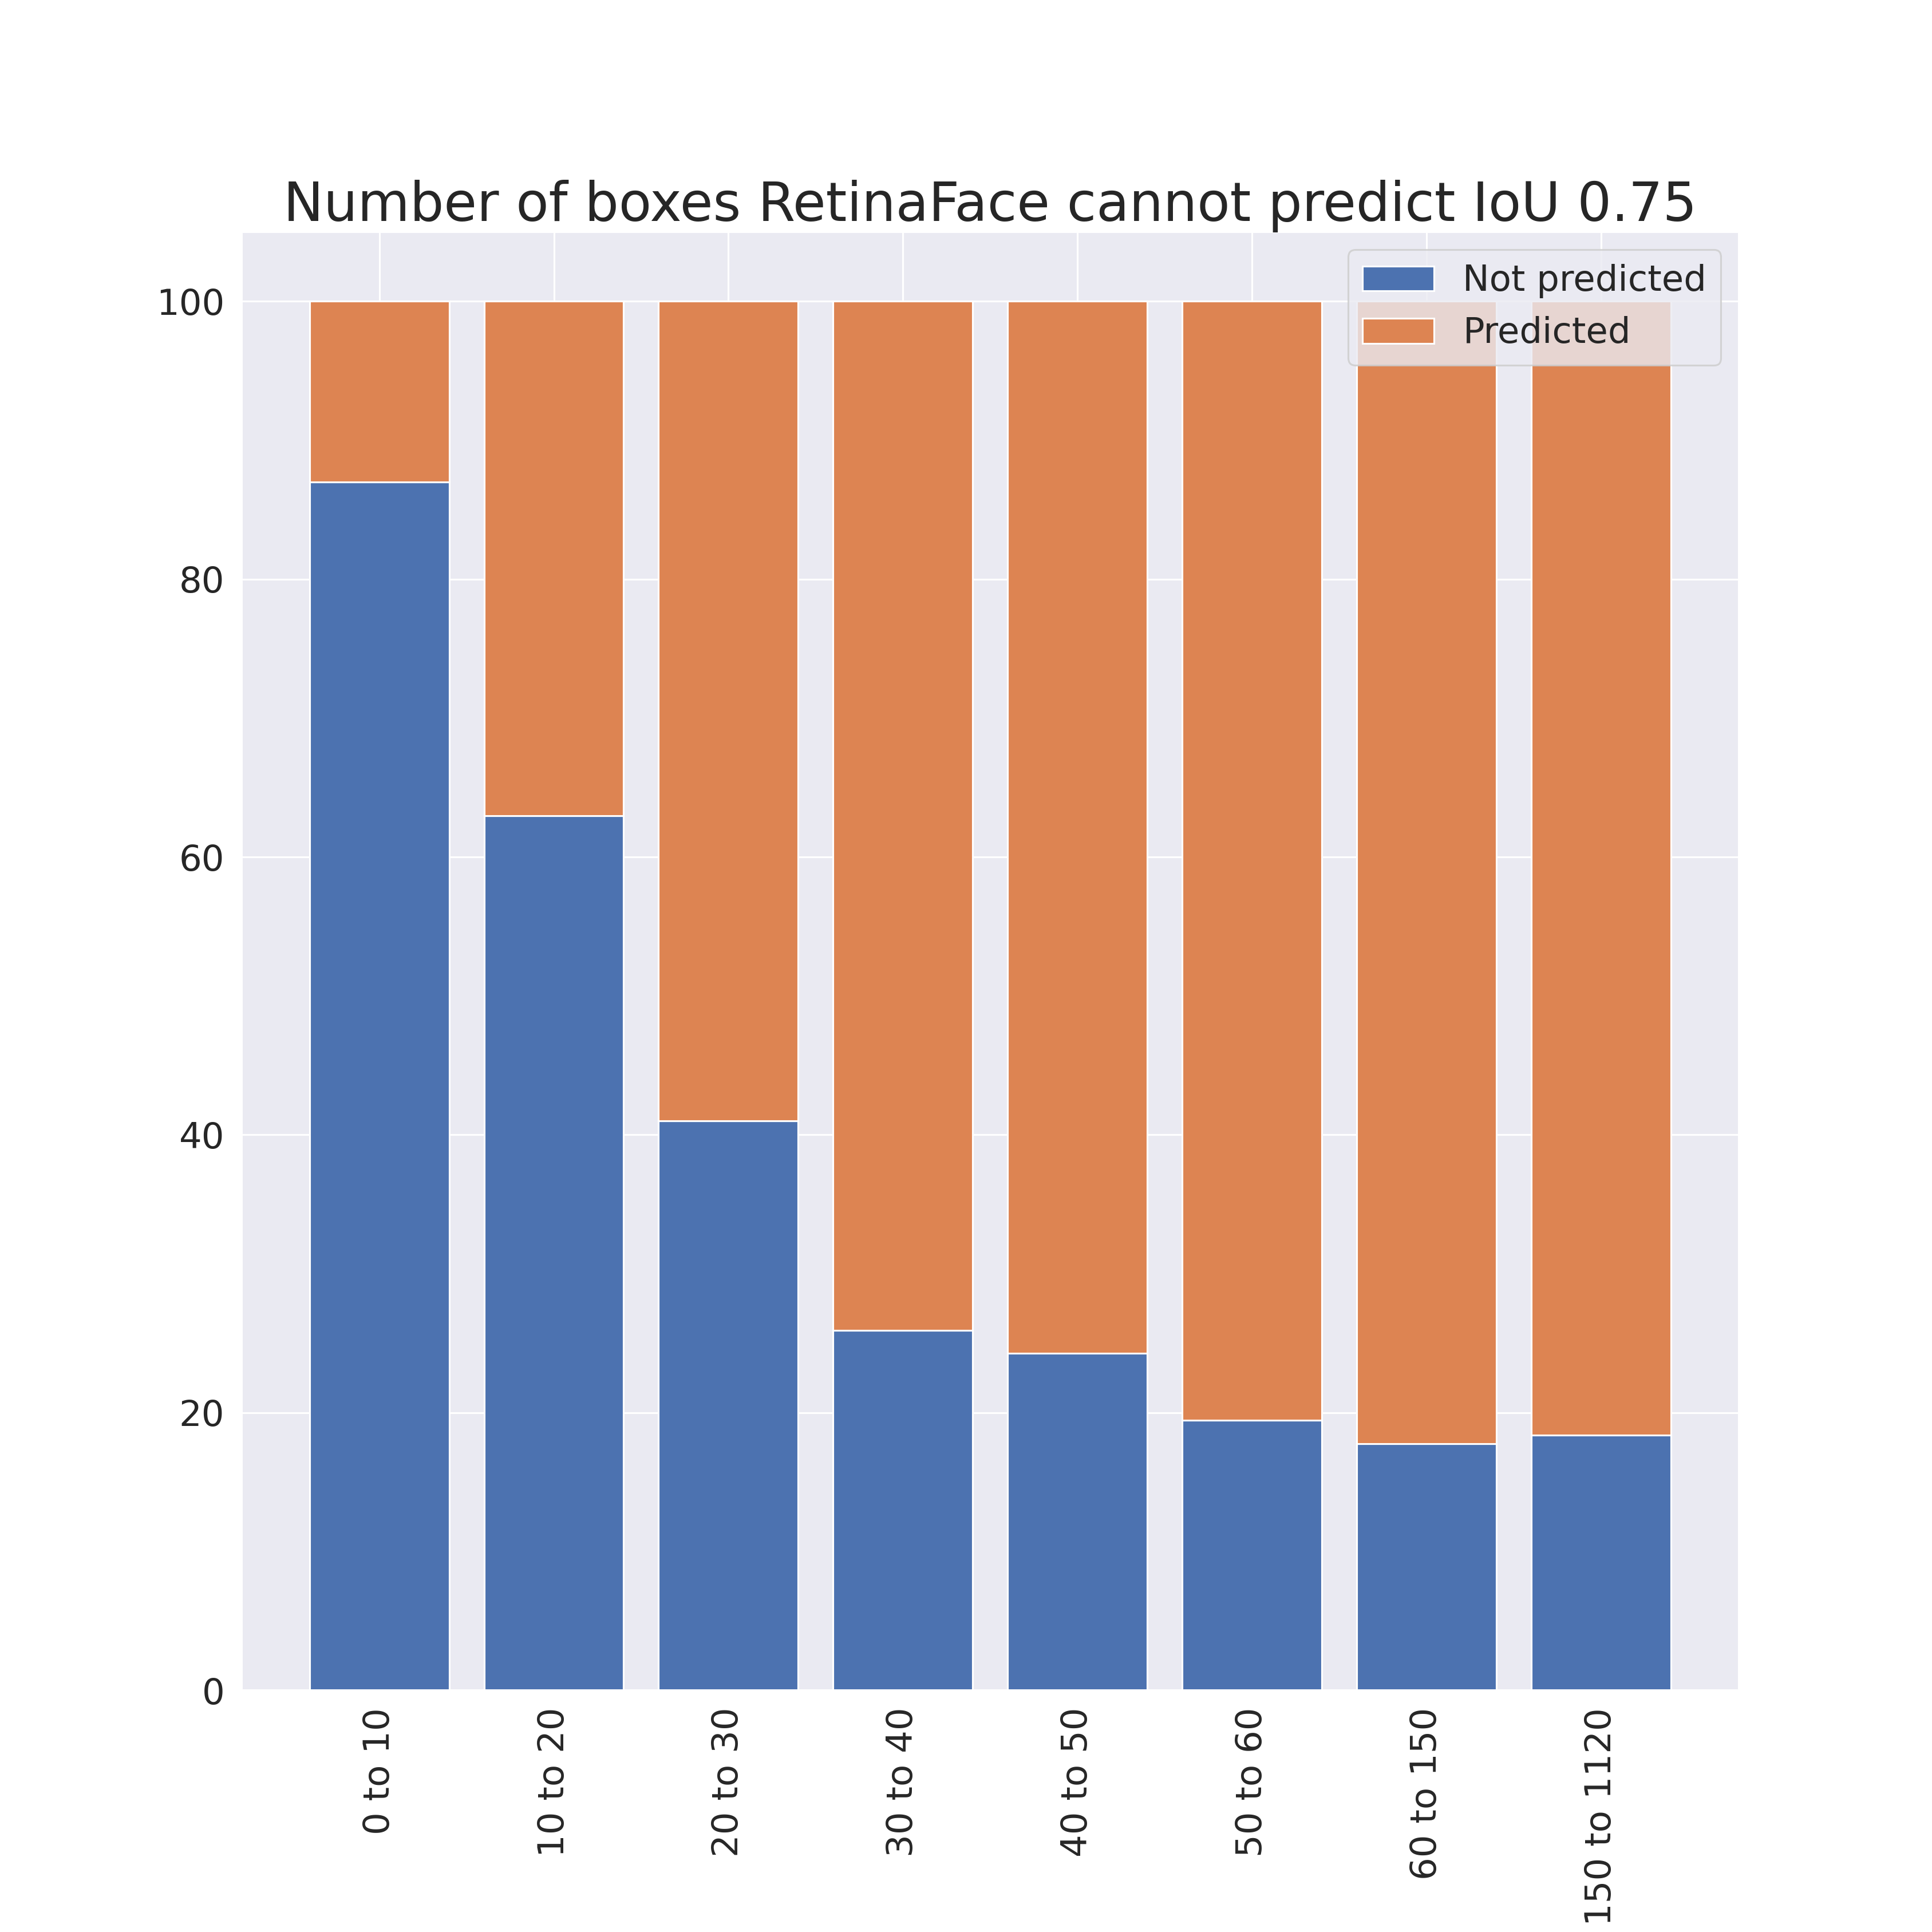
\includegraphics[width=0.32\textwidth, trim={2.3cm 2.3cm 2.3cm 2.3cm}, clip]{images/retinafocus_iou_75_compare_percent}} 
        \subfigure[]{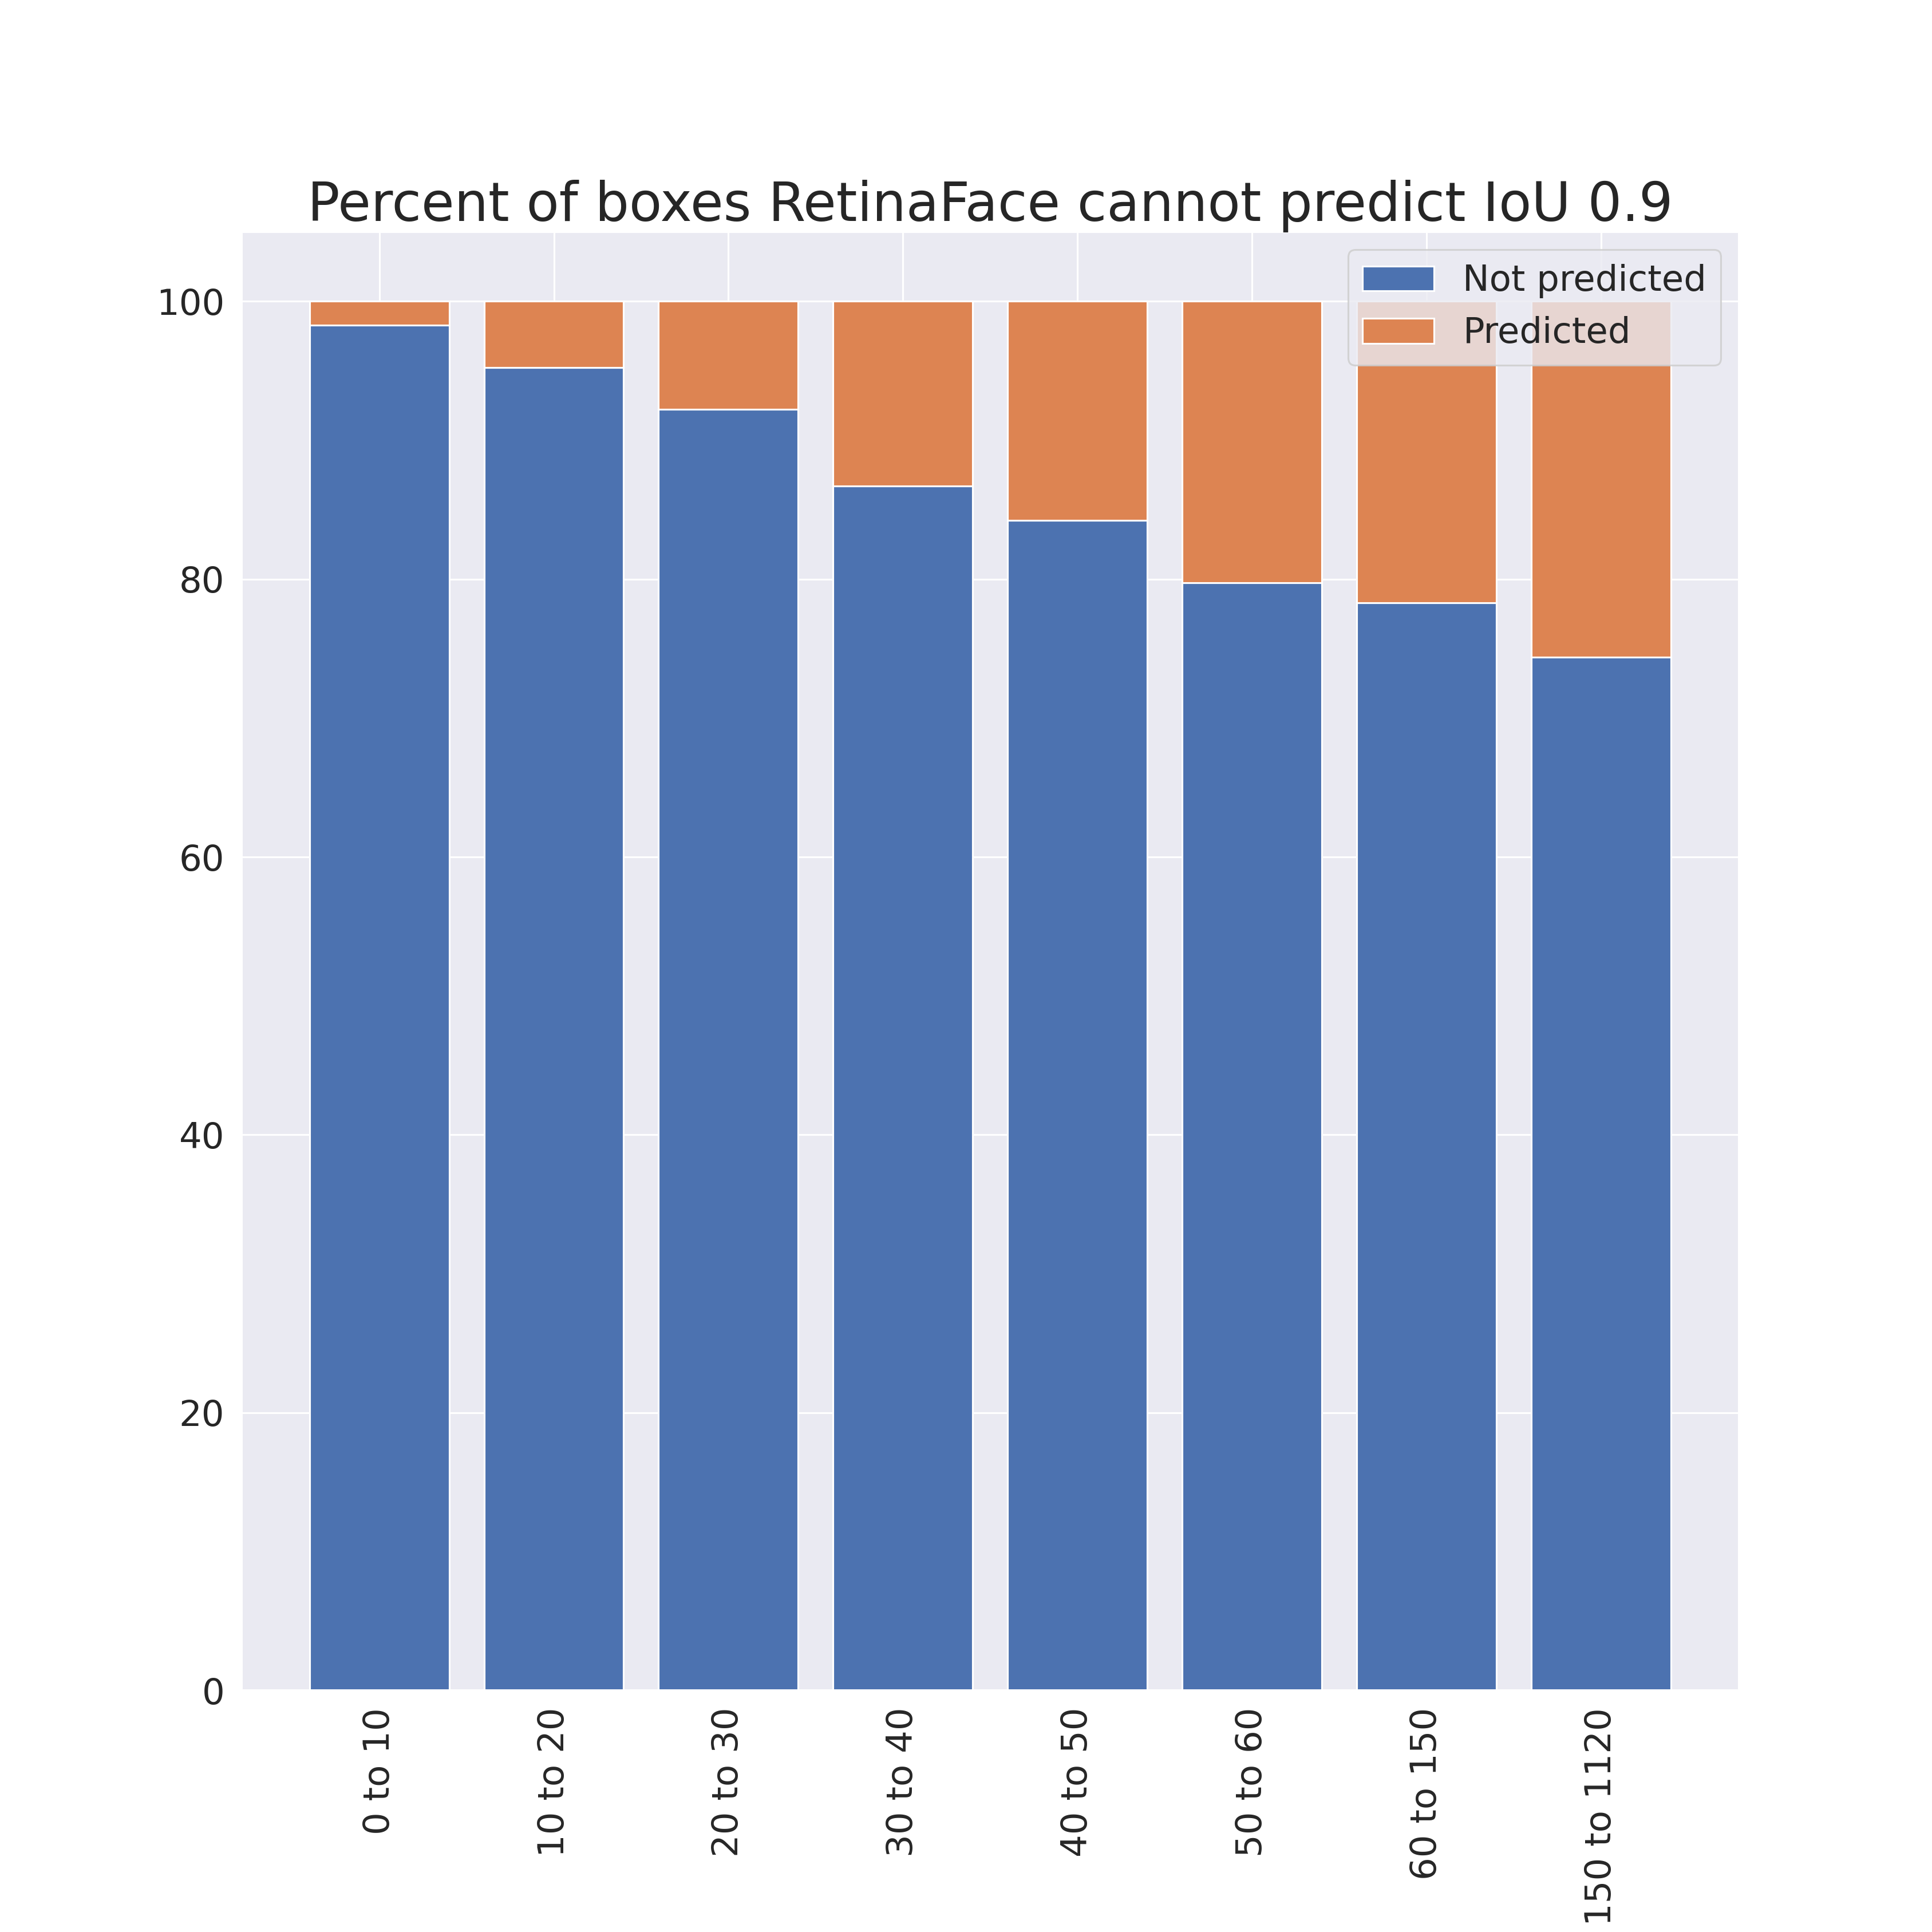
\includegraphics[width=0.32\textwidth, trim={2.3cm 2.3cm 2.3cm 2.3cm}, clip]{images/retinafocus_iou_90_compare_percent}} 
        \caption{Tỷ lệ số lượng bounding box \index{bounding box} mà mô hình RetinaFace dự đoán ra và không dự đoán ra tương ứng với IoU \index{IoU} 0.5 (a), IoU \index{IoU} 0.75 (b), IoU \index{IoU} 0.9 (c)}
        \label{fig:retinafocus_iou_compare_percent}
    \end{figure}

    \noindent
    Trong hình \ref{fig:retinafocus_iou_compare_percent}, trên cả ba mức IoU \index{IoU}, tỷ lệ số lượng bounding box \index{bounding box} mà mô hình RetinaFace không dự đoán ra đối với nhóm các bounding box \index{bounding box} nhỏ từ 0 pixels \index{pixels} đến 30 pixels \index{pixels} và đặc biệt là từ 0 pixels \index{pixels} đến 10 pixels \index{pixels} đều cao vượt trội so với các kích thước bounding box \index{bounding box} khác.

    \begin{figure}[H]
        \centering
        \subfigure[]{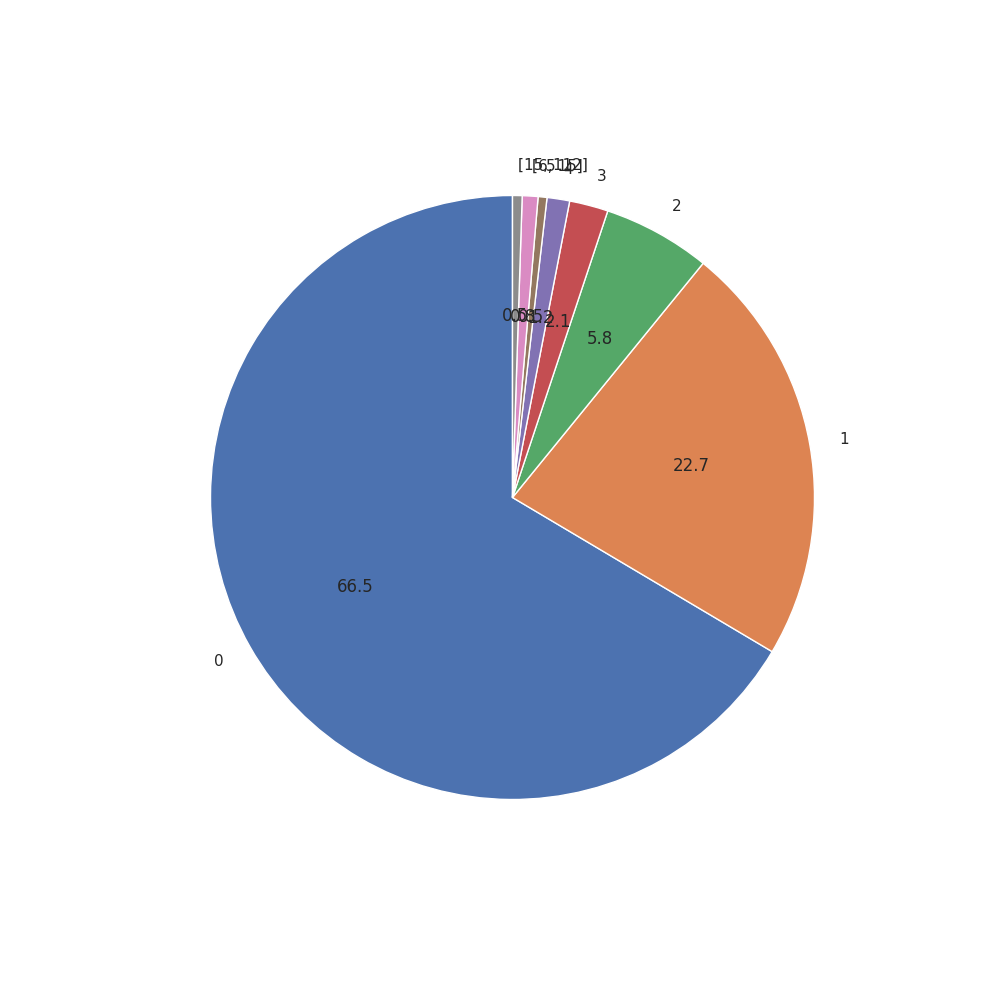
\includegraphics[width=0.32\textwidth, trim={5cm 4.7cm 4.3cm 4.6cm}, clip]{images/retinafocus_iou_50_lower}} 
        \subfigure[]{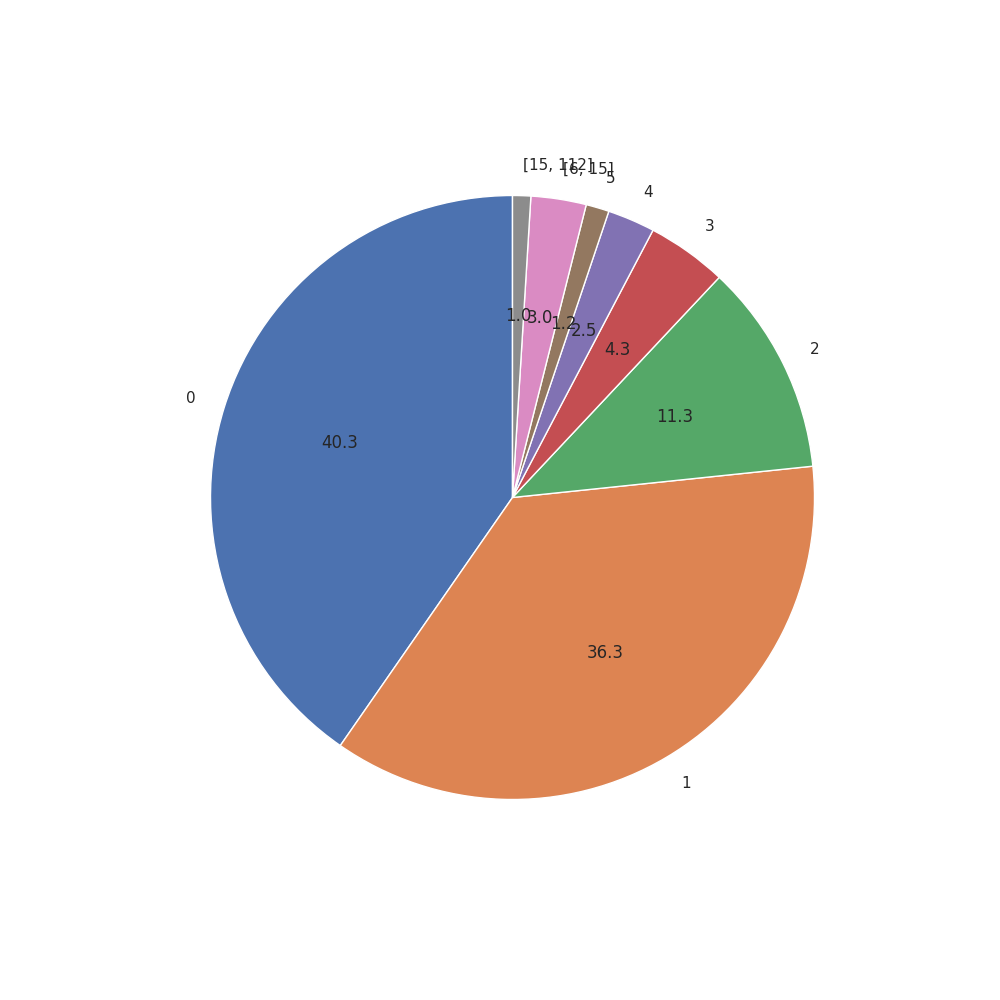
\includegraphics[width=0.32\textwidth, trim={5cm 4.7cm 4.3cm 4.6cm}, clip]{images/retinafocus_iou_75_lower}} 
        \subfigure[]{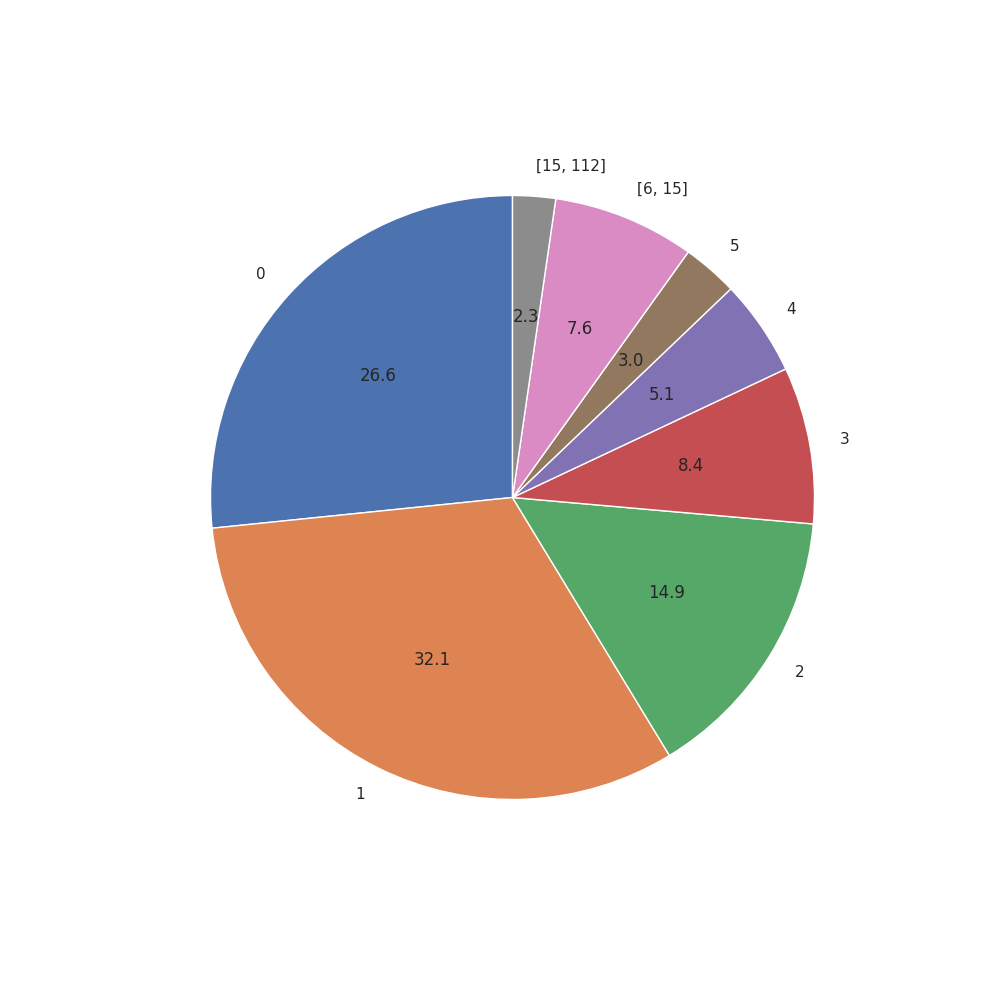
\includegraphics[width=0.32\textwidth, trim={5cm 4.7cm 4.3cm 4.6cm}, clip]{images/retinafocus_iou_90_lower}} 
        \caption{Tỷ lệ các kích thước của bounding box \index{bounding box} mà RetinaFace không dự đoán ra tương ứng với IoU \index{IoU} 0.5 (a), IoU \index{IoU} 0.75 (b), IoU \index{IoU} 0.9 (c)}
        \label{fig:retinafocus_iou_lower}
    \end{figure}

    \noindent
    Cụ thể hơn, trong hình \ref{fig:retinafocus_iou_lower}, dù xét ở mức IoU \index{IoU} nào, thì các bounding box \index{bounding box} có kích thước nhỏ từ 0 đến 60 đều chiếm tổng tỷ lệ lớn, cụ thể ... đối với IoU \index{IoU} 0.5, ... đối với IoU \index{IoU} 0.75 và ... đối với IoU \index{IoU} 0.9.

    \noindent
    Hơn nữa, với kiến trúc của FPN như hình \ref{fig:retinafocus_architecture}, một bounding box \index{bounding box} có kích thước $4 \times 4$ ở ảnh đầu vào sẽ có tương ứng một khu vực có kích thước $2 \times 2$ ở feature maps \index{feature maps} ${C}_{2}$ và ${P}_{2}$, $1 \times 1$ ở feature maps \index{feature maps} ${C}_{3}$ và ${P}_{3}$ và gần như không còn thông tin ở các feature maps \index{feature maps} từ ${C}_{4}$ và ${P}_{4}$ trở đi.
    Điều này khiến cho các bounding box \index{bounding box} này trở thành các điểm dữ liệu nhiễu của Nhánh Focus \index{nhánh Focus}, khiến cho việc học của Nhánh Focus \index{nhánh Focus} bị giảm hiệu quả.

    \noindent
    Từ những phân tích trên, chúng tôi lựa chọn lần lượt các tham số $a = 5, b = 60, c = 150$ tương ứng với groundtruth \index{groundtruth} bounding box \index{bounding box} có kích thước từ $5 \times 5$ đến $60 \times 60$ là các bounding box \index{bounding box} cần được focus, các groundtruth \index{groundtruth} bounding box \index{bounding box} có kích thước dưới $5 \times 5$ hoặc từ $60 \times 60$ đến $150 \times 150$ là các bounding box \index{bounding box} không cần quan tâm và các groundtruth \index{groundtruth} bounding box \index{bounding box} có kích thước trên $150 \times 150$ là các bounding box \index{bounding box} được coi như là background \index{background}.
}
    \retinafocusidea

    \subsection{Chi tiết kiến trúc của mô hình RetinaFocus}
    \def\retinafocusarchitecture{
    \subsubsection{Mô hình RetinaFace}
    \def\detectionbranch{
    Nhánh xác định đối tượng\index{nhánh xác định đối tượng} của RetinaFocus được xây dựng dựa trên mô hình RetinaFace \cite{deng2020retinaface}, một mô hình một pha\index{một pha} giải quyết bài toán nhận diện khuôn mặt và đạt kết quả tốt trên bộ dữ liệu WIDER FACE \cite{yang2016wider}. \\

    \noindent
    \textbf{\textit{Giới thiệu chung về mô hình RetinaFace nguyên bản}} \\
    Mô hình RetinaFace \cite{deng2020retinaface} nguyên bản đạt độ chính xác lần lượt là 96.9\%, 96.1\% và 91.8\% trên bộ dữ liệu WIDER FACE val easy, medium và hard.
    Trong khi đó, với bộ dữ liệu WIDER FACE test, Mô hình RetinaFace \cite{deng2020retinaface} nguyên bản đạt độ chính xác lần lượt là 96.3\%, 95.6\% và 91.4\% tương ứng với bộ easy, medium và hard.

    \begin{figure}[H]
        \centering
        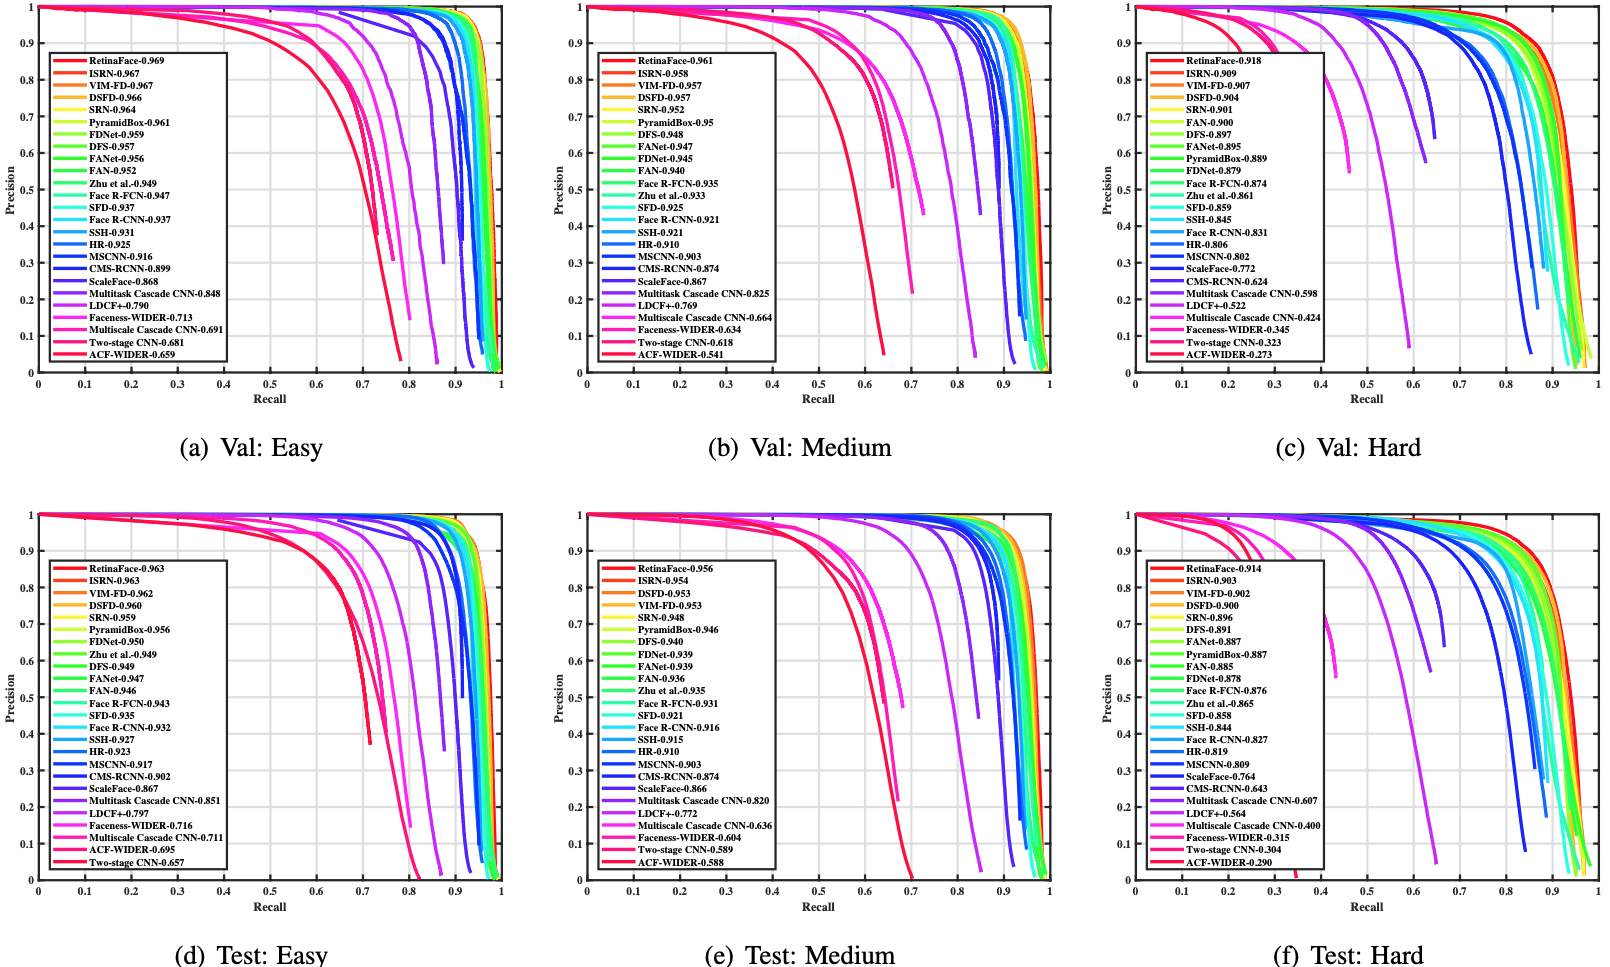
\includegraphics[width=15cm] {images/retinaface_results_3}
        \caption{Kết quả của mô hình RetinaFace nguyên bản trên bộ dữ liệu WIDER FACE val và test. (Nguồn: \cite{deng2020retinaface})}
        \label{fig:retinaface_results_3}
    \end{figure}

    \noindent
    Khi sử dụng kết quả nhận diện khuôn mặt làm đầu vào cho mô hình ArcFace \cite{deng2019arcface}, mô hình RetinaFace \cite{deng2020retinaface} nguyên bản không những đạt kết quả tốt trên bài toán nhận diện khuôn mặt mà nó còn giúp giúp cải thiện kết quả của bài toán nhận diện danh tính khuôn mặt\index{nhận diện danh tính khuôn mặt} khi so sánh với mô hình MTCNN \cite{zhang2016joint}.
    
    \noindent
    Việc sử dụng kiến trúc mô hình RetinaFace \cite{deng2020retinaface} nguyên bản cho nhánh xác định đối tượng\index{nhánh xác định đối tượng} giúp mô hình RetinaFocus tận dụng được kết quả tốt có sẵn trên bài toán nhận diện khuôn mặt.
    Và sau đó, mô hình RetinaFocus giúp cải thiện điểm yếu của mô hình RetinaFace khi xử lý với ảnh chất lượng cao thông qua nhánh tập trung đối tượng\index{nhánh tập trung đối tượng}.

    \begin{figure}[H]
        \centering
        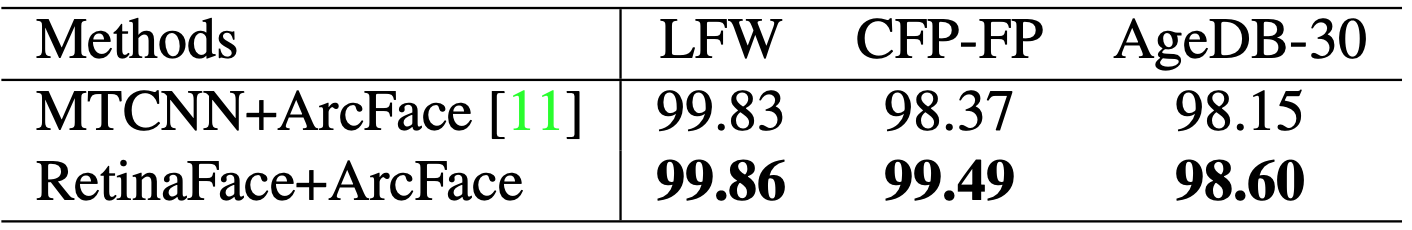
\includegraphics[width=10cm] {images/retinaface_results_2}
        \caption{Mô hình RetinaFace nguyên bản giúp cải thiện kết quả của bài toán nhận diện danh tính khuôn mặt\index{nhận diện danh tính khuôn mặt}. (Nguồn: \cite{deng2020retinaface})}
        \label{fig:retinaface_results_2}
    \end{figure}

    \noindent
    \textbf{\textit{Chi tiết kiến trúc của nhánh xác định đối tượng}} \\
    Nhánh xác định đối tượng\index{nhánh xác định đối tượng} cũng sử dụng kiến trúc FPN nhằm trích xuất đặc trưng của ảnh đầu vào với nhiều kích thước bản đồ đặc trưng\index{bản đồ đặc trưng} khác nhau.
    Hơn nữa, tương tự như RetinaFace \cite{deng2020retinaface}, nhánh xác định đối tượng\index{nhánh xác định đối tượng} đưa các bản đồ đặc trưng\index{bản đồ đặc trưng} này qua các Context Module \cite{najibi2017ssh} nhằm thu thập thêm các thông tin về background\index{background} xung quanh trước khi đưa ra dự đoán về hộp giới hạn\index{hộp giới hạn} chứa khuôn mặt.
    Ý tưởng sử dụng các khối Context Module \cite{najibi2017ssh} tỏ ra khá hiệu quả khi áp dụng với bài toán nhận diện khuôn mặt.

    \begin{figure}[H]
        \centering
        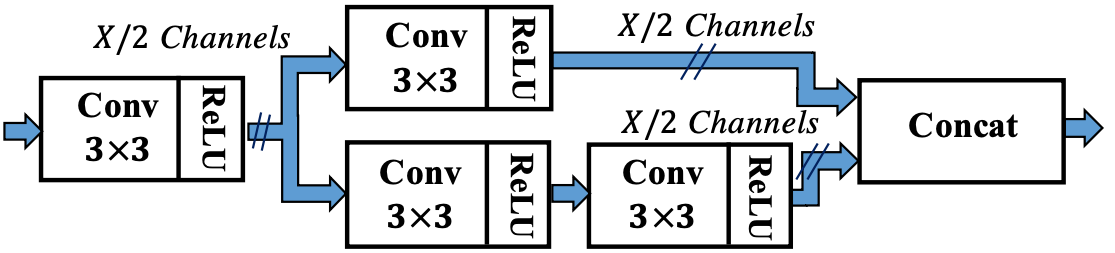
\includegraphics[width=10cm] {images/retinaface_context_module}
        \caption{Chi tiết kiến trúc nguyên bản của khối Context Module (Nguồn: \cite{najibi2017ssh})}
        \label{fig:retinaface_context_module}
    \end{figure}

    \noindent
    Đặc biệt trong việc định vị các mặt nhỏ, vì khi những thông tin về background\index{background} xung quanh như thân người sẽ có vai trò quan trọng giúp mô hình học tốt hơn.
    Trong kiến trúc của nhánh xác định đối tượng\index{nhánh xác định đối tượng}, ba bản đồ đặc trưng\index{bản đồ đặc trưng} \textit{{${P}_{3}, {P}_{4}, {P}_{5}$}} của FPN của mô hình xương sống được đưa qua ba khối Context Module độc lập.
    Mỗi khối Context Module gồm ba khối Conv nối tiếp nhau, nhưng bản đồ đặc trưng\index{bản đồ đặc trưng} đầu ra của mỗi khối Conv đều được concat lại với nhau để tạo ra bản đồ đặc trưng\index{bản đồ đặc trưng} cuối cùng của cả khối Context Module. \\

    \begin{figure}[H]
        \centering
        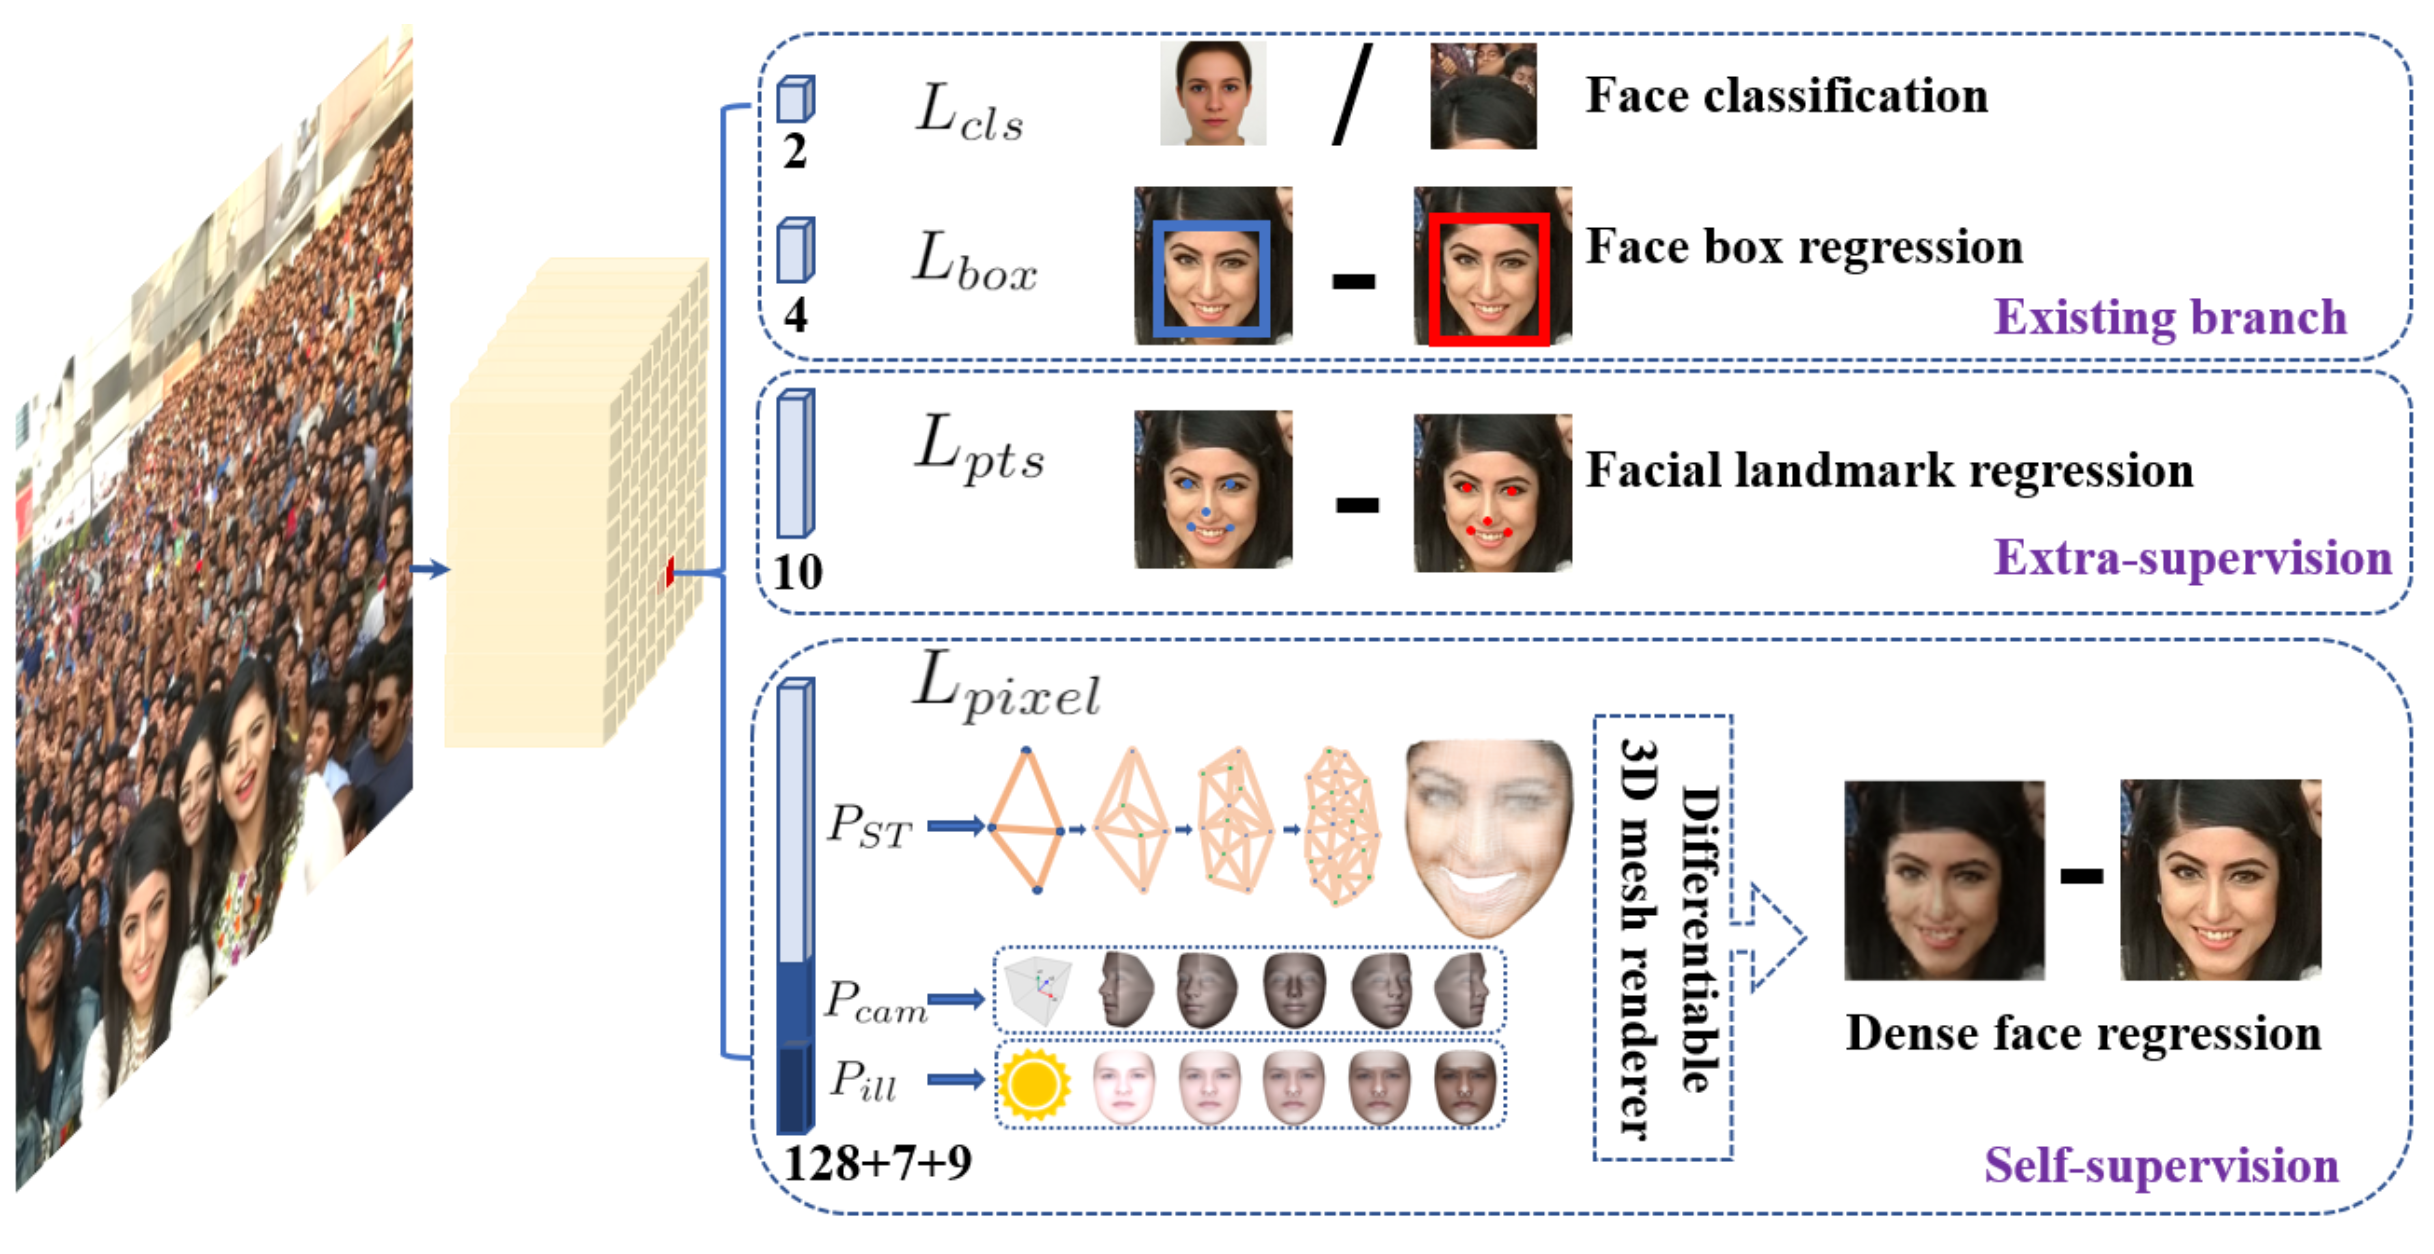
\includegraphics[width=10cm] {images/retinaface_loss_funcs}
        \caption{Ý tưởng các hàm mất mát đa nhiệm vụ\index{hàm mất mát đa nhiệm vụ} của mô hình RetinaFace. Ngoài hàm mất mát học tự giám sát\index{hàm mất mát học tự giám sát} \cite{zhou2019dense, genova2018unsupervised}, các hàm mất mát còn lại được kế thừa cho mô hình RetinaFocus (Nguồn: \cite{deng2020retinaface})}
        \label{fig:retinaface_loss_funcs}
    \end{figure}

    \noindent
    \textbf{\textit{Hàm mất mát đa nhiệm vụ}} \\
    Đầu ra nhánh xác định đối tượng\index{nhánh xác định đối tượng} của RetinaFocus gồm toạ độ của hộp giới hạn\index{hộp giới hạn} dự đoán của mô hình, toạ độ của landmarks của khuôn mặt và xác suất mà hộp giới hạn\index{hộp giới hạn} dự đoán đó chứa khuôn mặt.
    Các đầu ra này tiếp tục được đưa vào hàm mất mát đa nhiệm vụ\index{hàm mất mát đa nhiệm vụ}, tương tự như mô hình RetinaFace \cite{deng2020retinaface}. \\
    Cụ thể, trong quá trình huấn luyện mô hình, với mỗi khu vực mỏ neo\index{khu vực mỏ neo}, nhánh xác định đối tượng\index{nhánh xác định đối tượng} của mô hình RetinaFocus tối ưu hàm mất mát đa nhiệm vụ\index{hàm mất mát đa nhiệm vụ} dưới đây:

    \begin{equation}
        \begin{split}
        L  & =  L_{cls}(p_i, p^{*}_i) + \lambda_1 p^{*}_i L_{box}(t_i, t^{*}_i) + \lambda_2 p^{*}_i L_{pts} (l_i, l^{*}_i).\\
        \end{split}
        \label{eq:retinaface_loss}
    \end{equation}

    \noindent
    trong đó: \\
    - Các trọng số $\lambda_1, \lambda_2$ được cấu hình mặc định theo mô hình RetinaFace \cite{deng2020retinaface} lần lượt là 0.25, 0.1 và 0.01. Các trọng số này đóng vai trò giúp cân bằng tỷ lệ của các thành phần $L_{cls}$, $L_{box}$ và $L_{pts}$ của hàm mất mát đa nhiệm vụ\index{hàm mất mát đa nhiệm vụ}. \\
    - Hàm mất mát phân lớp mặt: \\
    $L_{cls}(p_i, p^{*}_i)$ với $p_i$ là xác suất mà mô hình dự đoán một khu vực mỏ neo\index{khu vực mỏ neo} có chứa là khuôn mặt hay không.
    Ta có $p^{*}_i = 1$ nếu khu vực mỏ neo\index{khu vực mỏ neo} đó chứa khuôn mặt còn $p^{*}_i = 0$ nếu khu vực mỏ neo\index{khu vực mỏ neo} đó không chứa khuôn là mặt. \\
    - Hàm mất mát hồi quy định vị vị trí của hộp giới hạn\index{hộp giới hạn}: \\
    $L_{box}(t_i, t^{*}_i)$ với $t_i=\{t_x, t_y, t_w, t_h\}_i$ và $t^{*}_i=\{t^{*}_x, t^{*}_y, t^{*}_w, t^{*}_h\}_i$ lần lượt là bộ bốn tham số đại diện cho toạ độ của khu vực mỏ neo\index{khu vực mỏ neo} mà mô hình dự đoán là mặt và hộp giới hạn\index{hộp giới hạn} groundtruth\index{groundtruth} từ bộ dữ liệu.
    (x là toạ độ x của điểm góc trái trên, y là toạ độ y của điểm góc trái trên, w là chiều rộng của hộp giới hạn\index{hộp giới hạn} và h là chiều cao của hộp giới hạn\index{hộp giới hạn}). \\
    - Hàm mất mát hồi quy định vị vị trí của landmarks: \\
    $L_{pts} (l_i, l^{*}_i)$ với $l_i=\{l_{x_1}, l_{y_1}, \dots , l_{x_5}, l_{y_5}\}_i$ và $l^{*}_i=\{l^{*}_{x_1}, l^{*}_{y_1}, \dots , l^{*}_{x_5}, l^{*}_{y_5}\}_i$ lần lượt là bộ mười tham số đại diện cho toạ độ của năm landmarks mà mô hình dự đoán ứng với mỗi hộp giới hạn\index{hộp giới hạn} dự đoán và năm groundtruth\index{groundtruth} landmarks của mỗi groundtruth\index{groundtruth} hộp giới hạn\index{hộp giới hạn} từ bộ dữ liệu. \\

    \noindent
    \textbf{\textit{So sánh giữa mô hình RetinaFace nguyên bản và nhánh xác định đối tượng của mô hình RetinaFocus}} \\
    Mặc dù kế thừa kiến trúc mô hình RetinaFace nguyên bản để xây dựng nhánh xác định đối tượng của mô hình RetinaFocus, tuy nhiên, vẫn có những sự khác biệt nhất định.

    \begin{figure}[H]
        \centering
        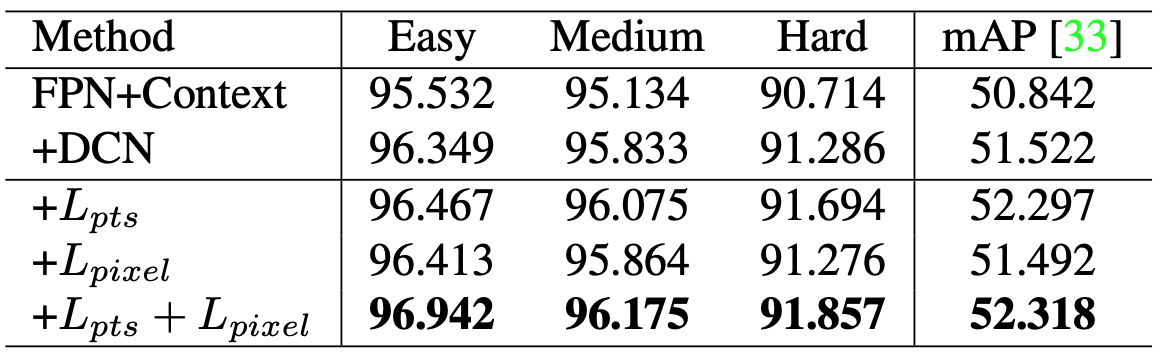
\includegraphics[width=10cm] {images/retinaface_results_1}
        \caption{Vai trò của lớp DCN và hàm mất mát học tự giám sát đối với kết quả của mô hình RetinaFace nguyên bản trên bộ dữ liệu WIDER FACE (Nguồn: \cite{deng2020retinaface})}
        \label{fig:retinaface_results_1}
    \end{figure}

    \noindent
    Đầu tiên, mô hình RetinaFace nguyên bản sử dụng các lớp Conv được kế thừa từ mô hình DCN \cite{dai2017deformable}, giúp nâng cao độ chính xác của mô hình hơn so với lớp Conv thông thường.
    Trong khi đó, nhánh xác định đối tượng của mô hình RetinaFocus không sử dụng lớp DCN này. \\
    Tiếp theo, mô hình RetinaFace bổ sung thêm các hàm mất mát học tự giám sát\index{hàm mất mát học tự giám sát} \cite{zhou2019dense, genova2018unsupervised} vào hàm mất mát đa nhiệm vụ\index{hàm mất mát đa nhiệm vụ} chung giúp cải thiện độ chính xác khi nhận diện khuôn mặt.
    Nhánh xác định đối tượng của mô hình RetinaFocus không sử dụng bổ trợ các hàm mất mát này. \\
    Cuối cùng, về mặt kiến trúc của mô hình RetinaFace nguyên bản sử dụng các bản đồ đặc trưng\index{bản đồ đặc trưng} $C_6, P_5, P_4, P_3$ và $P_2$ làm đầu vào cho các khối Context Module \cite{najibi2017ssh}.
    Trong khi đó, nhánh xác định đối tượng của mô hình RetinaFocus chỉ sử dụng các bản đồ đặc trưng\index{bản đồ đặc trưng} $P_5, P_4$ và $P_3$ làm đầu vào cho các khối Context Module \cite{najibi2017ssh}. \\
    Những sự khác biệt này được đưa ra dựa trên điều kiện trong quá trình lập trình cài đặt mô hình RetinaFocus.
}
    \retinaface

    \subsubsection{Mô hình AutoFocus}
    \def\focusbranch{
    Nhánh tập trung đối tượng\index{nhánh tập trung đối tượng} của RetinaFocus được xây dựng dựa trên mô hình AutoFocus \cite{najibi2019autofocus}, một mô hình giải quyết bài toán xử lý ảnh chất lượng cao rất hiệu quả.
    Ý tưởng của AutoFocus \cite{najibi2019autofocus} hướng đến việc loại bỏ những điểm ảnh\index{điểm ảnh} dư thừa mà mô hình phải xử lý trong quá trình dự đoán nhưng vẫn giữ được ý tưởng về việc sử dụng Image Pyramids.
    Theo kết quả được báo cáo tại \cite{najibi2019autofocus}, mô hình AutoFocus đạt độ chính xác tương đương với mô hình SNIPER \cite{singh2018sniper} (một mô hình sử dụng chiến lược dự đoán Image Pyramids) với tốc độ xử lý 6.4 ảnh/giây (so sánh với 2.5 ảnh/giây của mô hình SNIPER).

    \begin{figure}[H]
        \centering
        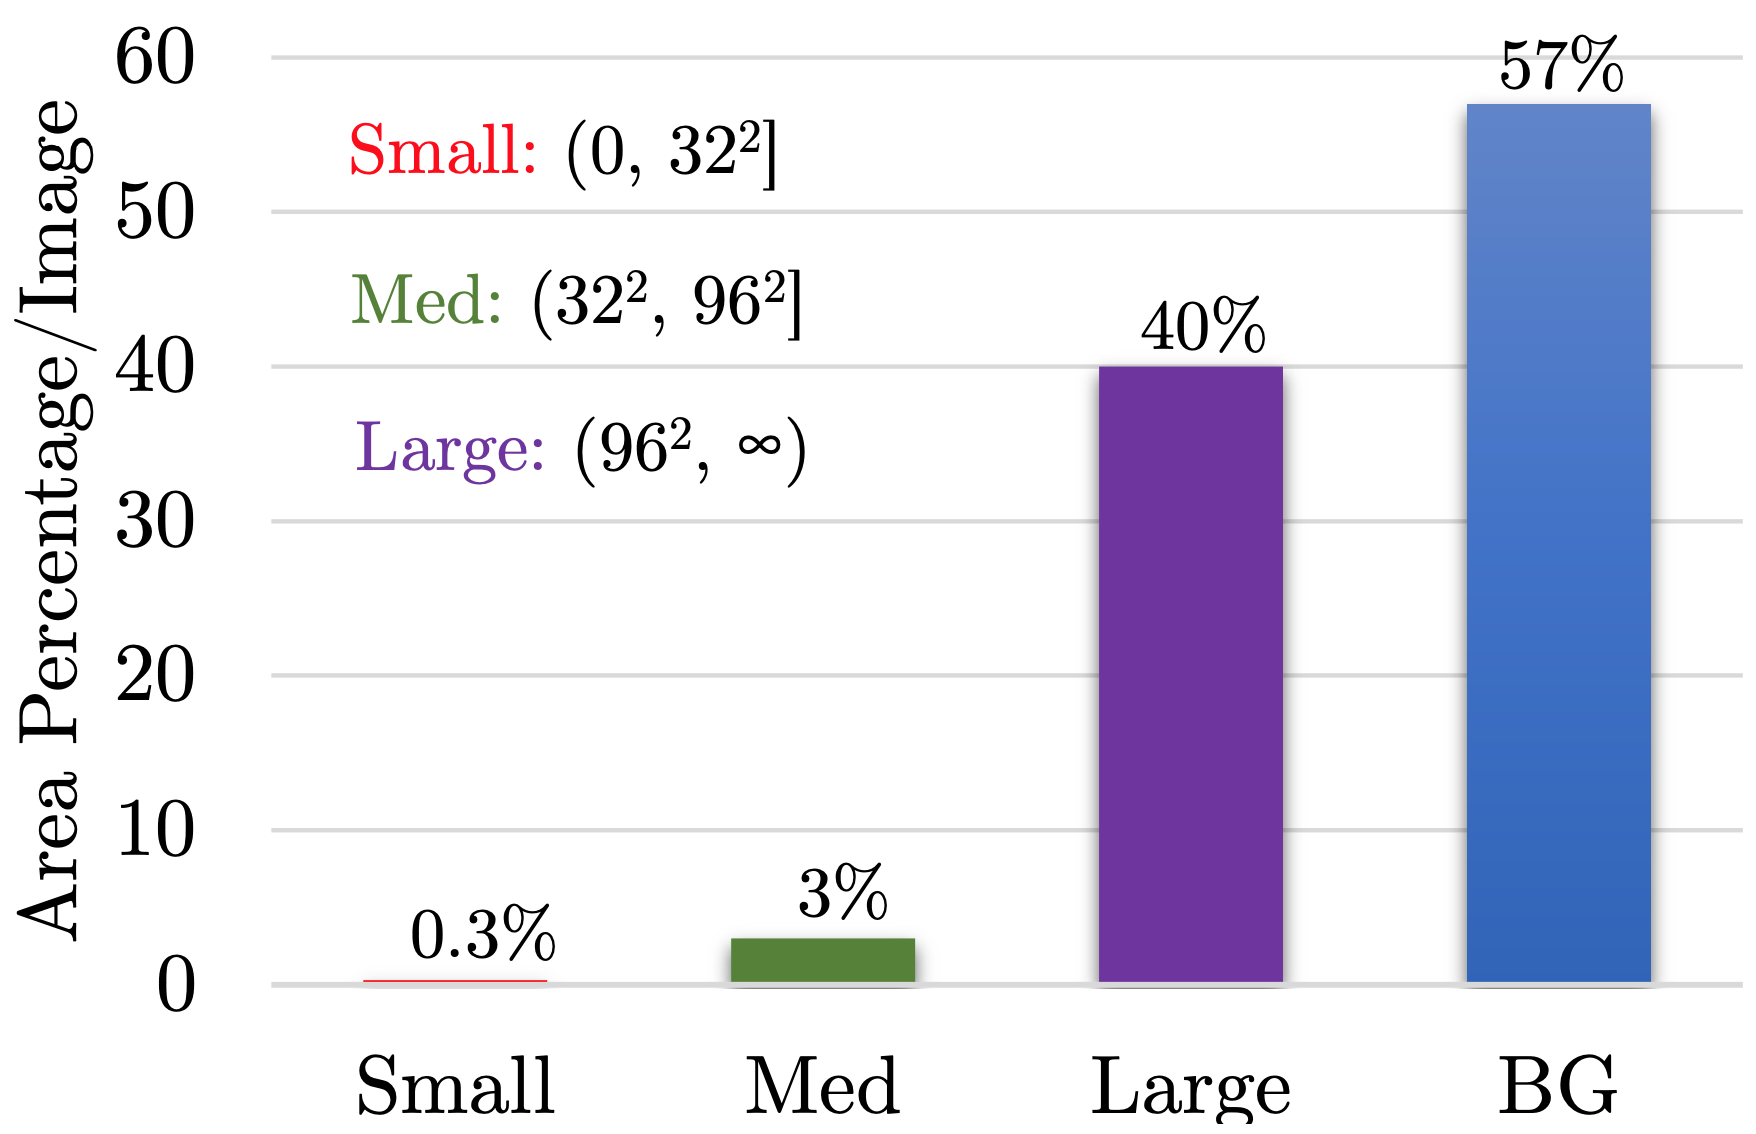
\includegraphics[width=8cm] {images/autofocus_compare_fg_bg}
        \caption{Thống kê về tỷ lệ diện tích của các vùng chứa đối tượng nhỏ (kích thước nhỏ hơn 32 pixels), vừa (kích thước từ 32 đến 96 pixels) và lớn (kích thước lớn hơn 96 pixels) so sánh với diện tích của background của ảnh trên bộ dữ liệu COCO \cite{lin2014microsoft} (Nguồn: \cite{najibi2019autofocus})}
        \label{fig:autofocus_compare_fg_bg}
    \end{figure}

    \noindent
    Ý tưởng của nhánh tập trung đối tượng\index{nhánh tập trung đối tượng} được thiết kế nhằm dự đoán những khu vực đáng chú ý ở trên ảnh và loại bỏ những khu vực khả năng cao không chứa đối tượng ở những kích thước ảnh lớn hơn, từ đó, tiết kiệm được rất nhiều chi phí tính toán trong quá trình dự đoán của mô hình.

    \noindent
    Dựa trên mô hình AutoFocus \cite{najibi2019autofocus}, nhánh tập trung đối tượng\index{nhánh tập trung đối tượng} của RetinaFocus gồm hai thành phần là \textit{Thuật toán Focus Pixel} và \textit{Thuật toán sinh Focus Chips}.
    Ngoài ra, bổ sung thêm \textit{Thuật toán Focus Stacking} vào nhánh xác định đối tượng\index{nhánh xác định đối tượng}. \\

    \noindent
    \textbf{\textit{Thuật toán Focus Pixel}} \\
    Tương tự như trong mô hình AutoFocus \cite{najibi2019autofocus}, thuật toán Focus Pixel là thuật toán giúp chúng ta có thể xác định được vị trí khu vực có khả năng chứa đối tượng và cần zoom trên ảnh.
    Ý tưởng của thuật toán Focus Pixel  dựa trên việc khi ta đưa đầu vào một ảnh có kích thước $X \times Y$ qua một khối Conv, bản đồ đặc trưng\index{bản đồ đặc trưng} mà ta thu được có kích thước $X' \times Y'$, trong đó: $X' = \lceil \frac{X}{s} \rceil$, $Y' = \lceil \frac{Y}{s} \rceil$, và $s$ là stride của cả khối Conv.
    Từ đó ta có thể ngầm hiểu rằng một điểm ảnh\index{điểm ảnh} trên bản đồ đặc trưng\index{bản đồ đặc trưng} có kích thước $X' \times Y'$ đại diện cho một khu vực có kích thước $s \times s$ trên ảnh đầu vào.

    \begin{figure}[H]
        \centering
        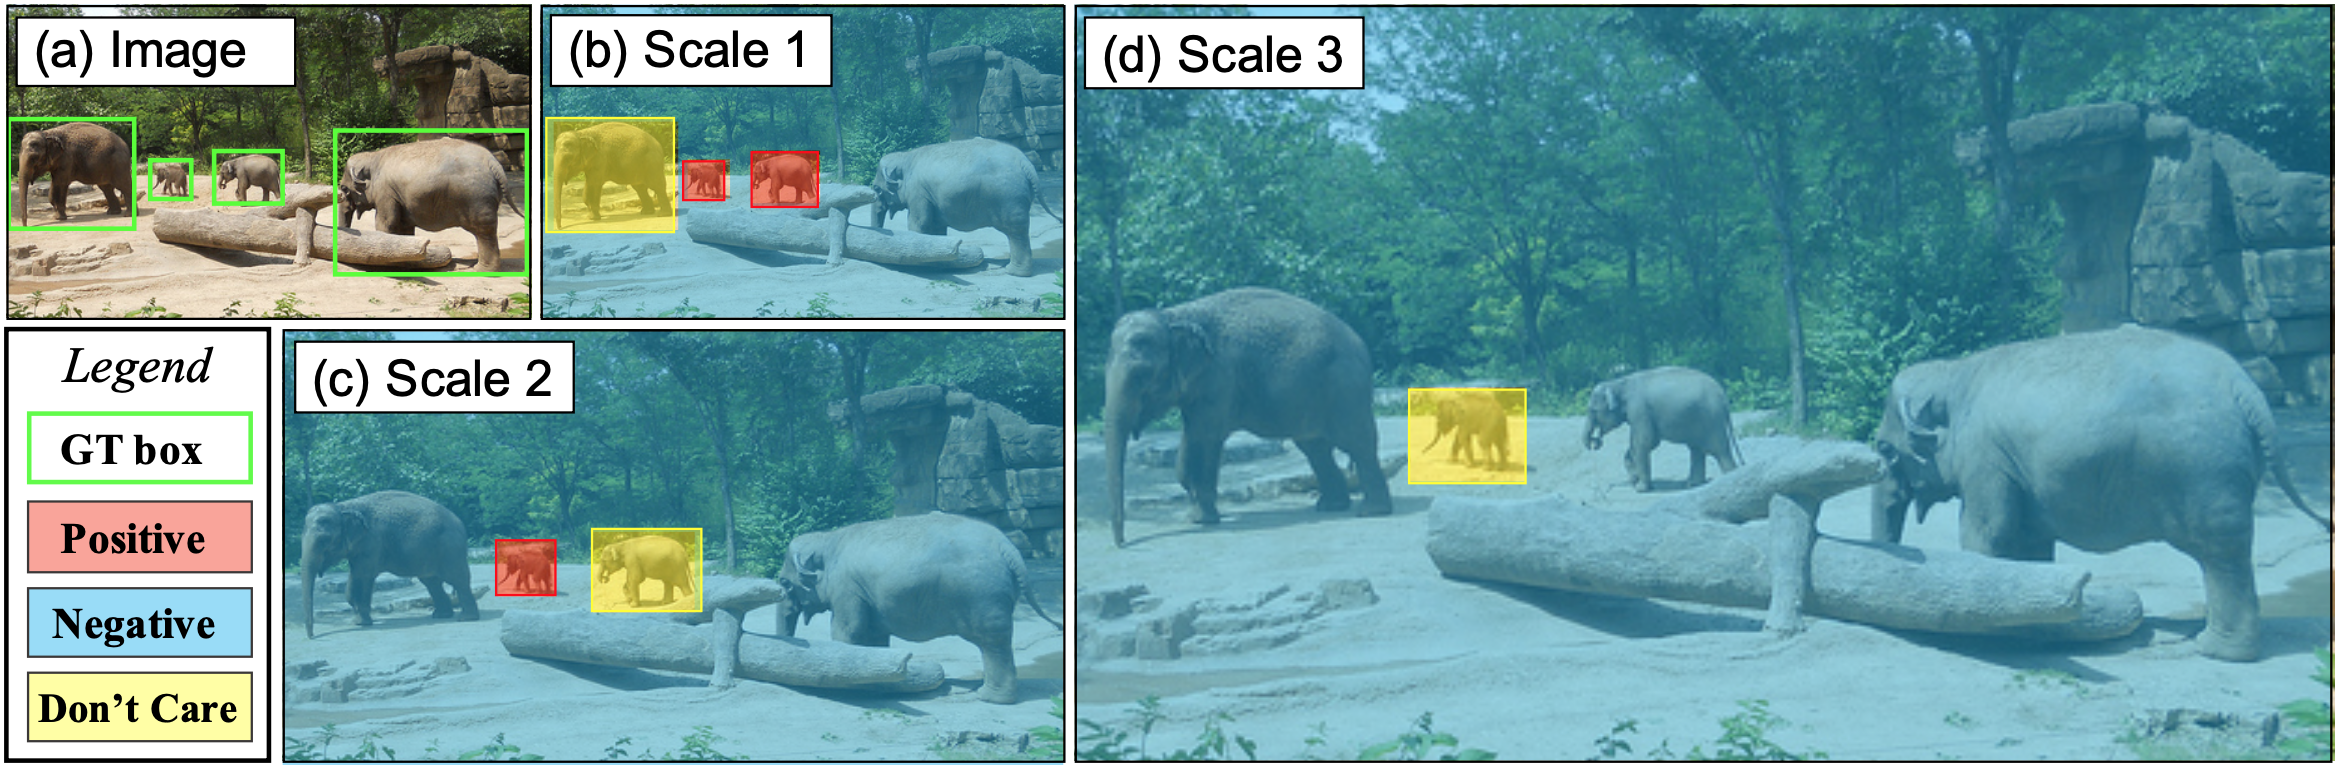
\includegraphics[width=15cm] {images/autofocus_focus_pixel}
        \caption{Các nhóm hộp giới hạn khác nhau trong thuật toán Focus Pixel (Nguồn: \cite{najibi2019autofocus})}
        \label{fig:autofocus_focus_pixel}
    \end{figure}

    \noindent
    Cụ thể, Focus Pixel  xác định các điểm ảnh\index{điểm ảnh} trên mask là các \textit{điểm ảnh cần được focus} nếu như điểm ảnh\index{điểm ảnh} đó có overlap với grountruth hộp giới hạn\index{hộp giới hạn} của đối tượng có kích thước nhỏ.
    Tiếp theo, các điểm ảnh\index{điểm ảnh} trên mask là các \textit{điểm ảnh không cần quan tâm} nếu như điểm ảnh\index{điểm ảnh} đó có overlap với groundtruth\index{groundtruth} hộp giới hạn\index{hộp giới hạn} của đối tượng có kích thước lớn hoặc rất nhỏ.
    Cuối cùng, các \textit{điểm ảnh không cần được focus} trên mask là các điểm ảnh\index{điểm ảnh} còn lại.

    \[l = 
        \begin{cases}
            1, & IoU\index{IoU}(GT, l) > 0, a < \sqrt{GTArea} < b \\
            -1, & IoU\index{IoU}(GT, l) > 0, \sqrt{GTArea} < a  \\
            -1, & IoU\index{IoU}(GT, l) > 0, b < \sqrt{GTArea} < c  \\
            0, & \text{otherwise}
        \end{cases}
    \]

    \noindent
    trong đó: \\
    - $IoU\index{IoU}(GT, l)$ là chỉ số IoU\index{IoU} giữa khu vực $s \times s$ và groundtruth\index{groundtruth} hộp giới hạn\index{hộp giới hạn} của đối tượng trên ảnh đầu vào. \\
    - $GTArea$ là diện tích của groundtruth\index{groundtruth} hộp giới hạn\index{hộp giới hạn} của đối tượng trên ảnh đầu vào. \\
    Nếu một khu vực $s \times s$ overlap với nhiều groundtruth\index{groundtruth} hộp giới hạn\index{hộp giới hạn} của đối tượng, thì điểm ảnh\index{điểm ảnh} đó được ưu tiên là một Focus Pixel .

    \noindent
    Trong các thí nghiệm mà nhóm tác giả của AutoFocus \cite{najibi2019autofocus} thực hiện, nhóm tác giả sử dụng các tham số $a = 5, b = 64, c = 90$.
    Các groundtruth\index{groundtruth} hộp giới hạn\index{hộp giới hạn} có kích thước từ $5 \times 5$ đến $64 \times 64$ pixels là các hộp giới hạn\index{hộp giới hạn} cần được tập trung (nhánh tập trung đối tượng sẽ được học và dự đoán các hộp giới hạn thuộc kích thước này), các groundtruth\index{groundtruth} hộp giới hạn\index{hộp giới hạn} có kích thước dưới $5 \times 5$ pixels hoặc từ $64 \times 64$ đến $90 \times 90$ pixels là các hộp giới hạn\index{hộp giới hạn} không cần quan tâm và các groundtruth\index{groundtruth} hộp giới hạn\index{hộp giới hạn} có kích thước trên $90 \times 90$ pixels là các hộp giới hạn\index{hộp giới hạn} không cần được tập trung (nhánh tập trung đối tượng sẽ được không được học các hộp giới hạn thuộc kích thước này).
    
    \noindent
    Tuy nhiên, để nhánh tập trung đối tượng\index{nhánh tập trung đối tượng} hoạt động hiệu quả, ta cần xây dựng được bộ tham số phù hợp với bộ dữ liệu và nhánh xác định đối tượng\index{nhánh xác định đối tượng}.

    \begin{figure}[H]
        \centering
        \subfigure[]{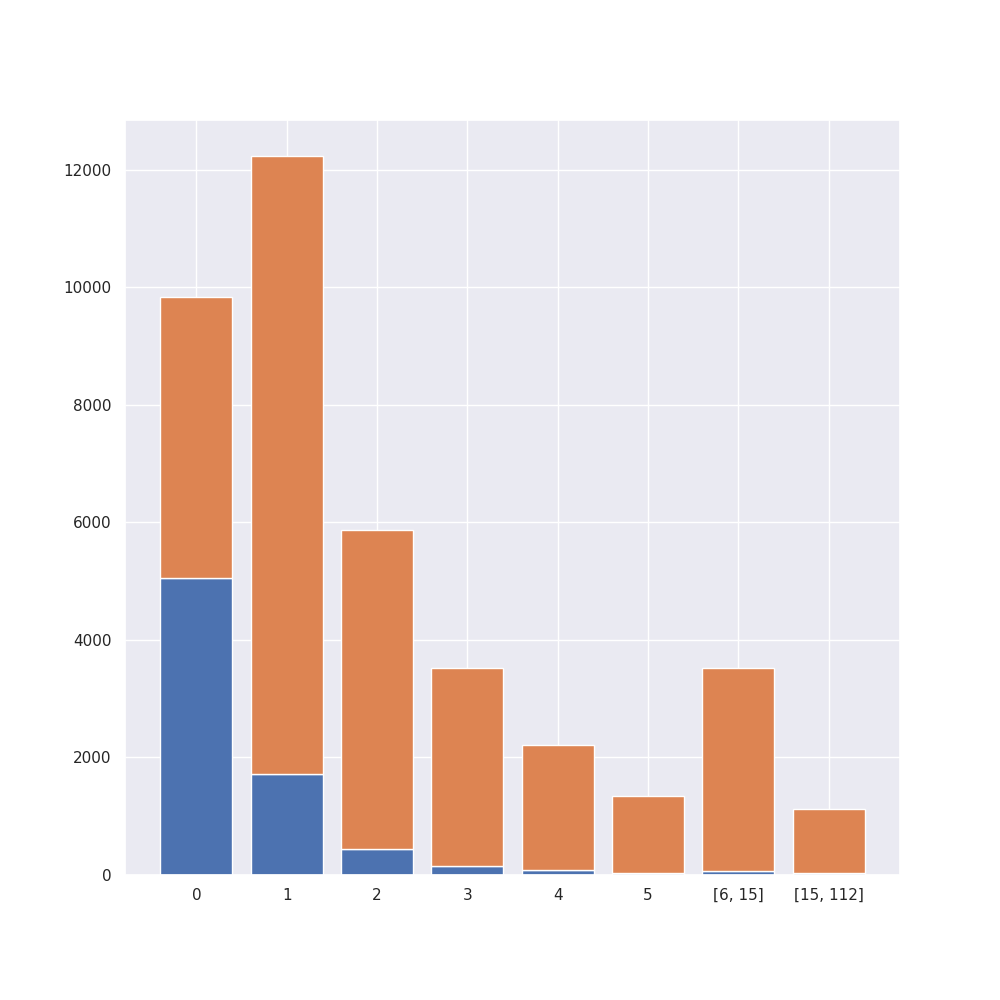
\includegraphics[width=7.3cm, trim={2.5cm 0cm 1.7cm 3.3cm}, clip]{images/retinafocus_iou_50_compare}} 
        \subfigure[]{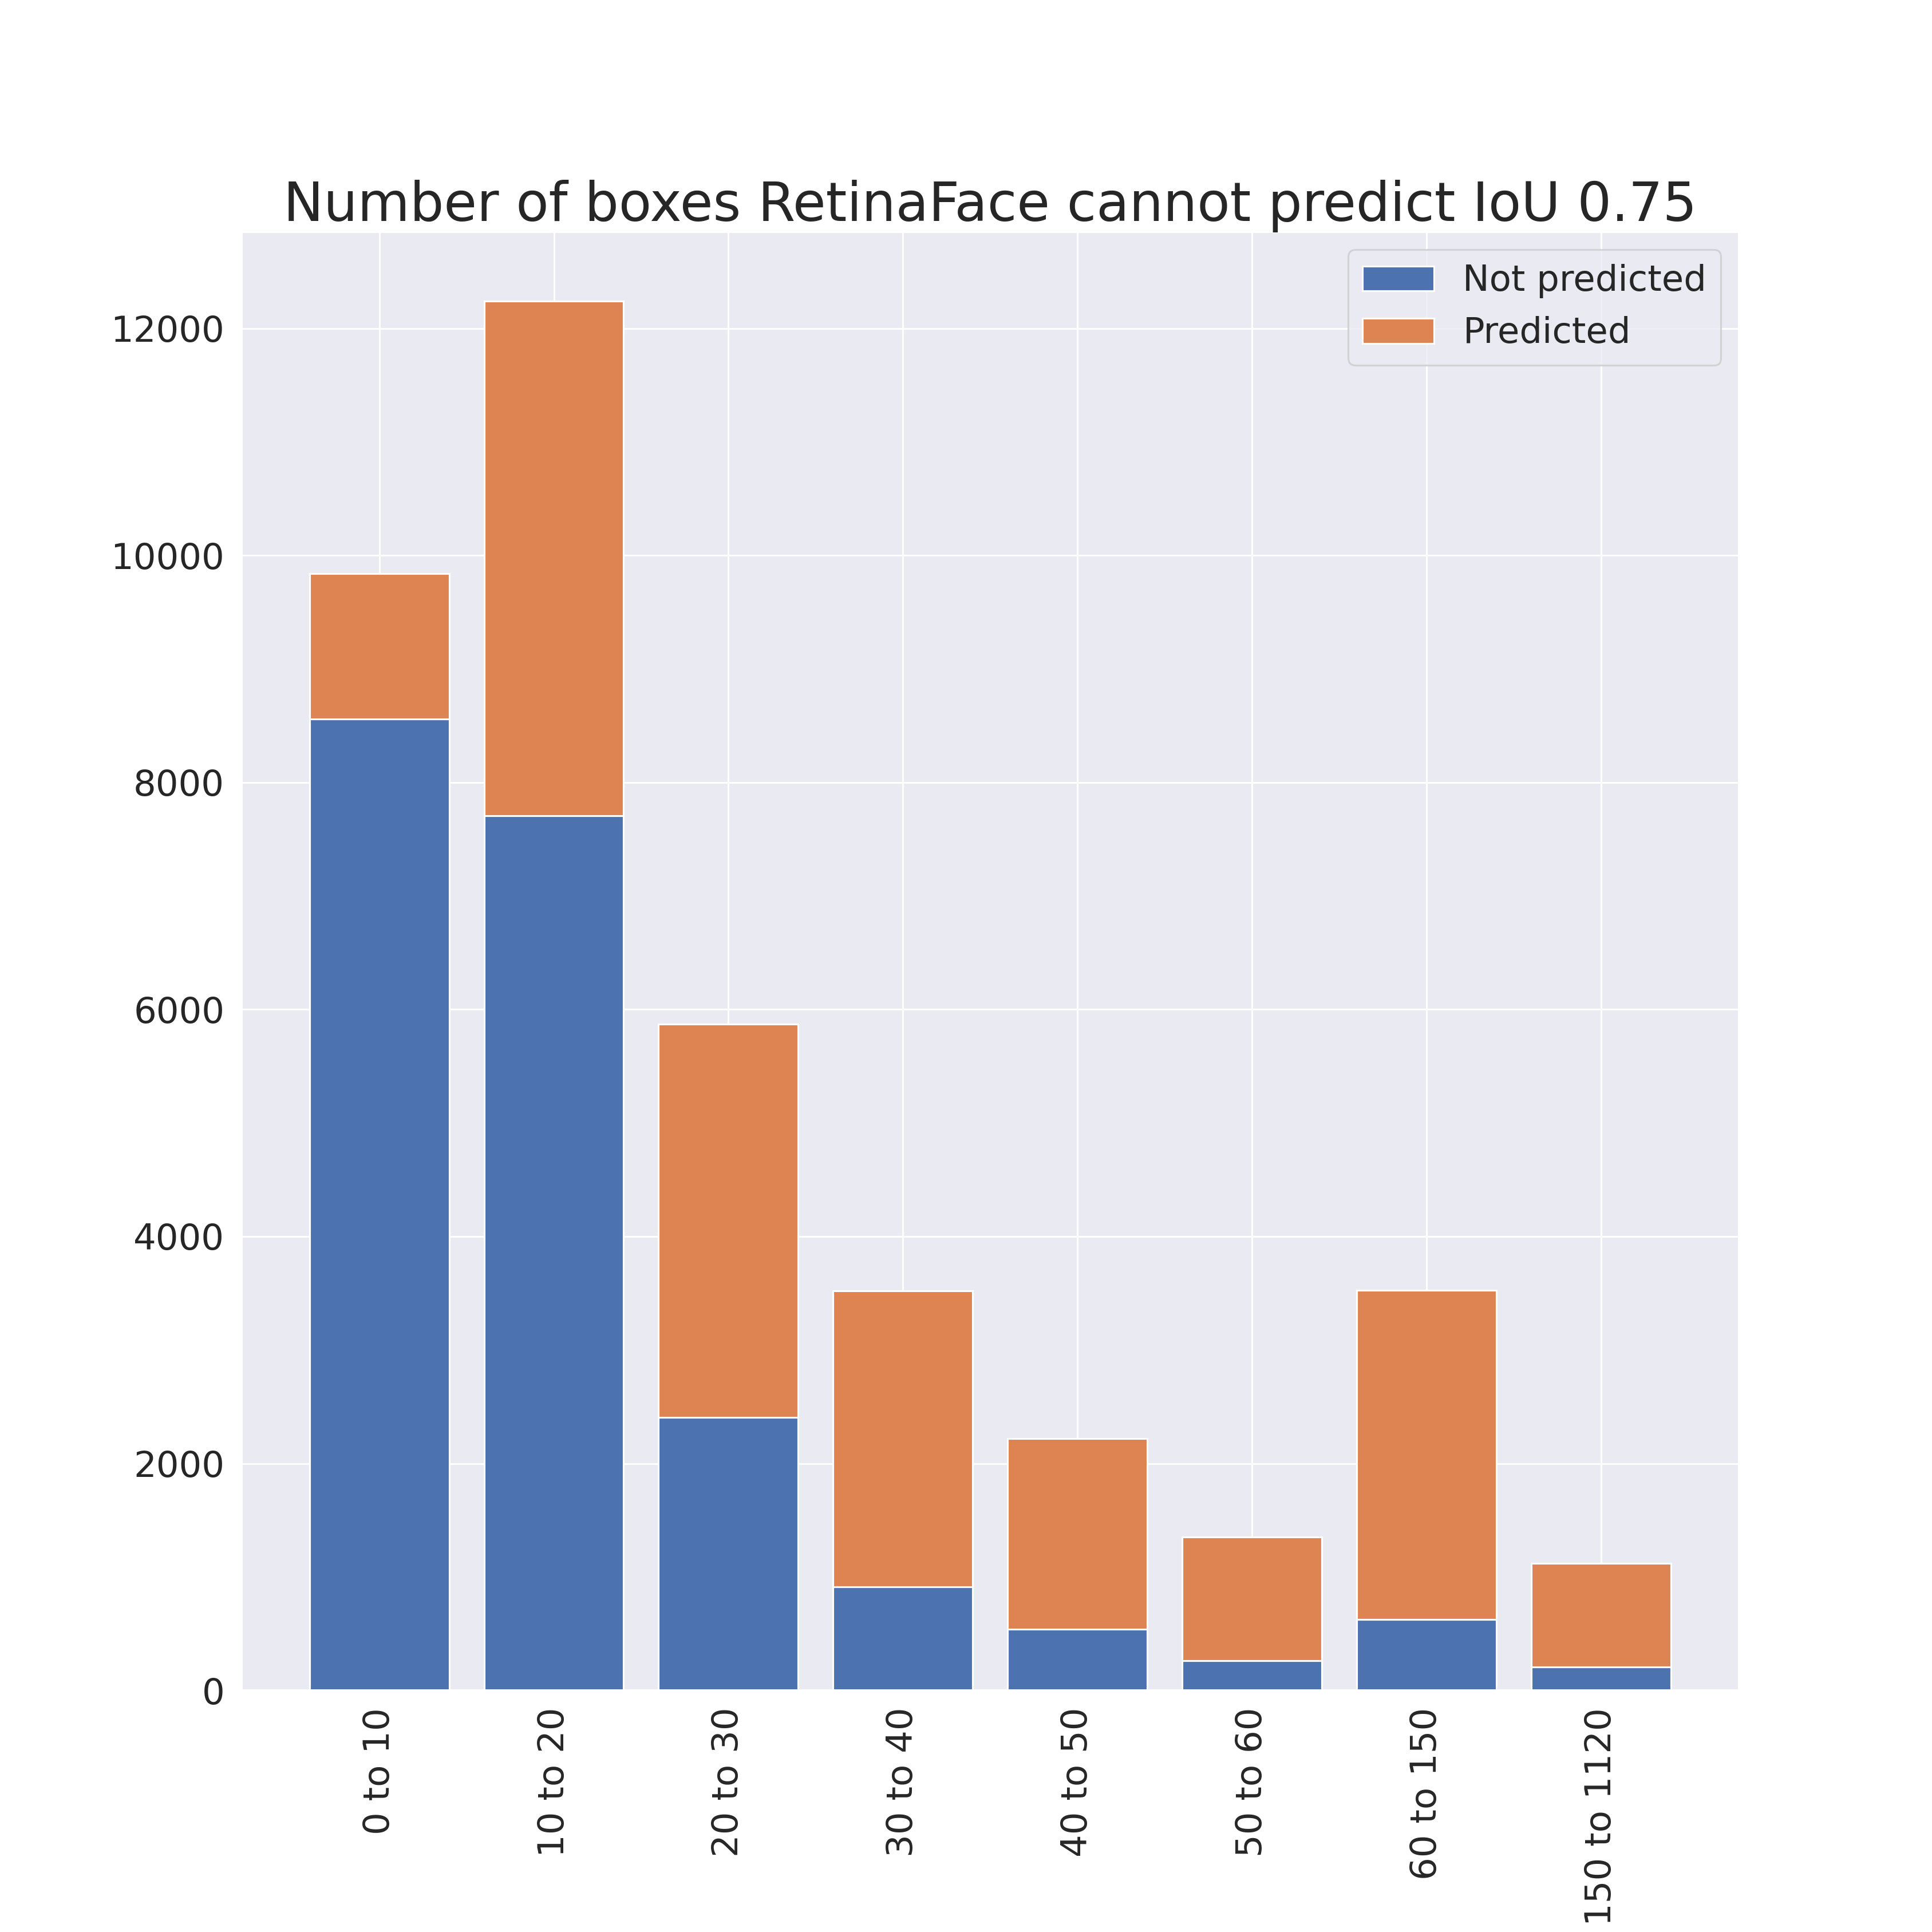
\includegraphics[width=7.3cm, trim={2.5cm 0cm 1.7cm 3.3cm}, clip]{images/retinafocus_iou_75_compare}} 
        \subfigure[]{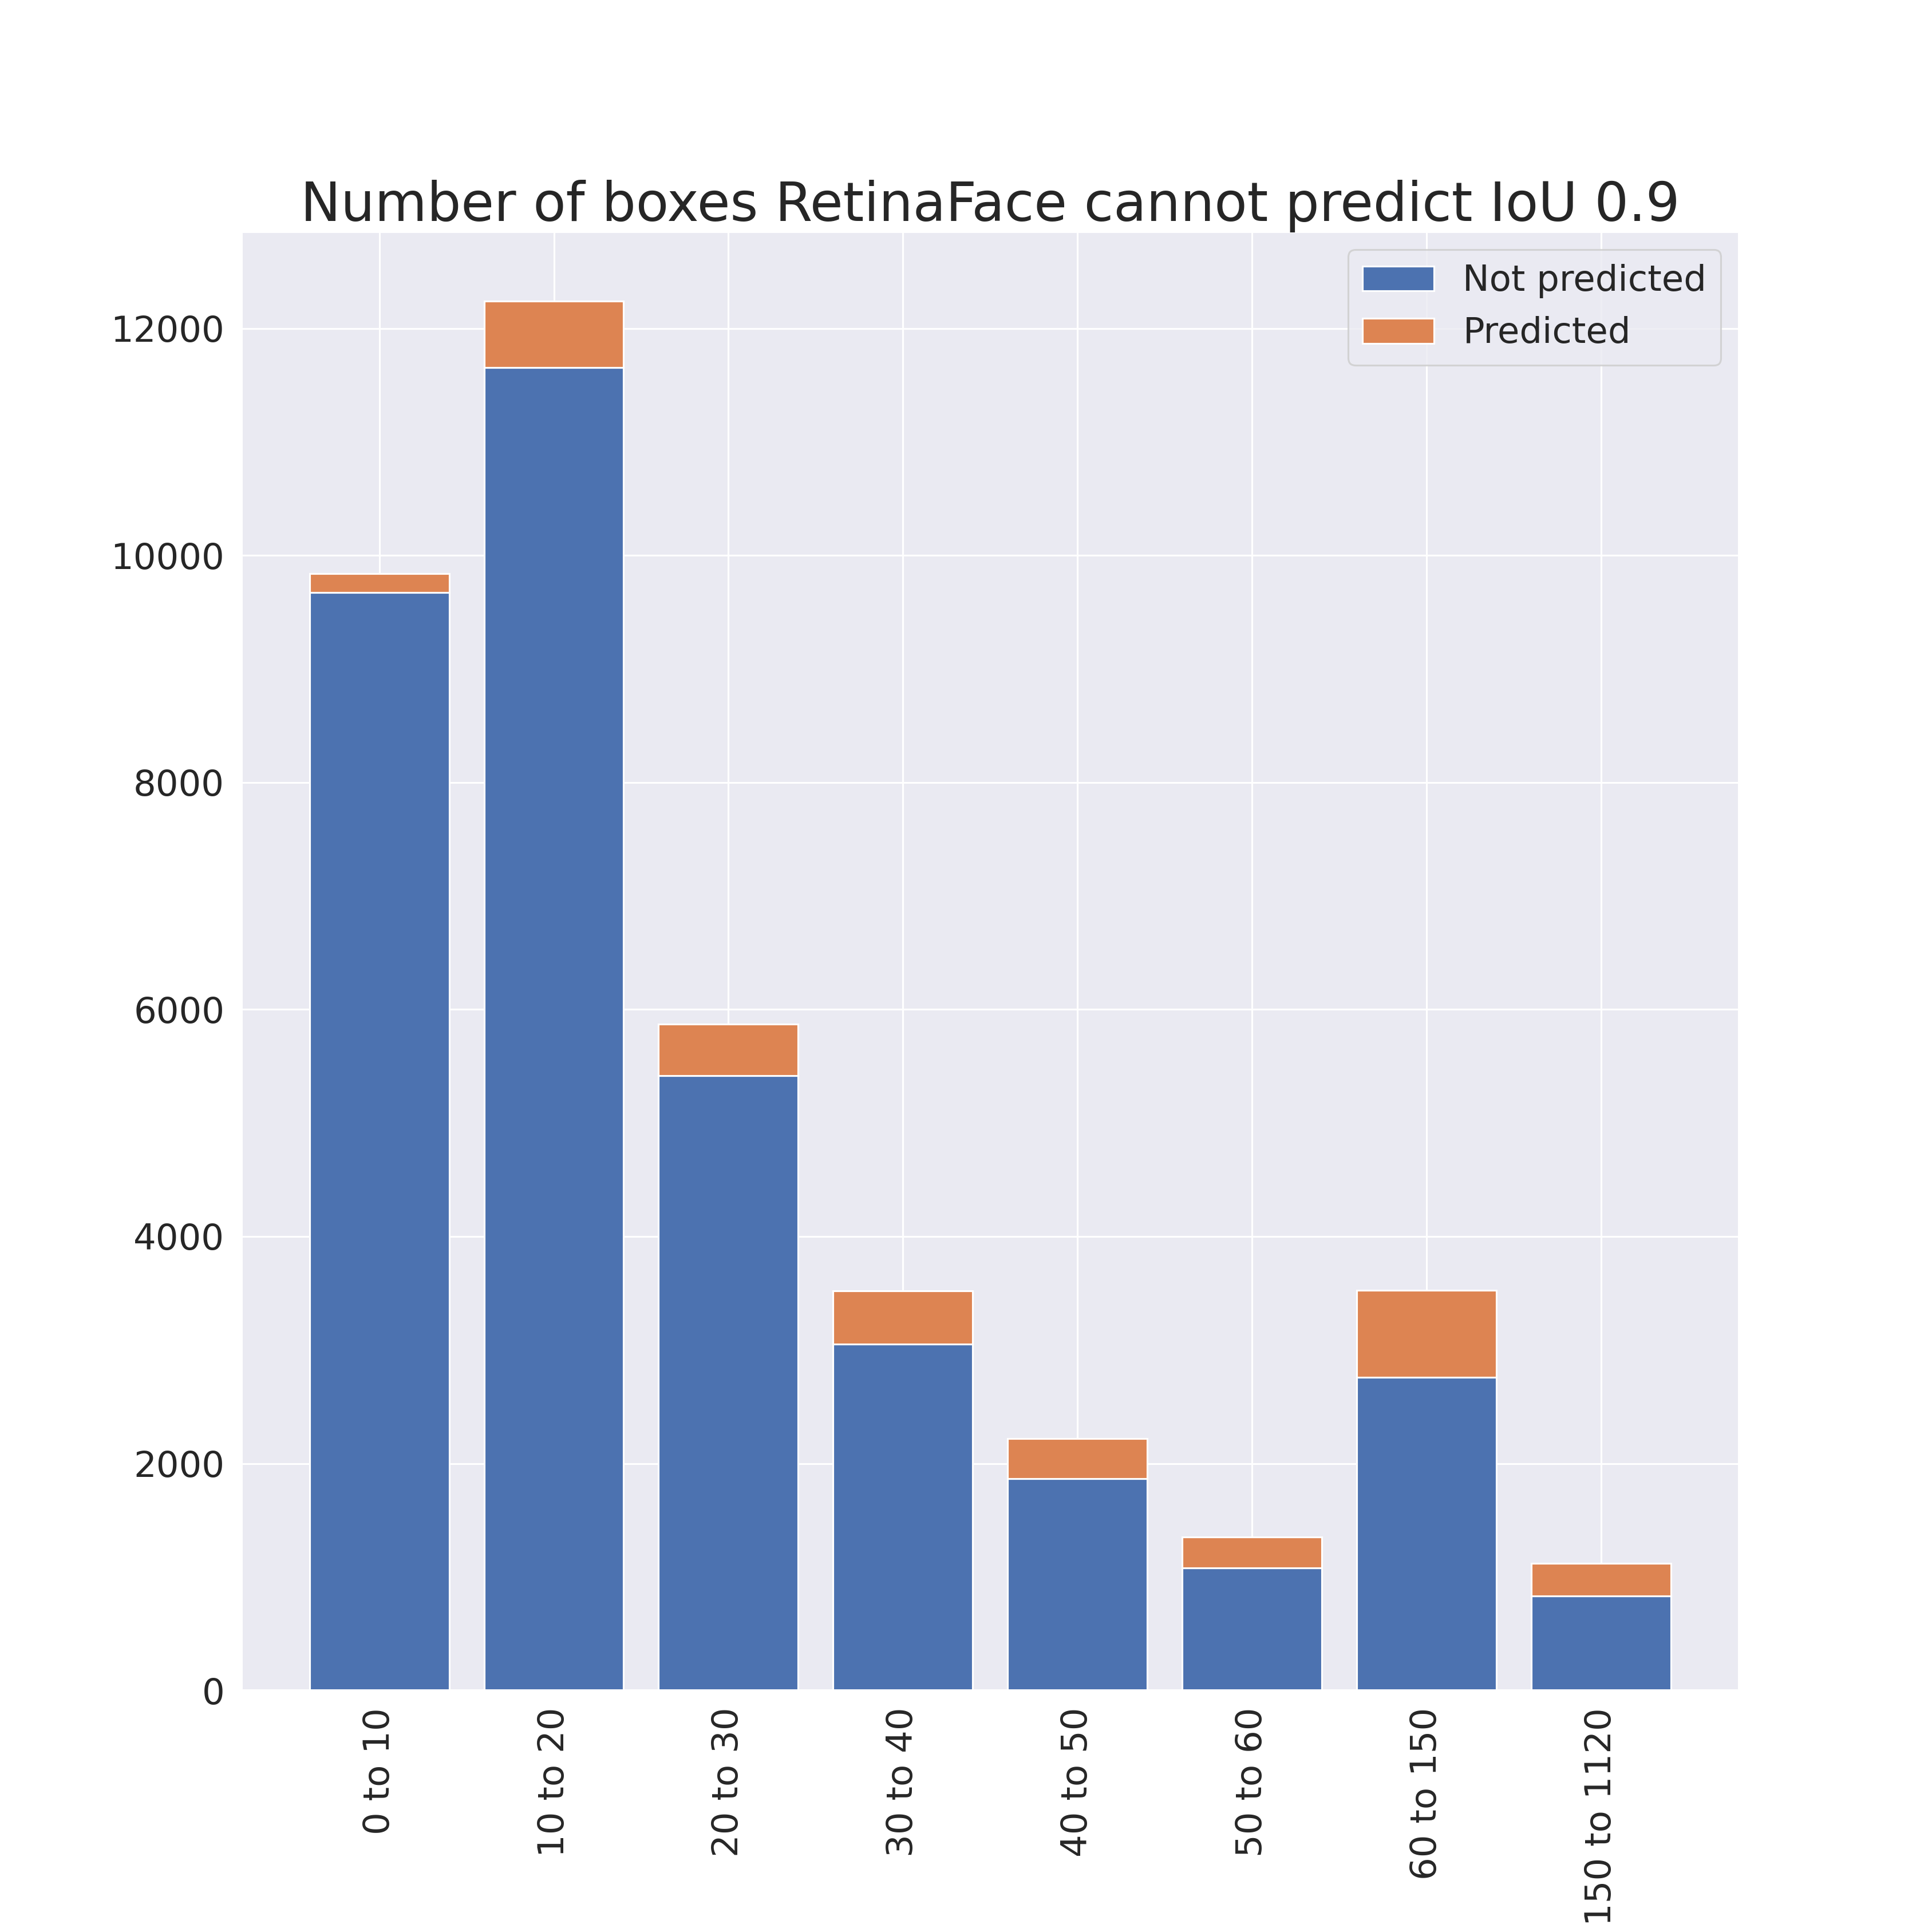
\includegraphics[width=7.3cm, trim={2.5cm 0cm 1.7cm 3.3cm}, clip]{images/retinafocus_iou_90_compare}} 
        \caption{So sánh số lượng hộp giới hạn\index{hộp giới hạn} trên từng nhóm kích thước mà mô hình RetinaFace dự đoán ra và không dự đoán ra tương ứng với IoU\index{IoU} 0.5 (a), IoU\index{IoU} 0.75 (b), IoU\index{IoU} 0.9 (c)}
        \label{fig:retinafocus_iou_compare}
    \end{figure}

    \noindent
    Để xây dựng được bộ tham số này, ta cần phân tích điểm yếu của nhánh xác định đối tượng\index{nhánh xác định đối tượng} trên bộ dữ liệu WIDER FACE.
    Từ những điểm yếu, ta lựa chọn bộ tham số của nhánh tập trung đối tượng\index{nhánh tập trung đối tượng} nhằm giúp cho nhánh tập trung đối tượng\index{nhánh tập trung đối tượng} xác định được những vùng mà nhánh xác định đối tượng\index{nhánh xác định đối tượng} dự đoán yếu và zoom in giúp nhánh xác định đối tượng\index{nhánh xác định đối tượng} dự đoán chính xác hơn.

    \noindent
    Trong hình \ref{fig:retinafocus_iou_compare_percent}, trên cả ba mức IoU\index{IoU}, tỷ lệ số lượng hộp giới hạn\index{hộp giới hạn} mà mô hình RetinaFace không dự đoán ra đối với nhóm các hộp giới hạn\index{hộp giới hạn} nhỏ từ 0 điểm ảnh\index{điểm ảnh} đến 30 điểm ảnh\index{điểm ảnh} và đặc biệt là từ 0 điểm ảnh\index{điểm ảnh} đến 10 điểm ảnh\index{điểm ảnh} đều cao vượt trội so với các kích thước hộp giới hạn\index{hộp giới hạn} khác.

    \begin{figure}[H]
        \centering
        \subfigure[]{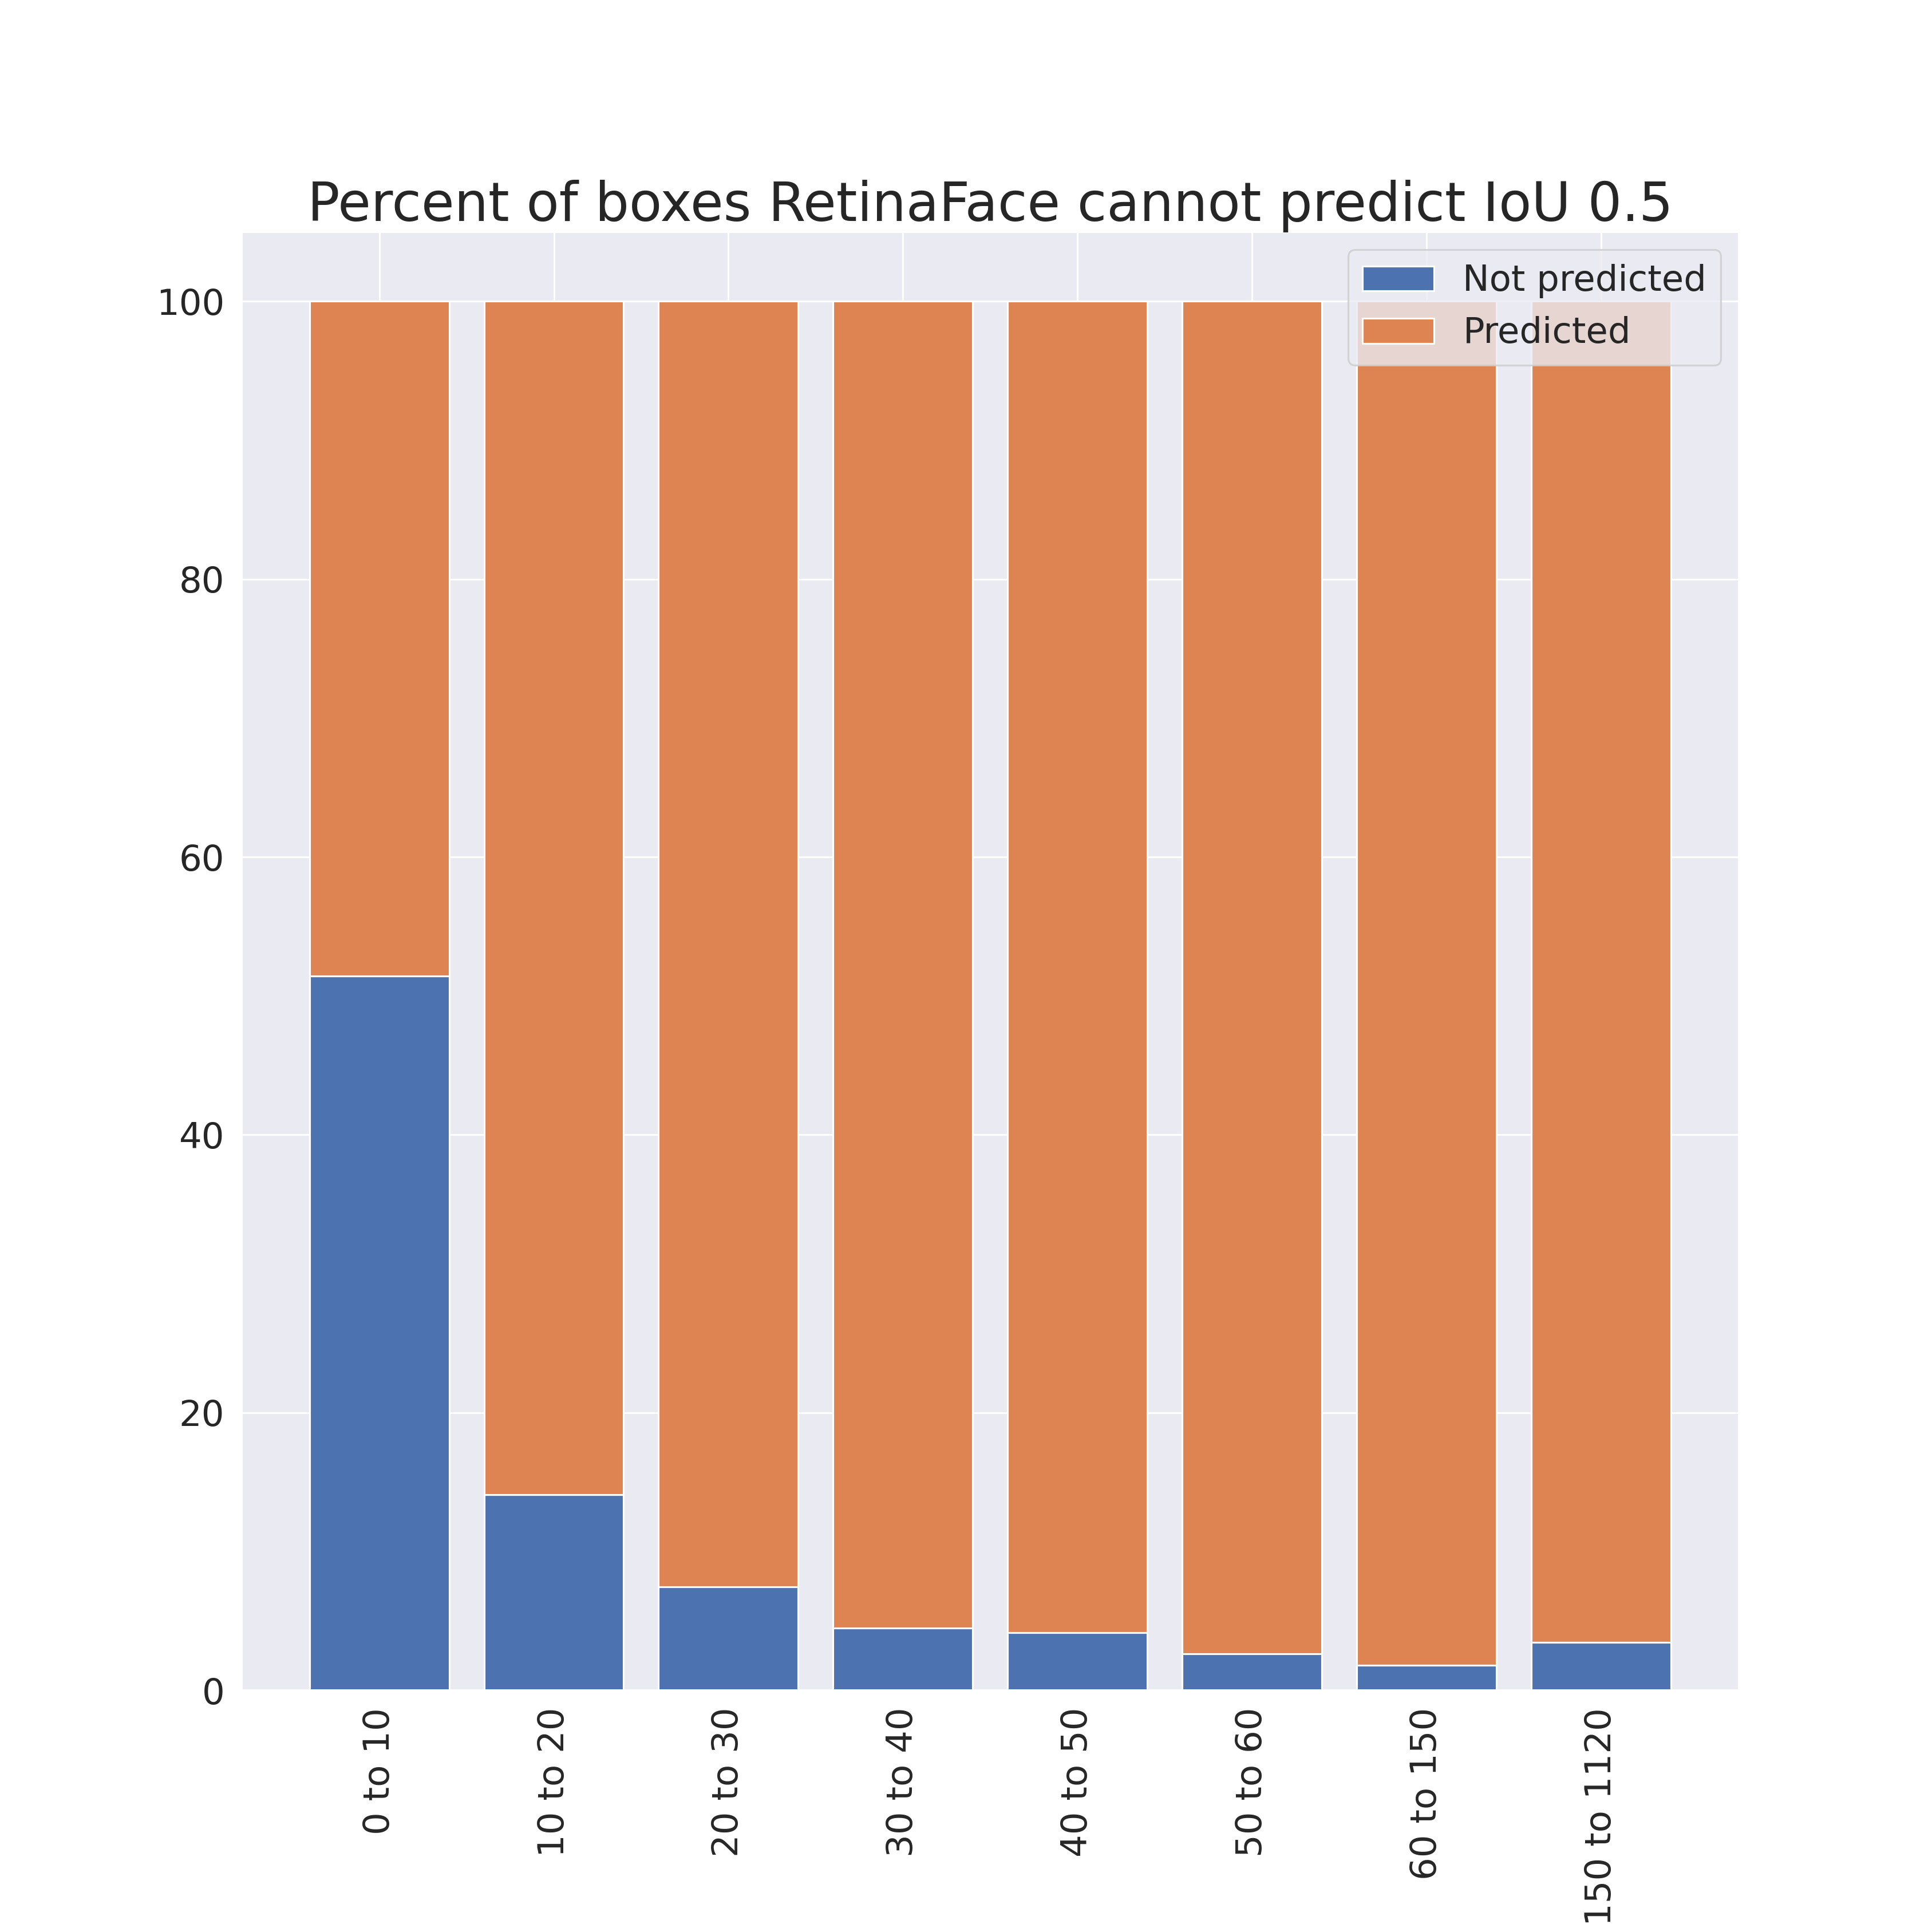
\includegraphics[width=7.3cm, trim={2.5cm 0cm 1.7cm 3.3cm}, clip]{images/retinafocus_iou_50_compare_percent}} 
        \subfigure[]{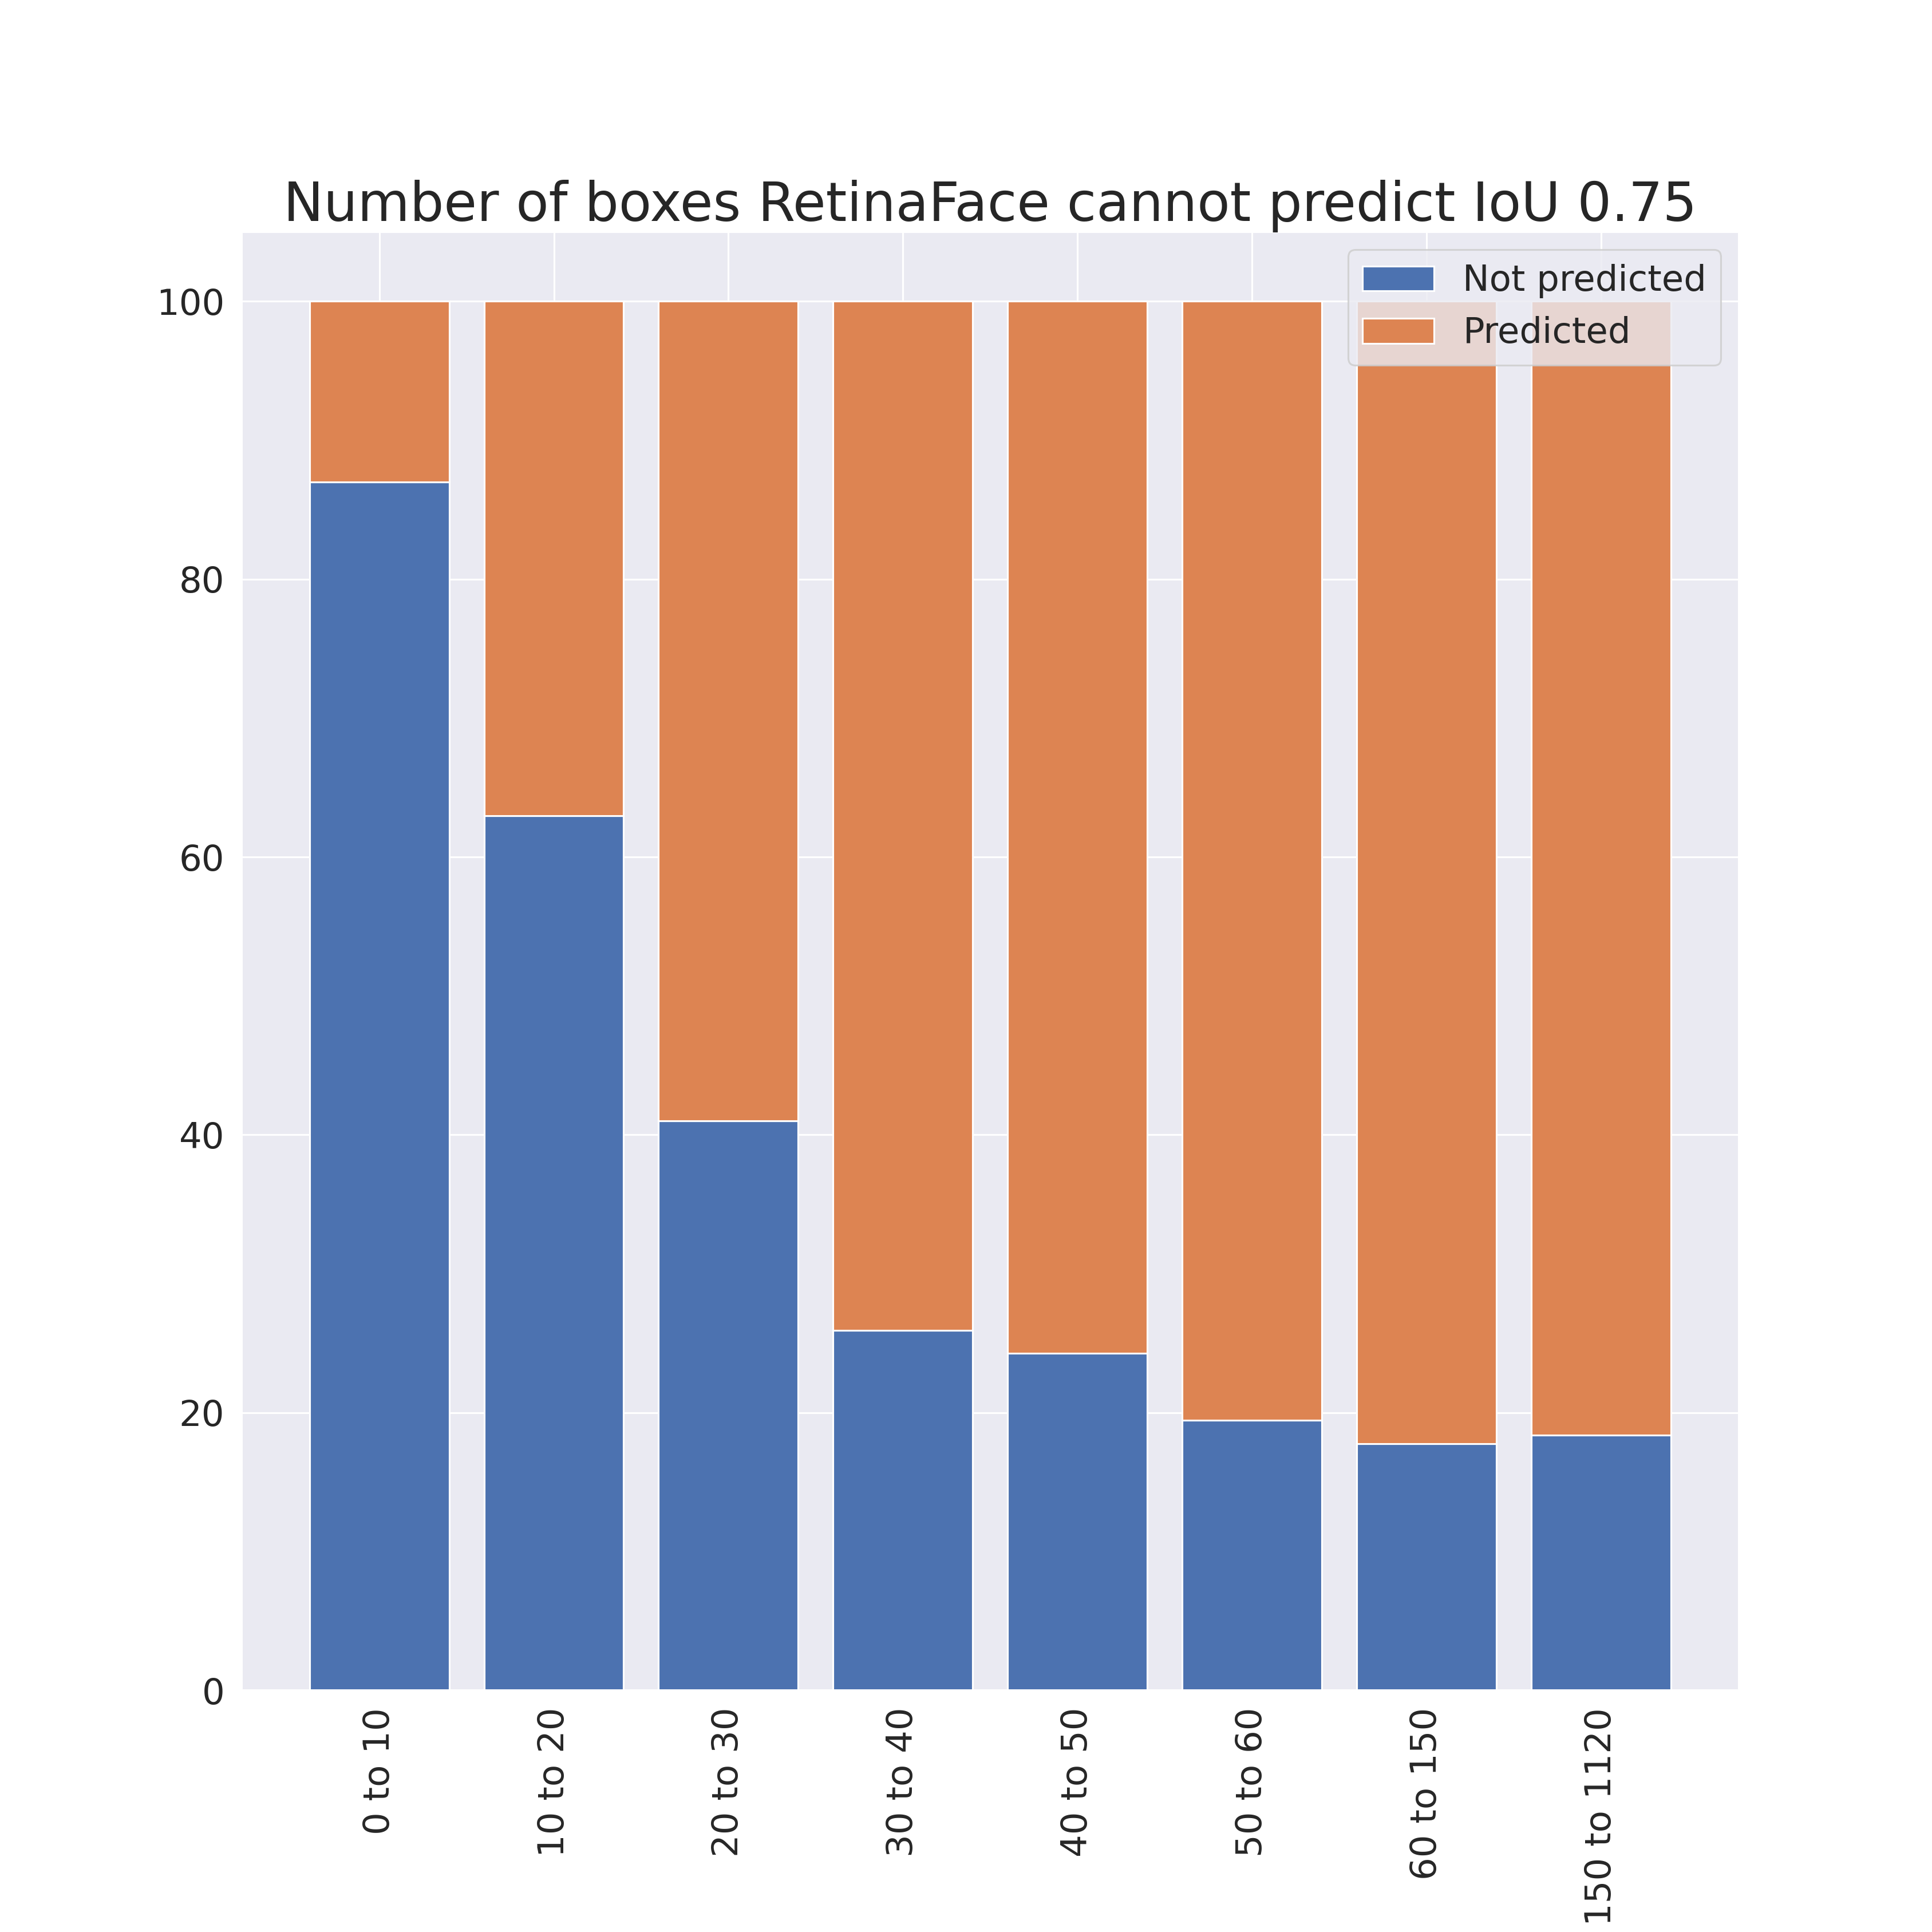
\includegraphics[width=7.3cm, trim={2.5cm 0cm 1.7cm 3.3cm}, clip]{images/retinafocus_iou_75_compare_percent}} 
        \subfigure[]{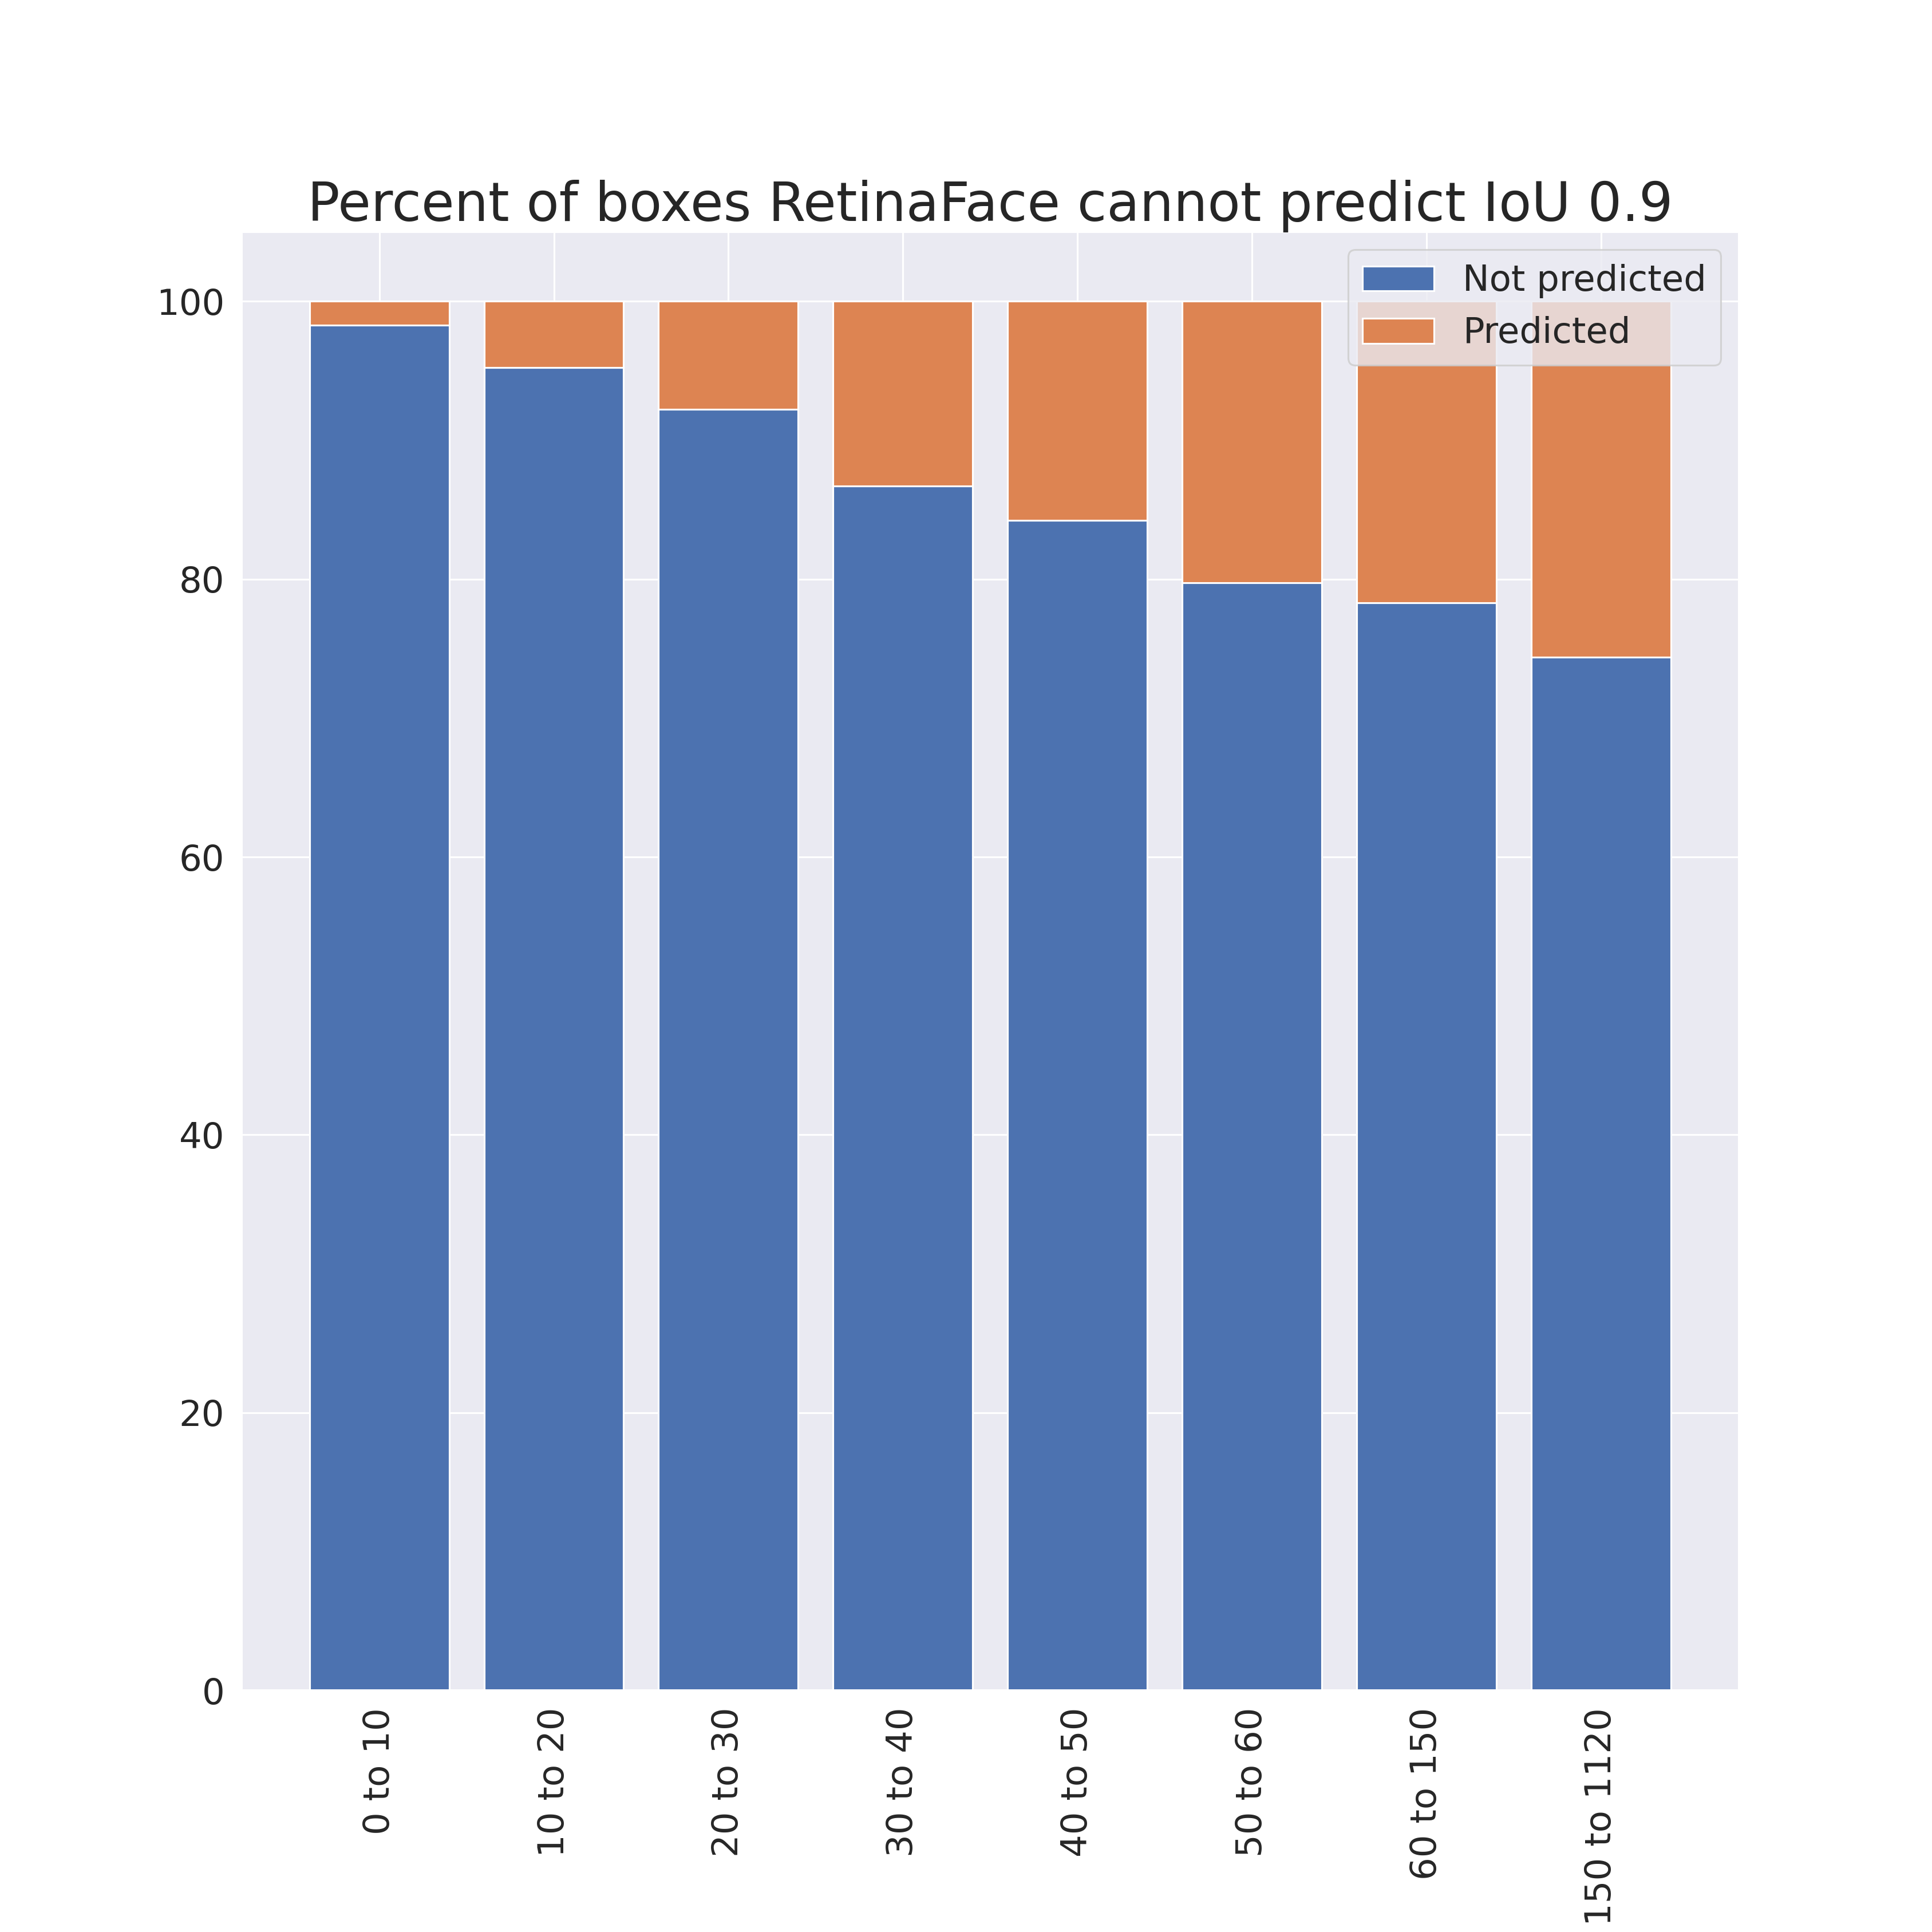
\includegraphics[width=7.3cm, trim={2.5cm 0cm 1.7cm 3.3cm}, clip]{images/retinafocus_iou_90_compare_percent}} 
        \caption{Tỷ lệ số lượng hộp giới hạn\index{hộp giới hạn} mà mô hình RetinaFace dự đoán ra và không dự đoán ra tương ứng với IoU\index{IoU} 0.5 (a), IoU\index{IoU} 0.75 (b), IoU\index{IoU} 0.9 (c) trên từng nhóm kích thước hộp giới hạn}
        \label{fig:retinafocus_iou_compare_percent}
    \end{figure}

    \noindent
    Cụ thể hơn, trong hình \ref{fig:retinafocus_iou_lower}, dù xét ở mức IoU\index{IoU} nào, thì các hộp giới hạn\index{hộp giới hạn} có kích thước nhỏ từ 0 đến 60 đều chiếm tổng tỷ lệ rất lớn, cụ thể, đối với IoU\index{IoU} 0.5 là 98.7\%, đối với IoU\index{IoU} 0.75 là 96\% và đối với IoU\index{IoU} 0.9 là 90.1\%.

    \noindent
    Hơn nữa, với kiến trúc của FPN như hình \ref{fig:retinafocus_architecture}, một hộp giới hạn\index{hộp giới hạn} có kích thước $4 \times 4$ ở ảnh đầu vào sẽ có tương ứng một khu vực có kích thước $2 \times 2$ ở bản đồ đặc trưng\index{bản đồ đặc trưng} ${C}_{2}$ và ${P}_{2}$, $1 \times 1$ ở bản đồ đặc trưng\index{bản đồ đặc trưng} ${C}_{3}$ và ${P}_{3}$ và gần như không còn thông tin ở các bản đồ đặc trưng\index{bản đồ đặc trưng} từ ${C}_{4}$ và ${P}_{4}$ trở đi.
    Điều này khiến cho các hộp giới hạn\index{hộp giới hạn} này trở thành các điểm dữ liệu nhiễu của nhánh tập trung đối tượng\index{nhánh tập trung đối tượng}, khiến cho việc học của nhánh tập trung đối tượng\index{nhánh tập trung đối tượng} bị giảm hiệu quả.

    \begin{figure}[H]
        \centering
        \subfigure[]{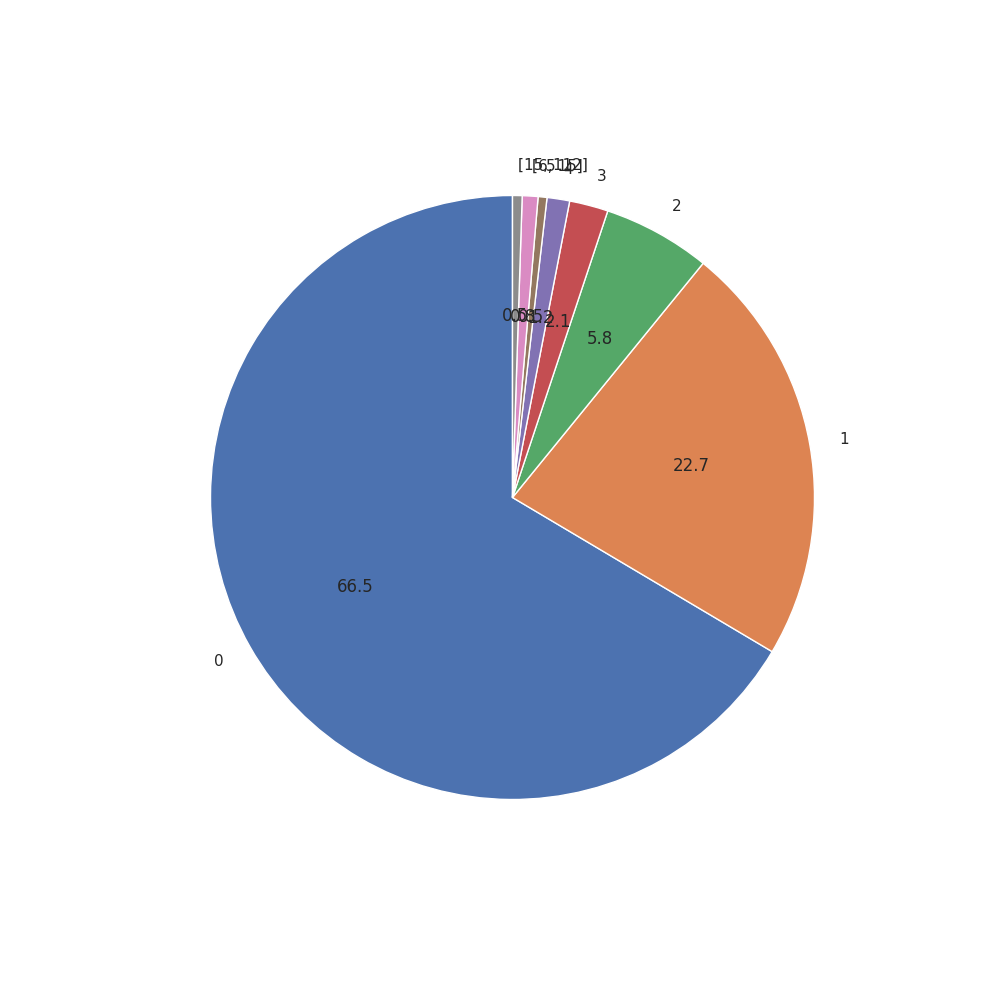
\includegraphics[width=7.3cm, trim={1.1cm 0cm 0.6cm 2cm}, clip]{images/retinafocus_iou_50_lower}} 
        \subfigure[]{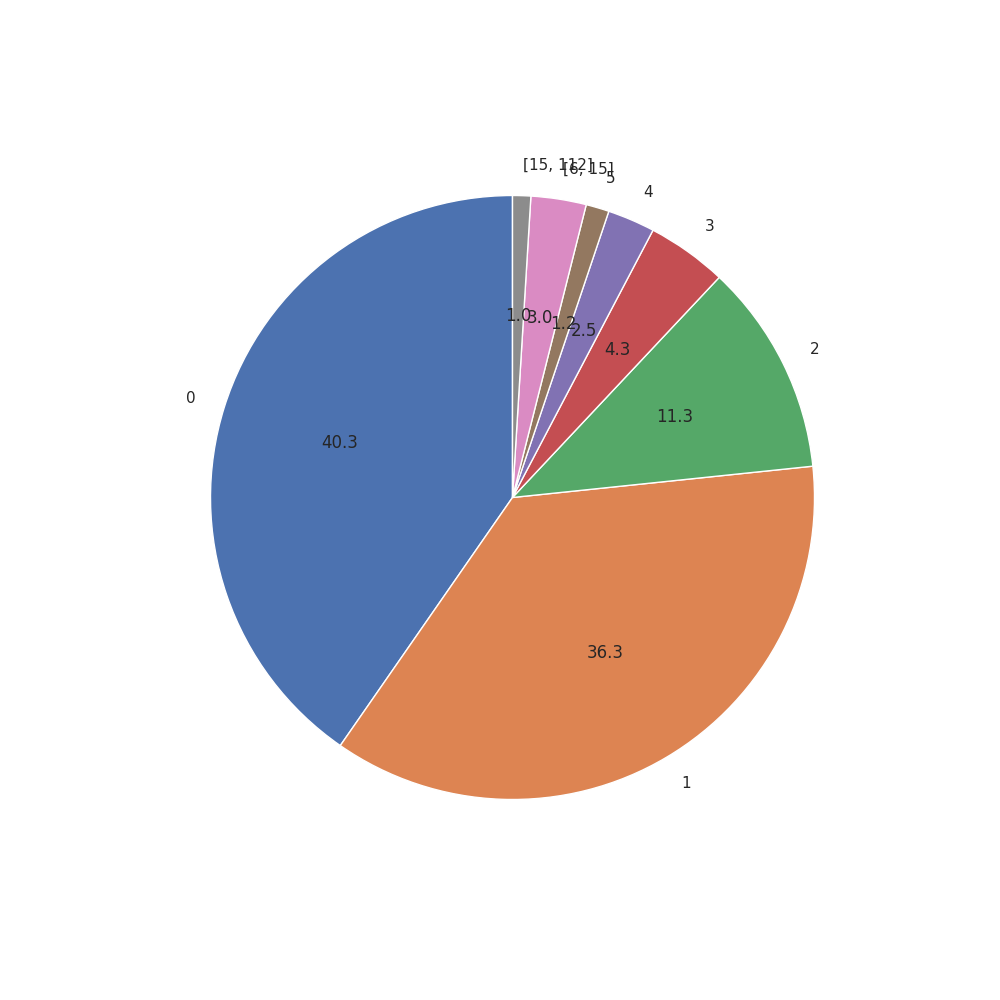
\includegraphics[width=7.3cm, trim={1.1cm 0cm 0.6cm 2cm}, clip]{images/retinafocus_iou_75_lower}} 
        \subfigure[]{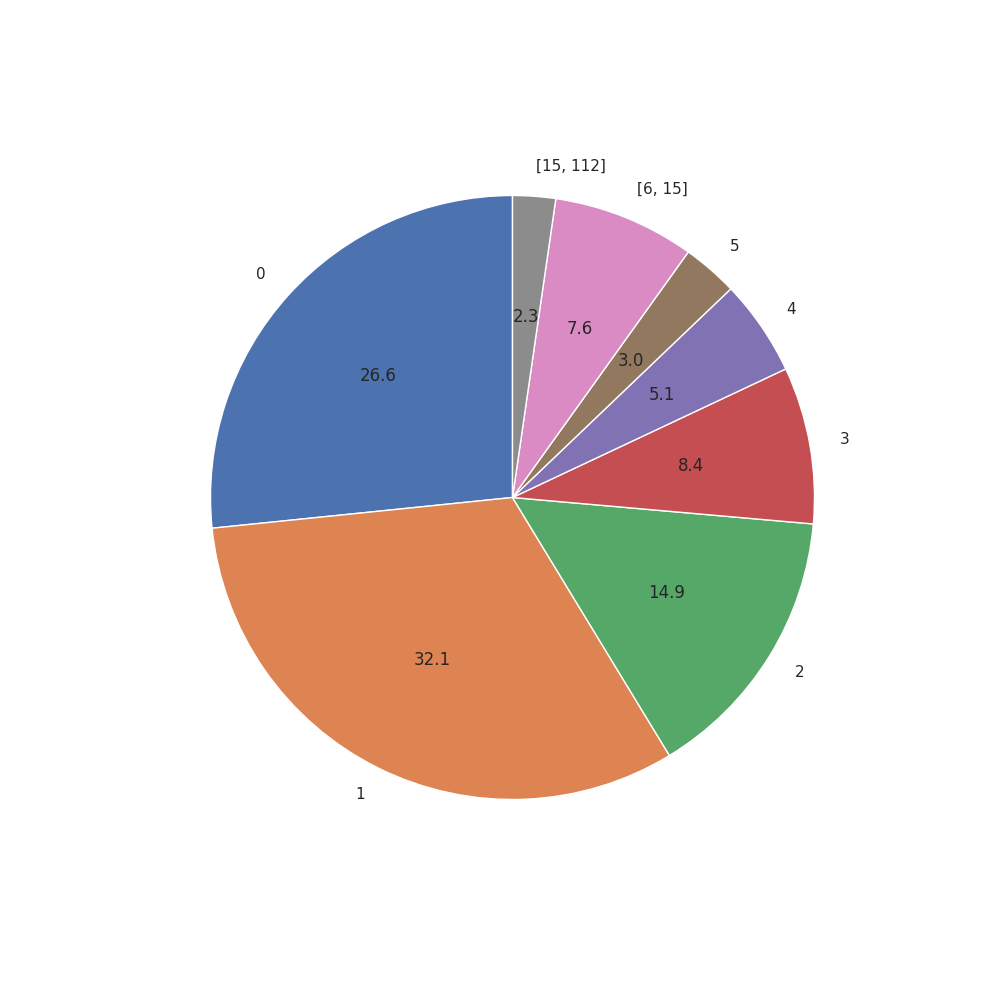
\includegraphics[width=7.3cm, trim={1.1cm 0cm 0.6cm 2cm}, clip]{images/retinafocus_iou_90_lower}} 
        \caption{Tỷ lệ các kích thước của hộp giới hạn\index{hộp giới hạn} mà RetinaFace không dự đoán ra tương ứng với IoU\index{IoU} 0.5 (a), IoU\index{IoU} 0.75 (b), IoU\index{IoU} 0.9 (c)}
        \label{fig:retinafocus_iou_lower}
    \end{figure}

    \noindent
    Từ những phân tích trên, chúng tôi lựa chọn lần lượt các tham số $a = 5, b = 60, c = 150$ tương ứng với groundtruth\index{groundtruth} hộp giới hạn\index{hộp giới hạn} có kích thước từ $5 \times 5$ đến $60 \times 60$ là các hộp giới hạn\index{hộp giới hạn} cần được focus, các groundtruth\index{groundtruth} hộp giới hạn\index{hộp giới hạn} có kích thước dưới $5 \times 5$ hoặc từ $60 \times 60$ đến $150 \times 150$ là các hộp giới hạn\index{hộp giới hạn} không cần quan tâm và các groundtruth\index{groundtruth} hộp giới hạn\index{hộp giới hạn} có kích thước trên $150 \times 150$ là các hộp giới hạn\index{hộp giới hạn} được coi như là background\index{background}. \\

    \noindent
    \textbf{\textit{Thuật toán sinh Focus Chips}} \\
    Dựa trên AutoFocus \cite{najibi2019autofocus}, sau khi mô hình đã được huấn luyện và dự đoán ra được điểm ảnh\index{điểm ảnh} cần được focus, mô hình cần một thuật toán để crop ra được khu vực cần focus trên ảnh làm đầu vào cho cả hai nhánh xác định đối tượng\index{nhánh xác định đối tượng} và nhánh tập trung đối tượng\index{nhánh tập trung đối tượng} ở nhữnglượt tiếp theo.
    Và đó là vai trò của thuật toán sinh Focus Chips.

    \begin{figure}[H]
        \centering
        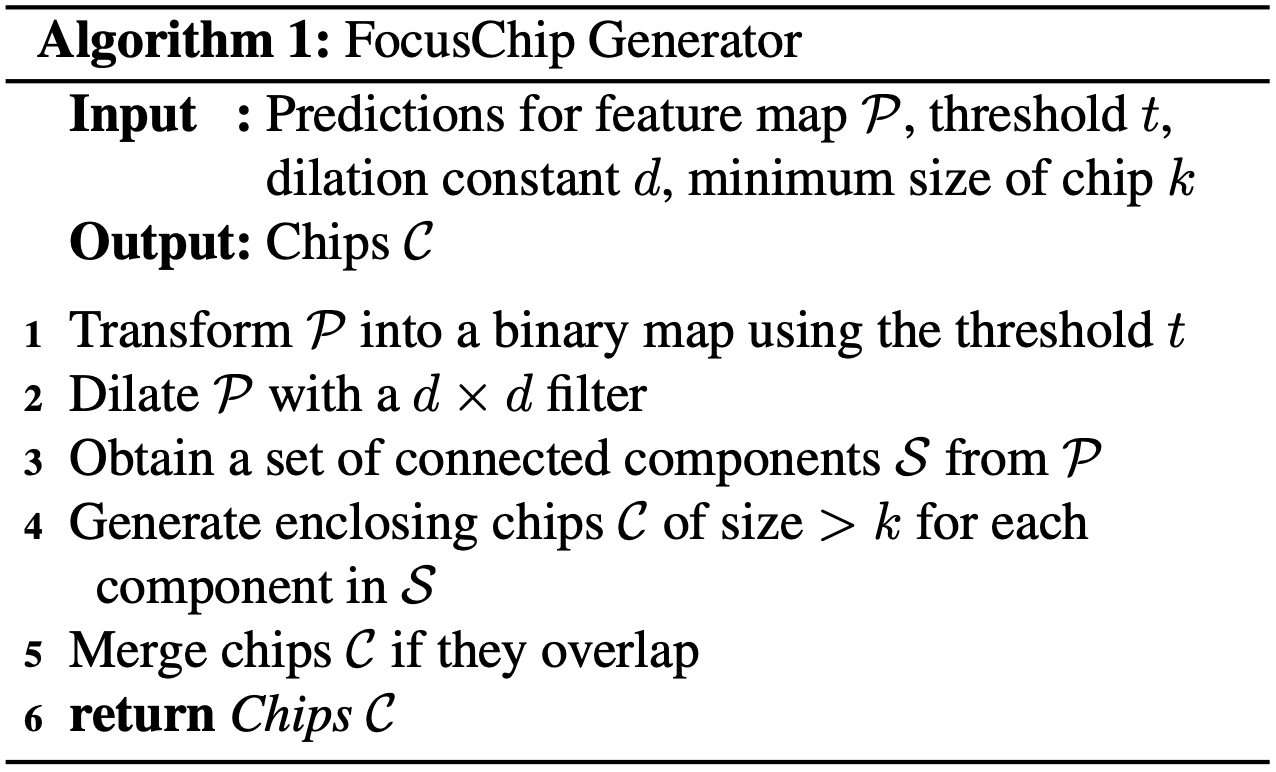
\includegraphics[width=10cm] {images/autofocus_focus_chip_gen}
        \caption{Chi tiết thuật toán sinh Focus Chips (Nguồn: \cite{najibi2019autofocus})}
        \label{fig:autofocus_focus_chip_gen}
    \end{figure}

    \noindent
    Trong quá trình dự đoán, sau khi mô hình đã dự đoán được các điểm ảnh\index{điểm ảnh} cần được focus (ký hiệu là $\mathcal{P}$) trên Focus Pixel  mask, ta biến đổi mask này trở về dạng binary mask bằng threshold $t$.
    Tham số $t$ được sử dụng để cân đối giữa tốc độ và độ chính xác của mô hình (cụ thể với tham số $t$ lớn, số lượng các điểm ảnh\index{điểm ảnh} cần được focus sẽ giảm đi và tốc độ của mô hình AutoFocus sẽ tăng và ngược lại). \\
    Từ binary mask đã được sinh ra ở trên, thuật toán sinh Focus Chips sẽ đưa qua một filter có kích thước $d \times d$ nhằm giãn nở các điểm ảnh\index{điểm ảnh} thêm một chút để thu được các thành phần liên thông $\mathcal{S}$, từ đó có nhiều thông tin hơn khi crop ảnh đầu vào với các focus điểm ảnh\index{điểm ảnh} này. \\
    Cuối cùng, ta crop ra các chip $\mathcal{C}$ với kích thước tối thiểu là $k \times k$ và bao trọn các thành phần liên thông $\mathcal{S}$ trên.
    Các chip trong $\mathcal{C}$ nếu có overlap với nhau sẽ được gộp lại chung thành một chip. \\
    Việc sinh ra các chip $\mathcal{C}$ giúp mô hình AutoFocus có thể sử dụng ý tưởng Image Pyramids nhưng tiết kiệm chi phí tính toán nhờ loại bỏ các khu vực khả năng cao không chứa đối tượng. \\

    \noindent
    \textbf{\textit{Thuật toán Focus Stacking}} \\
    Một vấn đề cần phải giải quyết khi thực hiện dự đoán với ý tưởng Image Pyramids trong bài toán nhận diện đối tượng\index{nhận diện đối tượng} là việc tổng hợp lại các hộp giới hạn\index{hộp giới hạn}.

    \begin{figure}[H]
        \centering
        \includegraphics[width=15cm] {images/autofocus_focus_stack}
        \caption{Ví dụ về cơ chế hoạt động của thuật toán Focus Stacking (Nguồn: \cite{najibi2019autofocus})}
        \label{fig:autofocus_focus_stack}
    \end{figure}

    \noindent
    Với ý tưởng từ AutoFocus \cite{najibi2019autofocus}, vấn đề này còn phức tạp hơn với trường hợp một đối tượng có kích thước lớn được dự đoán ở kích thước này, nhưng đến kích thước tiếp theo, đối tượng đó bị crop trong quá trình crop chip và trở thành một đối tượng có kích thước nhỏ hơn.
    Nhằm hạn chế bớt vấn đề này, nhóm tác giả chỉ ra rằng \textit{bước 2} trong thuật toán sinh Focus Chips \ref{fig:autofocus_focus_chip_gen} là cực kỳ quan trọng.

    \noindent
    Tuy nhiên, nhóm tác giả cũng đề ra một số luật nhằm loại bỏ các dự đoán lỗi của các đối tượng được định vị trên một focus chip: \\
    - Nếu một đối tượng nằm trên một biên của chip nhưng không phải biên của ảnh đầu vào (nghĩa là đối tượng này đã bị crop sau khi qua thuật toán sinh Focus Chip), thì dự đoán sẽ bị loại bỏ. \\
    - Nếu một đối tượng nằm trên một biên của chip và đó là biên của ảnh đầu vào, nhóm tác giả sẽ tiếp tục kiểm tra biên còn lại của đối tượng, nếu đó là biên của chip, dự đoán sẽ bị loại, còn nếu đó không phải là biên của chip, dự đoán sẽ được giữ lại. \\
    - Nếu một đối tượng nằm trên hai biên của chip và đó đều là hai biên của ảnh đầu vào, nhóm tác giả sẽ giữ lại những dự đoán này. \\
    Sau khi loại bỏ bớt các dự đoán bằng thuật toán Focus Stacking, mô hình AutoFocus đưa ra tổng hợp dự đoán từ các kích thước ảnh khác nhau và là các dự đoán cuối cùng của ảnh đầu vào.
}
    \autofocus


}
    \retinafocusarchitecture

}

    \proposedmodel

    \newpage
    \def\datasetsandexperiments{
    \section{Dữ liệu và thực nghiệm}
    Các bộ dữ liệu nổi tiếng được sử dụng nhiều trong các bài toán học sâu như ImageNet \cite{russakovsky2015imagenet}, MS-COCO \cite{lin2014microsoft} hay PASCAL-VOC \cite{everingham2010pascal} đều có đặc điểm chung là kích thước ảnh nhỏ, khoảng dưới 1500 pixels.
    % Những bộ dữ liệu mới gần đây như PANDA \cite{},  đã chứa nhiều ảnh có kích thước lớn, tuy nhiên, ....

    \noindent
    Đối với bài toán nhận diện khuôn mặt, một số bộ dữ liệu như FDDB \cite{jain2010fddb}, ALW \cite{zhu2012face}, AFLW \cite{koestinger2011annotated}, 300 Faces in-the-Wild Challenge \cite{sagonas2013300}, PASCAL Face \cite{yan2014face} và WIDER FACE \cite{yang2016wider} thường được sử dụng để đánh giá chất lượng của mô hình.
    Tuy nhiên, các bộ dữ liệu này vẫn gồm các ảnh có kích thước nhỏ, khoảng dưới 1500 pixels, nên việc đánh giá đúng về độ chính xác và tốc độ của mô hình giải quyết bài toán nhận diện khuôn mặt trên ảnh chất lượng cao gặp nhiều khó khăn.

    \subsection{Bộ dữ liệu WIDER FACE}
    \def\widerface{
    Bộ dữ liệu WIDER FACE \cite{yang2016wider} là một bộ dữ liệu nổi tiếng được sử dụng rộng rãi dành cho bài toán nhận diện khuôn mặt.
    Bộ dữ liệu WIDER FACE được nhóm tác giả nhấn mạnh về tính thực tiễn do có chứa ảnh đa dạng và gần với các khung cảnh trong thực tế.
    Bộ dữ liệu chứa rất nhiều ảnh với các khuôn mặt đa dạng trong tỷ lệ kích thước, kiểu dáng, biểu cảm, che chắn, góc quay và ánh sáng.
    Hơn nữa số lượng ảnh của bộ WIDER FACE cũng lớn hơn rất nhiều so với các bộ dữ liệu về mặt ở thời điểm đó.
    
    \begin{figure}[H]
        \centering
        \includegraphics[width=15cm] {images/widerface_compare_1}
        \caption{So sánh về số lượng và độ đa dạng của bộ dữ liệu WIDER FACE với một số bộ dữ liệu khác (Nguồn: \cite{yang2016wider})}
        \label{fig:widerface_compare_1}
    \end{figure}

    \subsubsection*{Các thông số của bộ dữ liệu WIDER FACE}
    Bộ dữ liệu WIDER FACE bao gồm 32,203 ảnh với 393,703 hộp giới hạn\index{hộp giới hạn} của khuôn mặt với sự đa dạng về kích thước, góc quay, che chắn.
    Bộ dữ liệu WIDER FACE được chụp từ 61 khung cảnh khác nhau, trong đó, với mỗi khung cảnh, nhóm tác giả chia thành ba bộ train/val/test theo tỷ lệ 40\%/10\%/50\%.

    \noindent
    Nhóm tác giả của bộ dữ liệu WIDER FACE sử dụng mô hình EdgeBox \cite{zitnick2014edge} để chia bộ dữ liệu thành ba mức độ khó (bộ Dễ, bộ Trung bình và bộ Khó).
    Trong đó, mô hình EdgeBox đạt mức recall lần lượt tương ứng với bộ Dễ, bộ Trung bình và bộ Khó là 92\%, 76\% và 34\%.
    Mô hình EdgeBox đạt kết quả kém hơn rất nhiều trên bộ WIDER FACE so sánh với kết quả trên các bộ dữ liệu khác.

    \begin{figure}[H]
        \centering
        \includegraphics[width=10cm] {images/widerface_compare_2}
        \caption{So sánh độ khó của bộ dữ liệu WIDER FACE với các bộ dữ liệu khác (Nguồn: \cite{yang2016wider})}
        \label{fig:widerface_compare_2}
    \end{figure}

    \begin{figure}[H]
        \centering
        \includegraphics[width=15cm] {images/widerface_examples}
        \caption{Một số ví dụ trong bộ dữ liệu WIDER FACE (Nguồn: \cite{yang2016wider})}
        \label{fig:widerface_examples}
    \end{figure}

    \subsubsection*{Bộ dữ liệu WIDER FACE với landmarks}
    Nhóm tác giả của mô hình RetinaFace \cite{deng2020retinaface} đã bổ sung thêm vào bộ dữ liệu WIDER FACE thông tin về landmarks của các khuôn mặt bao gồm 5 điểm: tâm của mắt trái, tâm của mắt phải, đỉnh của mũi, điểm mép miệng trái và điểm mép miệng phải.

    \begin{figure}[H]
        \centering
        \includegraphics[width=10cm] {images/widerface_five_levels_lm_1}
        \caption{Ví dụ về mức độ khó của khuôn mặt trong việc gán landmarks (Nguồn: \cite{deng2020retinaface})}
        \label{fig:widerface_five_levels_lm_1}
    \end{figure}

    \noindent
    Dựa vào chất lượng của ảnh, nhóm tác giả đã chia bộ dữ liệu thành 5 mức độ khó: \\
    - Độ khó 1 (dễ nhất): Dễ dàng gán nhãn được 68 điểm landmarks của mặt. \\
    - Độ khó 2: Có thể gán nhãn được 68 điểm landmarks của mặt. \\
    - Độ khó 3: Dễ dàng gán nhãn được 5 điểm landmarks của mặt. \\
    - Độ khó 4: Có thể gán nhãn được 5 điểm landmarks của mặt. \\
    - Độ khó 5 (khó nhất): Chỉ có thể phân biệt được với background\index{background} của ảnh. Với các hộp giới hạn\index{hộp giới hạn} ở mức độ khó này, nhóm tác giả không gán 5 điểm landmarks. \\
    Dựa vào các mức độ khó nói trên, nhóm tác giả của RetinaFace đã gán landmarks cho các khuôn mặt trong hai tập dữ liệu huấn luyện và val, tương ứng 84.6k mặt cho tập huấn luyện và 18.5k mặt cho bộ val.

    \begin{figure}[H]
        \centering
        \includegraphics[width=11cm] {images/widerface_five_levels_lm_2}
        \caption{Các thông số của độ khó của khuôn mặt trong việc gán landmarks (Nguồn: \cite{deng2020retinaface})}
        \label{fig:widerface_five_levels_lm_2}
    \end{figure}

    \subsubsection*{Vấn đề tồn đọng của bộ dữ liệu WIDER FACE}
    Ở thời điểm ra mắt, bộ dữ liệu WIDER FACE thật sự là một bước tiến về dữ liệu cho bài toán nhận diện khuôn mặt bởi số lượng và sự đa dạng.
    Tuy nhiên, cho đến nay, kích thước như ảnh trong bộ WIDER FACE khoảng 1000 - 1500 điểm ảnh\index{điểm ảnh} không còn là kích thước lớn nữa.
    Điều này là rào cản cho giới nghiên cứu khi phát triển các mô hình giải quyết bài toán nhận diện khuôn mặt trong ảnh chất lượng cao.
}
    \widerface

    \subsection{Bộ dữ liệu WIDER FACE 4K}
    \def\widerfacefourk{
    Kế thừa những điểm mạnh về sự đa dạng của khuôn mặt trong bộ dữ liệu WIDER FACE \cite{yang2016wider}, tôi đề xuất một phương pháp xây dựng bộ dữ liệu WIDER FACE kích thước lớn gồm có nhiều ảnh có độ phân giải cao, giúp đánh giá khách quan độ chính xác và tốc độ của các mô hình giải bài toán nhận diện khuôn mặt với ảnh chất lượng cao.

    \begin{figure}[H]
        \centering
        \subfigure[]{\includegraphics[width=7.3cm]{images/widerface_highres_1}}
        \subfigure[]{\includegraphics[width=7.3cm]{images/widerface_highres_2}}
        \subfigure[]{\includegraphics[width=9.4cm]{images/widerface_highres_3}}
        \caption{Một ví dụ ảnh trong bộ dữ liệu WIDER FACE \cite{yang2016wider} (a) so sánh với bộ dữ liệu WIDER FACE kích thước lớn dạng lưới $2 X 2$ (b) và $3 X 3$ (c)}
        \label{fig:widerface_4k_example}
    \end{figure}

    \subsubsection*{Ý tưởng xây dựng bộ dữ liệu WIDER FACE kích thước lớn}
    Nhằm tận dụng hết những điểm mạnh như tỷ lệ kích thước, kiểu dáng, biểu cảm, che chắn, góc quay và ánh sáng của bộ dữ liệu WIDER FACE, tôi không tác động gì đến dữ liệu ảnh của bộ dữ liệu WIDER FACE mà chỉ nối chúng lại với nhau theo dạng lưới nhằm tạo ra bộ dữ liệu ảnh có kích thước lớn hơn.
    Với số lượng cũng như độ đa dạng của khuôn mặt được giữ nguyên của bộ dữ liệu WIDER FACE, nhưng với kích thước ảnh lớn hơn, bộ dữ liệu WIDER FACE kích thước lớn sẽ đánh giá tốt khả năng của các mô hình nhận diện khuôn mặt, không chỉ ở độ chính xác, mà còn ở thời gian chạy cũng như khối lượng bộ nhớ cần dùng.

    \noindent
    Trong khuôn khổ của luận văn, tôi chỉ xây dựng các bộ dữ liệu WIDER FACE kích thước lớn với dạng lưới có kích thước $2 X 2$, và $3 X 3$, tuy nhiên, ý tưởng xây dựng bộ dữ liệu WIDER FACE kích thước lớn này hoàn toàn có thể áp dụng với các kích thước lưới lớn hơn $n X n$ nhằm tạo ra bộ dữ liệu ảnh có kích thước lớn hơn nữa.

    \begin{figure}[H]
        \centering
        \subfigure[]{\includegraphics[width=7.3cm, trim={0.5cm 0.5cm 3cm 2cm}, clip]{images/widerface_nk_img_size_1K}}
        \subfigure[]{\includegraphics[width=7.3cm, trim={0.5cm 0.5cm 3cm 2cm}, clip]{images/widerface_nk_img_size_2K}}
        \subfigure[]{\includegraphics[width=7.3cm, trim={0.5cm 0.5cm 3cm 2cm}, clip]{images/widerface_nk_img_size_3K}}
        \caption{Phân phối về kích thước ảnh trong bộ dữ liệu WIDER FACE \cite{yang2016wider} (a) so sánh với bộ dữ liệu WIDER FACE kích thước lớn dạng lưới $2 X 2$ (b) và $3 X 3$ (c)}
        \label{fig:widerface_4k_img_size}
    \end{figure}

    \subsubsection*{Các thông số của bộ dữ liệu WIDER FACE kích thước lớn}
    Bộ dữ liệu WIDER FACE kích thước lớn, đúng với mục đích ra đời, đã làm tăng kích thước dữ liệu ảnh đáng kể.
    So sánh với bộ dữ liệu WIDER FACE với kích thước ảnh trung bình nằm trong khoảng từ 750 đến 1250 điểm ảnh mỗi chiều, bộ dữ liệu WIDER FACE kích thước lớn đã tăng kích thước ảnh trung bình từ 1500 đến 2500 điểm ảnh mỗi chiều đối với dạng lưới $2 X 2$ và 2200 đến 4000 điểm ảnh mỗi chiều đối với dạng lưới $3 X 3$.

    \noindent
    Hơn nữa, kích thước ảnh tối đa trên bộ dữ liệu WIDER FACE kích thước lớn cũng được cải thiện, so sánh với kích thước 2250 điểm ảnh của bộ dữ liệu WIDER FACE, bộ dữ liệu WIDER FACE kích thước lớn có kích thước ảnh tối đa là 4500 điểm ảnh với dạng lưới $2 X 2$ và 7000 điểm ảnh với dạng lưới $3 X 3$.

    \begin{figure}[H]
        \centering
        \subfigure[]{\includegraphics[width=7.3cm, trim={0.5cm 0.5cm 3cm 3cm}, clip]{images/widerface_nk_scale_1K}}
        \subfigure[]{\includegraphics[width=7.3cm, trim={0.5cm 0.5cm 3cm 3cm}, clip]{images/widerface_nk_scale_2K}}
        \subfigure[]{\includegraphics[width=7.3cm, trim={0.2cm 0.5cm 3cm 3cm}, clip]{images/widerface_nk_scale_3K}}
        \caption{Phân phối về tỷ lệ giữa kích thước của hộp giới hạn và kích thước ảnh trong bộ dữ liệu WIDER FACE \cite{yang2016wider} (a) so sánh với bộ dữ liệu WIDER FACE kích thước lớn dạng lưới $2 X 2$ (b) và $3 X 3$ (c)}
        \label{fig:widerface_4k_scale}
    \end{figure}

    \noindent
    Với việc kích thước ảnh được tăng lên đáng kể, việc nhận diện các khuôn mặt trong ảnh trở nên khó khăn hơn, đặc biệt là với các khuôn mặt có kích thước nhỏ.
    Trong bộ dữ liệu WIDER FACE kích thước lớn, số lượng các mặt có kích thước nhỏ so sánh tỷ lệ với kích thước ảnh trong bộ dữ liệu lớn hơn.
    Cụ thể, đối với bộ dữ liệu WIDER FACE, trung bình kích thước hộp giới hạn của khuôn mặt bằng khoảng 2\% kích thước của ảnh.

    \noindent
    Đối với bộ dữ liệu WIDER FACE kích thước lớn, trung bình kích thước hộp giới hạn của khuôn mặt bằng khoảng 1\% kích thước của ảnh đối với dạng lưới $2 X 2$ và 0.6\% kích thước của ảnh đối với dạng lưới $3 X 3$.

    \noindent
    Với những thông số trên, bộ dữ liệu WIDER FACE kích thước lớn được kỳ vọng giúp đánh giá khách quan độ chính xác và tốc độ của các mô hình giải bài toán nhận diện khuôn mặt với ảnh chất lượng cao.
}
    \widerfacefourk

    \subsection{Các thí nghiệm và kết quả của mô hình RetinaFocus}
    \def\retinafocusresults{
    Một đặc điểm của mô hình RetinaFocus là có nhiều cấu hình có thể cài đặt để triển khai mô hình như cấu hình lựa chọn feature maps \index{feature maps} của FPN cho Nhánh Focus \index{nhánh Focus}, cấu hình scale ảnh trong quá trình predict \dots
    Vì vậy, ta cần so sánh và lựa chọn cấu hình tối ưu nhất, cân đối giữa thời gian thực hiện quá trình predict và độ chính xác của mô hình.
    Để so sánh một cách toàn diện nhất, ta sẽ sử dụng cả hai bộ dữ liệu WIDER FACE thông thường và bộ dữ liệu WIDER FACE 4K đã được giới thiệu ở \textbf{\textit{phần 5.2}}.

    \noindent
    \textbf{\textit{Thí nghiệm so sánh cấu hình sử dụng feature maps \index{feature maps} khác nhau của FPN làm đầu vào cho Nhánh Focus}} \index{nhánh Focus} \\
    Trong thí nghiệm này, với mỗi cấu hình, chúng tôi sử dụng các feature maps \index{feature maps} khác nhau của FPN làm đầu vào cho Nhánh Focus \index{nhánh Focus}.
    Trong đó, lần lượt các cấu hình sử dụng feature maps \index{feature maps} ${C}_{3}, {C}_{4}, {C}_{5}, {P}_{3}, {P}_{4}, {P}_{5}$ được ký hiệu là \textit{C3}, \textit{C4}, \textit{C5}, \textit{P3}, \textit{P4}, \textit{P5} trong các biểu đồ.
    Trong các cấu hình trên, các cặp feature maps \index{feature maps} ${C}_{3}$ và ${P}_{3}$, ${C}_{4}$ và ${P}_{4}$, ${C}_{5}$ và ${P}_{5}$ là các cặp feature maps \index{feature maps} có cùng kích thước.
    Tuy nhiên, mỗi feature maps \index{feature maps} khác nhau trong cặp chứa thông tin khác nhau về khuôn mặt dẫn đến số lượng và kích thước của các vùng mà Nhánh Focus \index{nhánh Focus} xác định cần phải zoom vào cũng khác nhau.
    Từ đó dẫn đến thời gian thực hiện toàn bộ quá trình predict trên cả bộ dữ liệu là khác nhau.
    Trong thí nghiệm này, các cấu hình sử dụng chung một cấu hình scale ảnh trong quá trình predict là ....

    \begin{figure}[H]
        \centering
        \subfigure[]{\includegraphics[width=0.32\textwidth, trim={2.3cm 2.3cm 2.3cm 2.3cm}, clip]{images/retinafocus_widerface_val_easy_fpn}} 
        \subfigure[]{\includegraphics[width=0.32\textwidth, trim={2.3cm 2.3cm 2.3cm 2.3cm}, clip]{images/retinafocus_widerface_val_medium_fpn}} 
        \subfigure[]{\includegraphics[width=0.32\textwidth, trim={2.3cm 2.3cm 2.3cm 2.3cm}, clip]{images/retinafocus_widerface_val_hard_fpn}} 
        \caption{Kết quả so sánh các cấu hình sử dụng các feature maps \index{feature maps} của FPN làm đầu vào cho Nhánh Focus \index{nhánh Focus} trên ba bộ dữ liệu WIDER FACE val easy (a), medium (b) và hard (c)}
        \label{fig:retinafocus_widerface_val_fpn}
    \end{figure}

    \noindent
    Đối với bộ WIDER FACE thông thường, hai cấu hình đạt độ chính xác cao nhất là cấu hình sử dụng feature maps \index{feature maps} ${P}_{5}$ và cấu hình sử dụng feature maps \index{feature maps} ${C}_{5}$ cho Nhánh Focus \index{nhánh Focus} với thời gian thực hiện toàn bộ quá trình predict trên cả bộ dữ liệu lần lượt là ... và ....
    Trong khi cấu hình sử dụng feature maps \index{feature maps} ${P}_{5}$ cho kết quả tốt hơn trên bộ WIDER FACE val easy và medium thì cấu hình sử dụng feature maps \index{feature maps} ${C}_{5}$ cho kết quả tốt hơn trên bộ WIDER FACE val hard.
    Các cấu hình khác như ${P}_{4}$, ${P}_{3}$ và ${C}_{4}$ có thời gian thực hiện toàn bộ quá trình predict nhanh hơn nhưng độ chính xác không tốt.
    Đặc biệt là cấu hình ${C}_{3}$ vừa có thời gian thực hiện toàn bộ quá trình predict chậm vừa đạt độ chính xác thấp.

    \begin{figure}[H]
        \centering
        \subfigure[]{\includegraphics[width=0.32\textwidth, trim={2.3cm 2.3cm 2.3cm 2.3cm}, clip]{images/retinafocus_widerface_4k_val_easy_fpn}} 
        \subfigure[]{\includegraphics[width=0.32\textwidth, trim={2.3cm 2.3cm 2.3cm 2.3cm}, clip]{images/retinafocus_widerface_4k_val_medium_fpn}} 
        \subfigure[]{\includegraphics[width=0.32\textwidth, trim={2.3cm 2.3cm 2.3cm 2.3cm}, clip]{images/retinafocus_widerface_4k_val_hard_fpn}} 
        \caption{Kết quả so sánh các cấu hình sử dụng các feature maps \index{feature maps} của FPN làm đầu vào cho Nhánh Focus \index{nhánh Focus} trên ba bộ dữ liệu WIDER FACE 4K val easy (a), medium (b) và hard (c)}
        \label{fig:retinafocus_widerface_4k_val_fpn}
    \end{figure}

    \noindent
    Đối với bộ WIDER FACE 4K, hai cấu hình đạt độ chính xác cao nhất vẫn là cấu hình sử dụng feature maps \index{feature maps} ${P}_{5}$ và cấu hình sử dụng feature maps \index{feature maps} ${C}_{5}$ với thời gian thực hiện toàn bộ quá trình predict trên cả bộ dữ liệu lần lượt là ... và ....
    Đối với bộ dữ liệu này, cấu hình sử dụng feature maps \index{feature maps} ${P}_{5}$ cho kết quả tốt hơn so với cấu hình sử dụng feature maps \index{feature maps} ${C}_{5}$ trên cả ba bộ WIDER FACE 4K val easy, medium và hard.

    \noindent
    Kết luận đối với thí nghiệm này là cấu hình sử dụng feature maps \index{feature maps} ${P}_{5}$ đạt kết quả tốt nhất về độ chính xác trong khi vẫn duy trì được thời gian thực hiện toàn bộ quá trình predict tương đối nhanh.

    \noindent
    \textbf{\textit{Thí nghiệm so sánh cấu hình scale ảnh tốt nhất trong quá trình predict}} \\

    \noindent
    \textbf{\textit{Thí nghiệm so sánh cấu hình tốt nhất của RetinaFocus với các cấu hình của RetinaFace}} \\
    Các cấu hình của mô hình RetinaFace sử dụng trong thí nghiệm này bao gồm: \\
    - Cấu hình sử dụng chiến lược Image Pyramids kết hợp với việc lật ảnh đầu vào trong quá trình predict, ký hiệu là \dots \\
    - Cấu hình chỉ sử dụng chiến lược Image Pyramids, ký hiệu là \dots \\
    - Cấu hình không sử dụng chiến lược Image Pyramids mà chỉ sử dụng một scale ảnh duy nhất là [1200, 1600], ký hiệu là \dots \\
    - Cấu hình không sử dụng chiến lược Image Pyramids mà chỉ sử dụng một scale ảnh duy nhất là [1504, 2000], ký hiệu là \dots \\
    - Cấu hình không sử dụng chiến lược Image Pyramids mà chỉ sử dụng một scale ảnh duy nhất là [1600, 2150], ký hiệu là \dots \\

    \begin{figure}[H]
        \centering
        \subfigure[]{\includegraphics[width=0.32\textwidth, trim={2.3cm 2.3cm 2.3cm 2.3cm}, clip]{images/retinafocus_widerface_val_easy_rtnf}} 
        \subfigure[]{\includegraphics[width=0.32\textwidth, trim={2.3cm 2.3cm 2.3cm 2.3cm}, clip]{images/retinafocus_widerface_val_medium_rtnf}} 
        \subfigure[]{\includegraphics[width=0.32\textwidth, trim={2.3cm 2.3cm 2.3cm 2.3cm}, clip]{images/retinafocus_widerface_val_hard_rtnf}} 
        \caption{Kết quả so sánh cấu hình tốt nhất của RetinaFocus với các cấu hình của RetinaFace trên ba bộ dữ liệu WIDER FACE val easy (a), medium (b) và hard (c)}
        \label{fig:retinafocus_widerface_val_rtnf}
    \end{figure}

    \begin{figure}[H]
        \centering
        \subfigure[]{\includegraphics[width=0.32\textwidth, trim={2.3cm 2.3cm 2.3cm 2.3cm}, clip]{images/retinafocus_widerface_4k_val_easy_rtnf}} 
        \subfigure[]{\includegraphics[width=0.32\textwidth, trim={2.3cm 2.3cm 2.3cm 2.3cm}, clip]{images/retinafocus_widerface_4k_val_medium_rtnf}} 
        \subfigure[]{\includegraphics[width=0.32\textwidth, trim={2.3cm 2.3cm 2.3cm 2.3cm}, clip]{images/retinafocus_widerface_4k_val_hard_rtnf}} 
        \caption{Kết quả so sánh cấu hình tốt nhất của RetinaFocus với các cấu hình của RetinaFace trên ba bộ dữ liệu WIDER FACE 4K val easy (a), medium (b) và hard (c)}
        \label{fig:retinafocus_widerface_val_rtnf}
    \end{figure}

}
    \retinafocusresults

}

    \datasetsandexperiments

    % % KET THUC PHAN NOI DUNG CHINH

    % BAT DAU CAC TRANG CHUC NANG KHAC
    % Xoa header - footer
    
    \newpage
    \pagestyle{plain}
    \def \tongket{
    \section*{Kết luận và phương hướng phát triển}
    \addcontentsline{toc}{section}{Kết luận và phương hướng phát triển}
    Với sự phát triển của khoa học công nghệ, kích thước của ảnh trong thực tế cuộc sống ngày càng tăng và điều đó đòi hỏi các mô hình học sâu xử lý với độ chính xác cao và tốc độ nhanh.
    Rào cản này đã phần nào đó được vượt qua thông qua các nghiên cứu trong những năm trở lại đây, giúp việc xử lý ảnh chất lượng cao trở nên dễ dàng và chính xác hơn. \\
    Hai đóng góp chính của luận văn bao gồm: \\
    - Mô hình RetinaFocus giúp cải thiện độ chính xác và tốc độ của các mô hình học sâu giải quyết bài toán nhận diện khuôn mặt với trong ảnh chất lượng cao rất nhiều.
    So sánh với mô hình nguyên bản, mô hình RetinaFocus đã tăng tốc ... trong khi duy trì được độ chính xác tương đương trên bộ dữ liệu WIDER FACE. \\
    - Bộ dữ liệu WIDER FACE kích thước lớn đã giúp đánh giá một cách chính xác và khách quan độ chính xác và tốc độ của mô hình RetinaFocus trong việc xử lý ảnh chất lượng cao, so sánh với kết quả của mô hình nguyên bản. \\
    Từ đó, mô hình RetinaFocus sẽ là nền tảng cho các nghiên cứu khác giải quyết bài toán nhận diện khuôn mặt cũng như là nhận diện đối tượng\index{nhận diện đối tượng} trong ảnh chất lượng cao trong tương lai.
}
    \tongket

    \newpage
    \printindex

    \newpage
    \addcontentsline{toc}{section}{Tài liệu tham khảo}
    \renewcommand\refname{Tài liệu tham khảo}
    \bibliography{references.bib}
    \bibliographystyle{unsrt}
    % KET THUC CAC TRANG CHUC NANG KHAC

\end{document}